\documentclass[aspectratio=169,t]{beamer}
\usepackage[utf8]{inputenc}
\usepackage[T1]{fontenc}
\usepackage[english]{babel}
\usepackage{hyperref}
\usepackage{tikz}

\usepackage{graphicx}
\usepackage{epstopdf}
\usepackage{multirow}

\usepackage{psfrag}
\usepackage{pgfplots}
\usepackage{framed}
\usepackage{xcolor}
\usepackage{booktabs}
\usepackage{caption}
\usepackage{epstopdf}
\usepackage{amsmath}
\usepackage{tabularx}
\usepackage[]{bookmark}
%\usepackage[3D]{movie15}
%\usepackage{media9}
\usepackage[binary-units,abbreviations]{siunitx}
\usepackage[textfont=normalsize, labelfont=normalsize, justification=centering]{subcaption}
\usepackage{marvosym}
\usepackage{calc}
\usepackage{color, colortbl}
\usepackage[]{svg} 
\usepackage[]{trfsigns} 
\usepackage[nomessages]{fp}
\usepackage[]{csquotes}\MakeOuterQuote{"}
\usepackage{tabto}
\selectcolormodel{rgb}

\makeatletter
\def\beamer@calltheme#1#2#3{\def\beamer@themelist{#2}
	\@for\beamer@themename:=\beamer@themelist\do
	{\usepackage[{#1}]{\beamer@themelocation/#3\beamer@themename}}}
\def\usefolder#1{\def\beamer@themelocation{#1}}
\def\beamer@themelocation{}
\usefolder{theme}

\usetikzlibrary{matrix,
	decorations.pathreplacing,
	calc,
	positioning,
	external,
	3d,
	shapes,
	arrows,
	pgfplots.statistics}
\pgfplotsset{compat=1.16}
\tikzstyle{faunode}=[rounded corners, draw=faublue, fill=faublue!10,  align=center, inner sep=0.3cm, line width=0.4mm]
\tikzstyle{fauellipseFixedWidth}=[ellipse, draw=faublue, fill=faublue!10,  align=center, inner sep=0.3cm, line width=0.4mm, minimum width=3cm]
\tikzstyle{fauellipse}=[ellipse, draw=faublue, fill=faublue!10,  align=center, inner sep=0.3cm, line width=0.4mm]
\tikzstyle{fauarrow}=[draw=faublue,->, line width=0.4mm]
\tikzstyle{fauline}=[draw=faublue, line width=0.4mm]


\usepackage[backend=bibtex,sorting=none,doi=true,style=phys]{biblatex}
%\usepackage[]{biblatex}
\bibliography{./references}

% Themes:
%  - fau:          FAU theme
%  - fau-tf:       TechFak FAU theme
%  - fau-tf-lme:   TechFak LME FAU theme
%  - fau-tf-aibe:  TechFak AIBE FAU theme
%
% Options:
%  - image:        Cover image on title page
%  - plain:        Plain title page
%  - longtitle:    Title page layout for long title
% \usetheme[longtitle]{fau-tf-lme}
\usetheme[longtitle]{fau-tf-aibe}

% END of THEME SETTINGS
% --------------------------------------------------------------------------------------------------------------------------------------------------------------------------

\sisetup{
exponent-product =\ensuremath{{\,\cdot\,}}
}

% Enable semi-transparent animation preview
\setbeamercovered{transparent}
\setbeamertemplate{blocks}[rounded]
\captionsetup{labelformat=empty,labelsep=none, labelfont=normalsize, justification=centering}


\newcommand\Wider[2][1.0cm]{%
\makebox[\linewidth][c]{%
  \begin{minipage}{\dimexpr\textwidth+#1\relax}
  \raggedright#2
  \end{minipage}%
  }%
}


\let\origitem\item
\renewcommand{\item}{\normalfont\origitem}
\newcommand{\bluefat}[1]{\textcolor{faublue}{\textbf{#1}}}
\newcommand{\bolditem}{\normalfont\origitem\bfseries}
\newcommand{\question}{{\bf Question: }}
\newcommand{\answer}{{\bf Answer: }}
\newcommand{\myExample}{{\bf Example }}
\newcommand{\real}{\mbox{${\mathbb R}$}}
\definecolor{defColor}{rgb}{0.8,0.87,0.97}
\definecolor{defColorT}{rgb}{0,0,0}
\definecolor{defColorF}{rgb}{1,1,1}
\newenvironment{myDefinition}{%
	\def\FrameCommand{\fboxsep=\FrameSep{} \fcolorbox{defColorF}{defColor}}%
	\color{defColorT}\MakeFramed{\FrameRestore{}}}%
{\endMakeFramed}

% Title page
\title[Medical Engineering II]{Medical Engineering - Imaging Systems}

\author{Prof.\ Dr. Bernhard Kainz \and Prof.\ Dr. Florian Knoll}
\date{SS 2024}
\institute{IDEA Lab and Computational Imaging Lab at Dept. AIBE}

\newcommand{\password}{\texttt{mt2\_ss22}}


\AtBeginSection[]{
	{
		\setbeamertemplate{footline}{}
		\begin{frame}[noframenumbering]{\insertsubtitle}
			 \tableofcontents[currentsection]
		\end{frame} 
	}
}
\AtBeginSubsection[]{
	{

		\setbeamertemplate{footline}{}
		\begin{frame}[noframenumbering]{\insertsubtitle}
			 \tableofcontents[currentsection, currentsubsection]
		\end{frame} 
	}
}


\usepackage{transparent}


\usepackage{subcaption}
\usepackage{wrapfig}
\usepackage{bm}
\usepackage{ragged2e}



\def\mat#1{\ensuremath{\bm #1}}

\hypersetup{
    colorlinks=true,        % false: boxed links; true: colored links
    linkcolor=faublue,      % color of internal links (change box color with linkbordercolor)
    linktoc=none
}

\setbeamercovered{transparent}

\setbeamertemplate{frametitle continuation}[from second]
\setbeamertemplate{bibliography item}{\lower1.5pt\hbox{\pgfuseimage{beamericonarticle}}}

\usetikzlibrary{decorations.pathreplacing,calc}

\newcommand{\tikzmark}[1]{\tikz[overlay,remember picture] \node (#1) {};}
 

\DeclareMathOperator*{\argmin}{argmin}

\renewcommand{\vec}[1]{\boldsymbol{#1}}

%\title[\color{faugray} MT1: Computed Tomography]{Medical Engineering I:\\Computed Tomography}

%\author[A.~Maier, O.~Taubmann, M.~Bögel, Y.~Xia]{Andreas Maier, Oliver Taubmann, Marco Bögel, Yan Xia, Stephan Seitz}
\subtitle{Computed Tomography}


\AtBeginSubsection[]{
    {
        
        %\setbeamertemplate{footline}{}
        %\begin{frame}[noframenumbering]{\inserttitle}
            %\large \tableofcontents[currentsection, currentsubsection]
        %\end{frame} 
    }
}

\begin{document}

\subtitle{Computed Tomography}
\frame[plain,c]{\titlepage}

\begin{frame}
	\frametitle{\insertsubtitle}

	%\tableofcontents[subsectionstyle=shaded]
	\tableofcontents
\end{frame}

\section{Introduction}\label{sec:ct_intro}

%\begin{frame}
%	\frametitle{Introduction}

%	Computed Tomography (CT):
%	\begin{itemize}
%		\item One of the most important technologies in medical imaging
%		\item Offers valuable views inside the human body
		%\item First volumetric imaging technique we cover
%	\end{itemize}
%\end{frame}

\begin{frame}

	\frametitle{Introduction}

	\begin{figure}[tb]
		\centering
		\begin{minipage}{.45\linewidth}
			\centering
			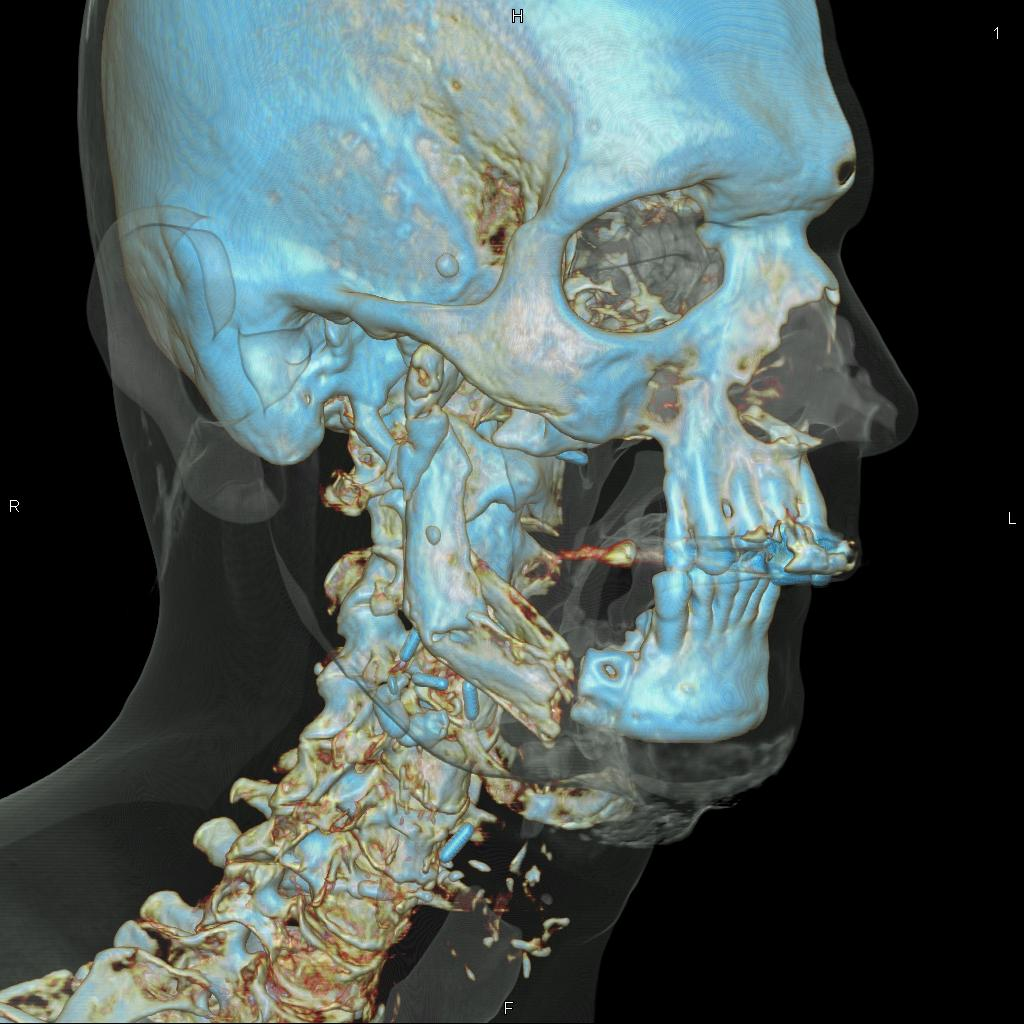
\includegraphics[width=0.85\linewidth]{images/head_vrt}
			\captionof{figure}{Volume rendering of a CT head scan. Image courtesy of Siemens AG.}%
			\label{fig:ct_intro_1}
		\end{minipage}% \hspace{1.3cm}
		\begin{minipage}{.45\linewidth}
			\centering
			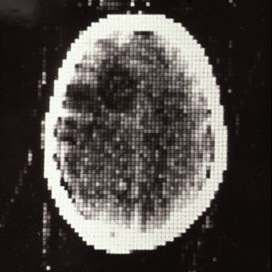
\includegraphics[width=0.85\linewidth]{images/first_clinical_ct_cut}
			\captionof{figure}{The first clinical CT scan, acquired October 1971 at Atkinson Morley's Hospital in London.}%
			\label{fig:ct_hist_1}
		\end{minipage}
	\end{figure}

\end{frame}

\subsection{Motivation}
\label{sub:ct_moti}

\begin{frame}
	\frametitle{Motivation}

	\begin{itemize}
		\item X-rays can be used to acquire 2-D projection images
		\item However, some spatial information is lost
		\item We only see ``shadows'' of the imaged objects
		\item But can we actually look ``inside''?
	\end{itemize}

\end{frame}

\begin{frame}
	\frametitle{Motivation}
	\begin{figure}[tb]
		\centering
		\begin{subfigure}[t]{0.375\linewidth}
			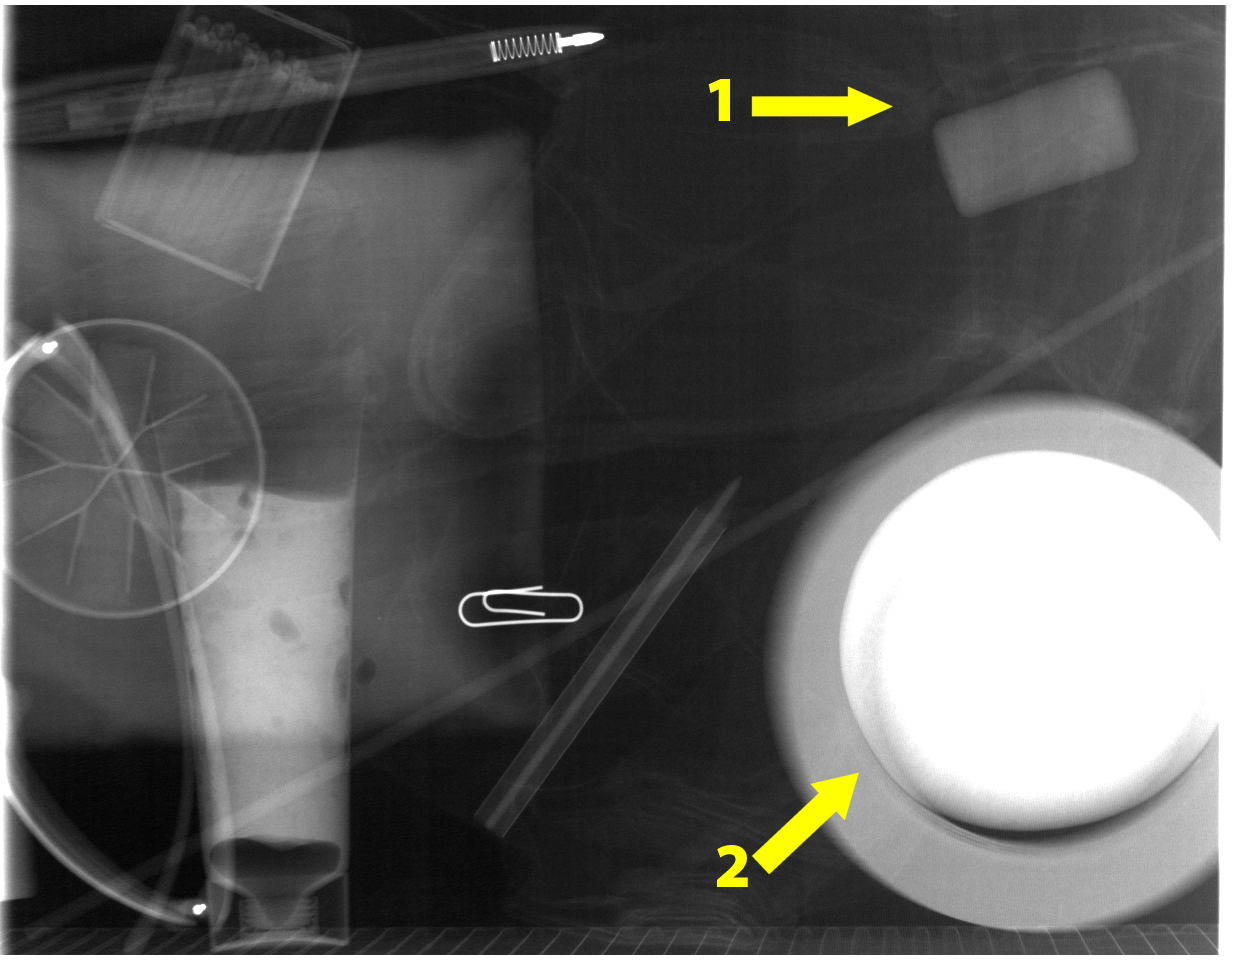
\includegraphics[width=\linewidth]{images/box_ann}
			\caption{}
			\label{fig:ct_mot_1.1}
		\end{subfigure}
		\begin{subfigure}[t]{0.29\linewidth}
			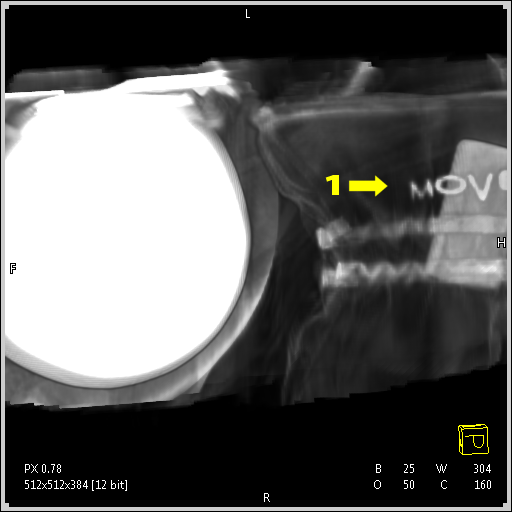
\includegraphics[width=\linewidth]{images/box_move}
			\caption{}
			\label{fig:ct_mot_1.2}
		\end{subfigure}
		\begin{subfigure}[t]{0.29\linewidth}
			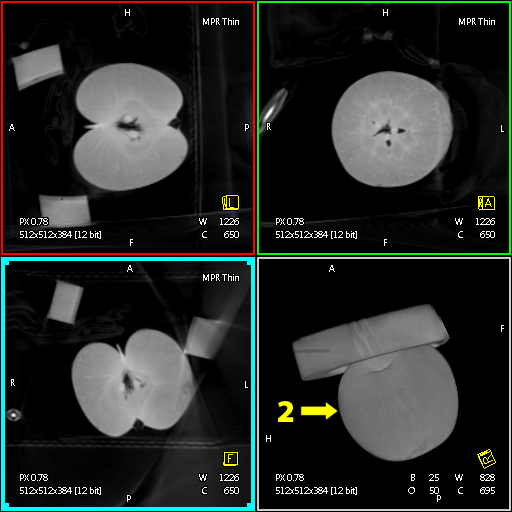
\includegraphics[width=\linewidth]{images/box_apple}
			\caption{}
			\label{fig:ct_mot_1.3}
		\end{subfigure}
		\caption{2-D X-ray projection image of a luggage bag \textbf{(a)} and a corresponding 3-D reconstruction, visualized with a volume rendering technique and \textbf{(b, c)} and as orthogonal cross-sectional slices \textbf{(c)}.}
		\label{fig:ct_mot_1}
	\end{figure}

\end{frame}


\subsection{Brief History}
\label{sub:ct_hist}

\begin{frame}{Brief History}

	\begin{itemize}
		\setlength\itemsep{0.3cm}
		\item \textcolor{faublue}{\textbf{1917:}} ``The determination of functions by their integrals along certain manifolds'' by Johann Radon -- no practical application for 50 years!
		\item \textcolor{faublue}{\textbf{1971:}} First CT built by Godfrey Hounsfield and Allan Cormack
		\item \textcolor{faublue}{\textbf{1979:}} Nobel prize in medicine awarded for this invention
		\item \textcolor{faublue}{\textbf{1990:}} Spiral (or rather: helical) CT by Willi Kalender et al.
		\item \textcolor{faublue}{\textbf{Early days of CT:}}\newline{} Approx.~$4$\,minutes per rotation, reconstruction of $80\times80$\,pixels at $3$\,bit depth took several hours
		\item \textcolor{faublue}{\textbf{2002:}} $0.4$\,seconds per rotation, up to $16$ slices in parallel, $512\times512$\,pixels at $16$\,bit depth reconstructed on-the-fly

	\end{itemize}

\end{frame}

\begin{frame}
	\frametitle{Brief History}

	\begin{itemize}
		\setlength\itemsep{0.3cm}
		\item \textcolor{faublue}{\textbf{2005:}} Dual source CT -- additional information from dual energy scans and faster regular acquisitions
		\item Multi-slice FOV up to $16$\,cm, sub-millimeter resolution -- complete organs in a single rotation!
		\item \textcolor{faublue}{\textbf{2014:}} Up to $128$ slices in parallel, temporal resolution $195$\,ms (single source)

	\end{itemize}

\end{frame}


\begin{frame}
	\frametitle{Brief History}

	\begin{figure}[tb]
		\centering
		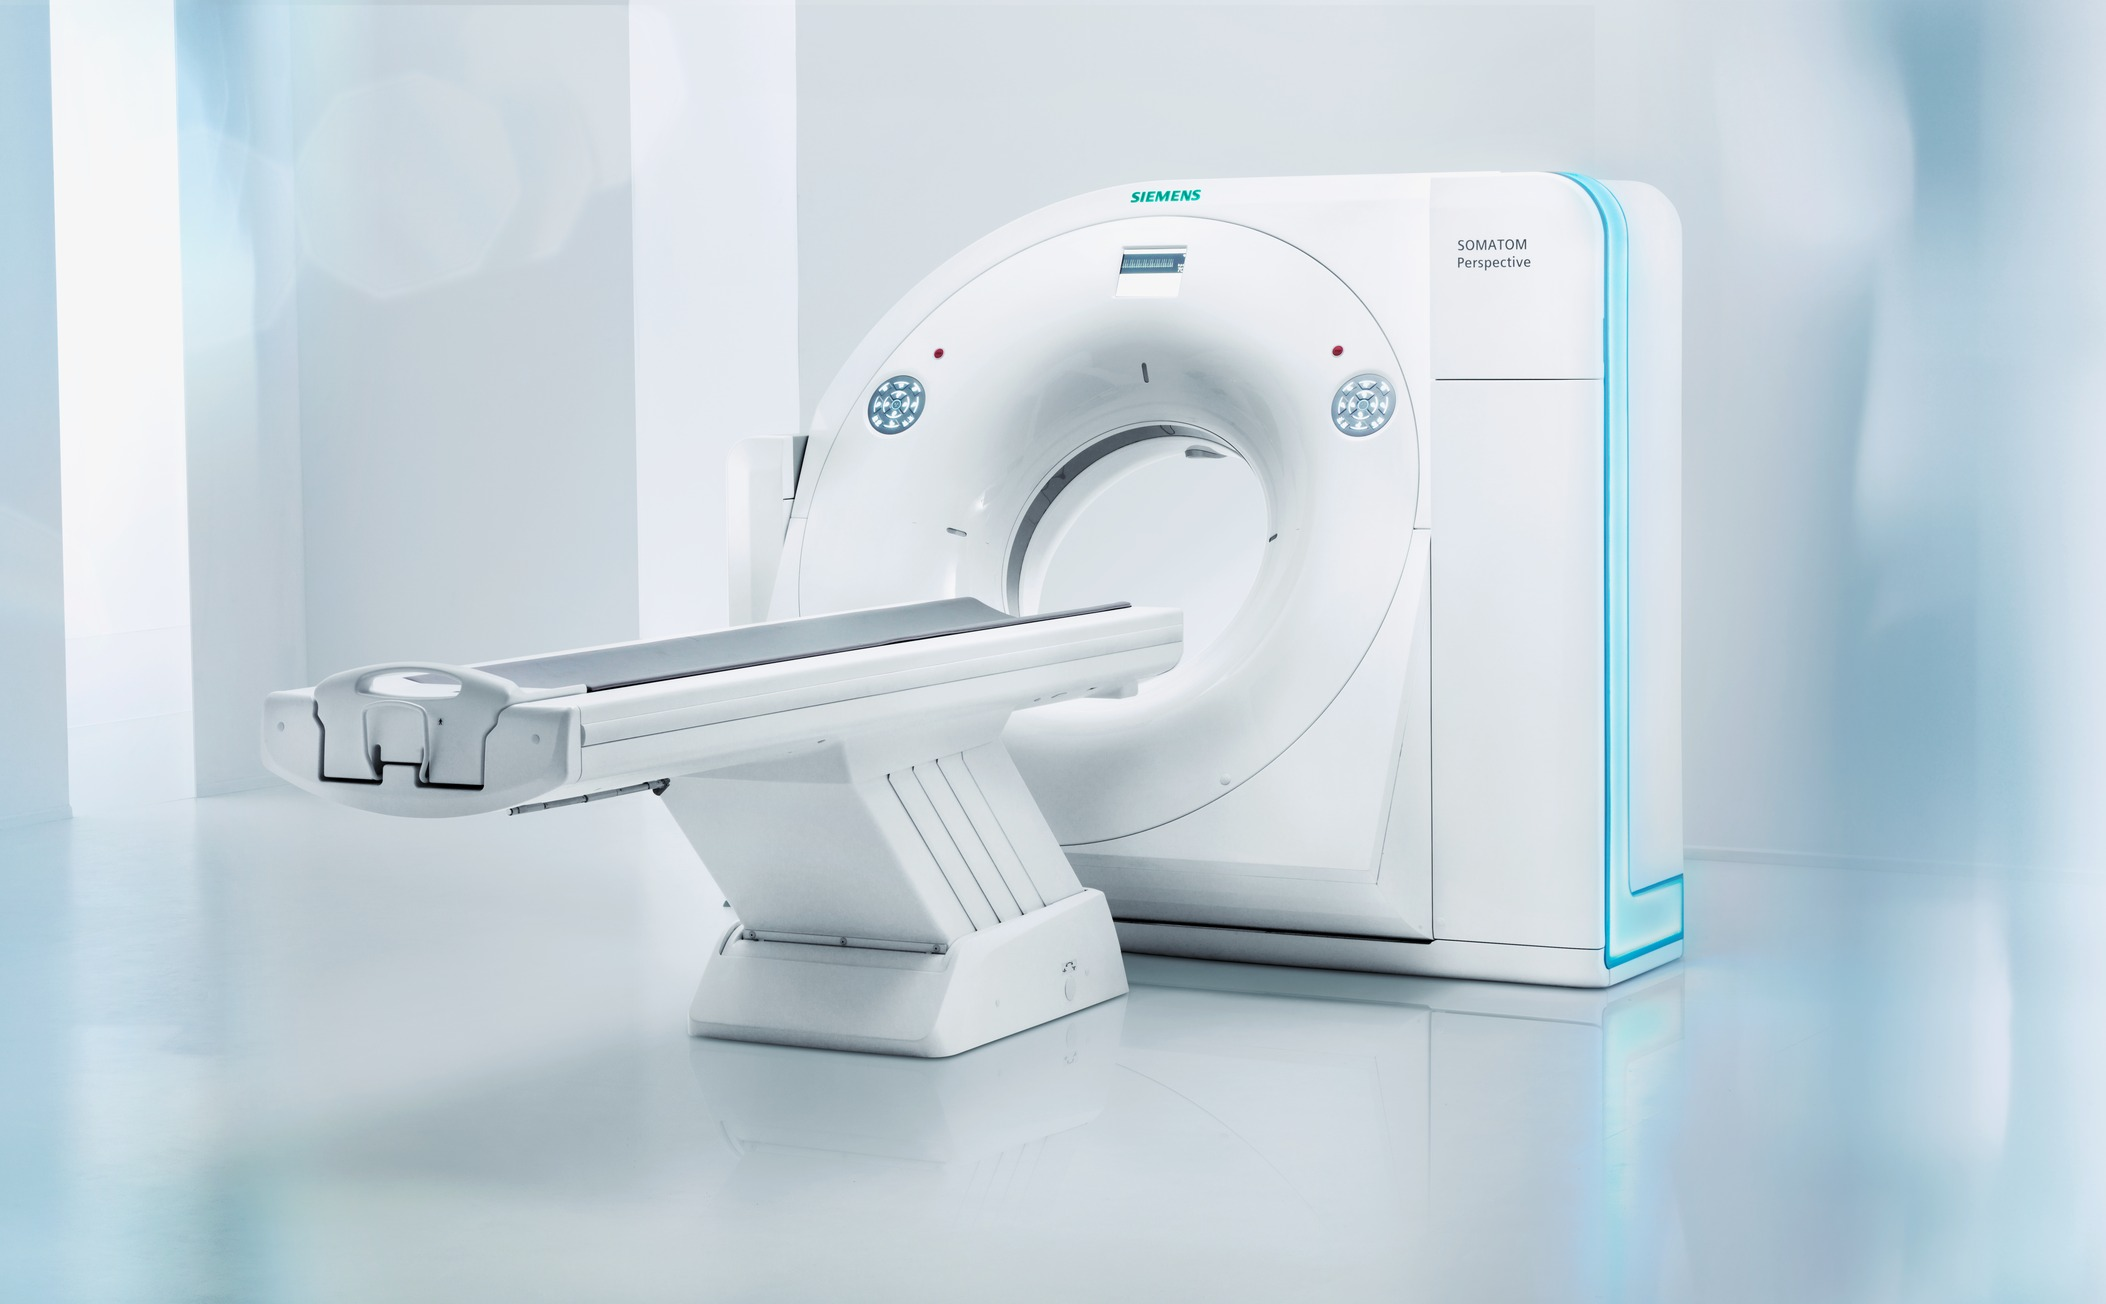
\includegraphics[height=0.75\textheight]{images/somatom_perspective}
		\caption{A modern CT scanner can acquire up to 128 image slices in parallel. Image courtesy of Siemens AG.}%
		\label{fig:ct_hist_2}
	\end{figure}

\end{frame}

\section{Mathematical Principles}%
\label{sec:ct_mat}

\begin{frame}
	\frametitle{Mathematical Principles}

	What will we cover?
	\vspace{0.3cm}

	\begin{itemize}
		\setlength\itemsep{0.3cm}
		\item Radon transform: Mathematical principle of image formation process
		\item Inverting this transform amounts to reconstruction
		\item Fourier slice theorem: Property related to the Radon transform
		\item Core idea of important reconstruction algorithms
	\end{itemize}

\end{frame}


\subsection{Radon Transform}%
\label{sub:ct_radon}

\begin{frame}{Recap: X-Ray}
    $I_0$: Incident X-ray intensity. \\
    $I$: Detected X-ray intensity.
    \vskip12pt
    \bluefat{Lambert-Beer's Law}:\\
    \begin{center}
     \vskip6pt
        $I=I_0\cdot e^{-\int \mu d\ell}$\\

   \end{center}

 \end{frame}
    
 \begin{frame}{Recap: X-Ray}
    $I_0$: Incident X-ray intensity. \\
    $I$: Detected X-ray intensity.
    \vskip12pt
    \bluefat{Lambert-Beer's Law}:\\
    \begin{center}
     \vskip6pt
        $I=I_0\cdot e^{-\int \mu d\ell}$\\
        \vskip6pt
        $I=I_0\cdot e^{-\int f(\ell) d\ell}$\\
    \end{center}

	\begin{figure}[tbp]
		\centering
		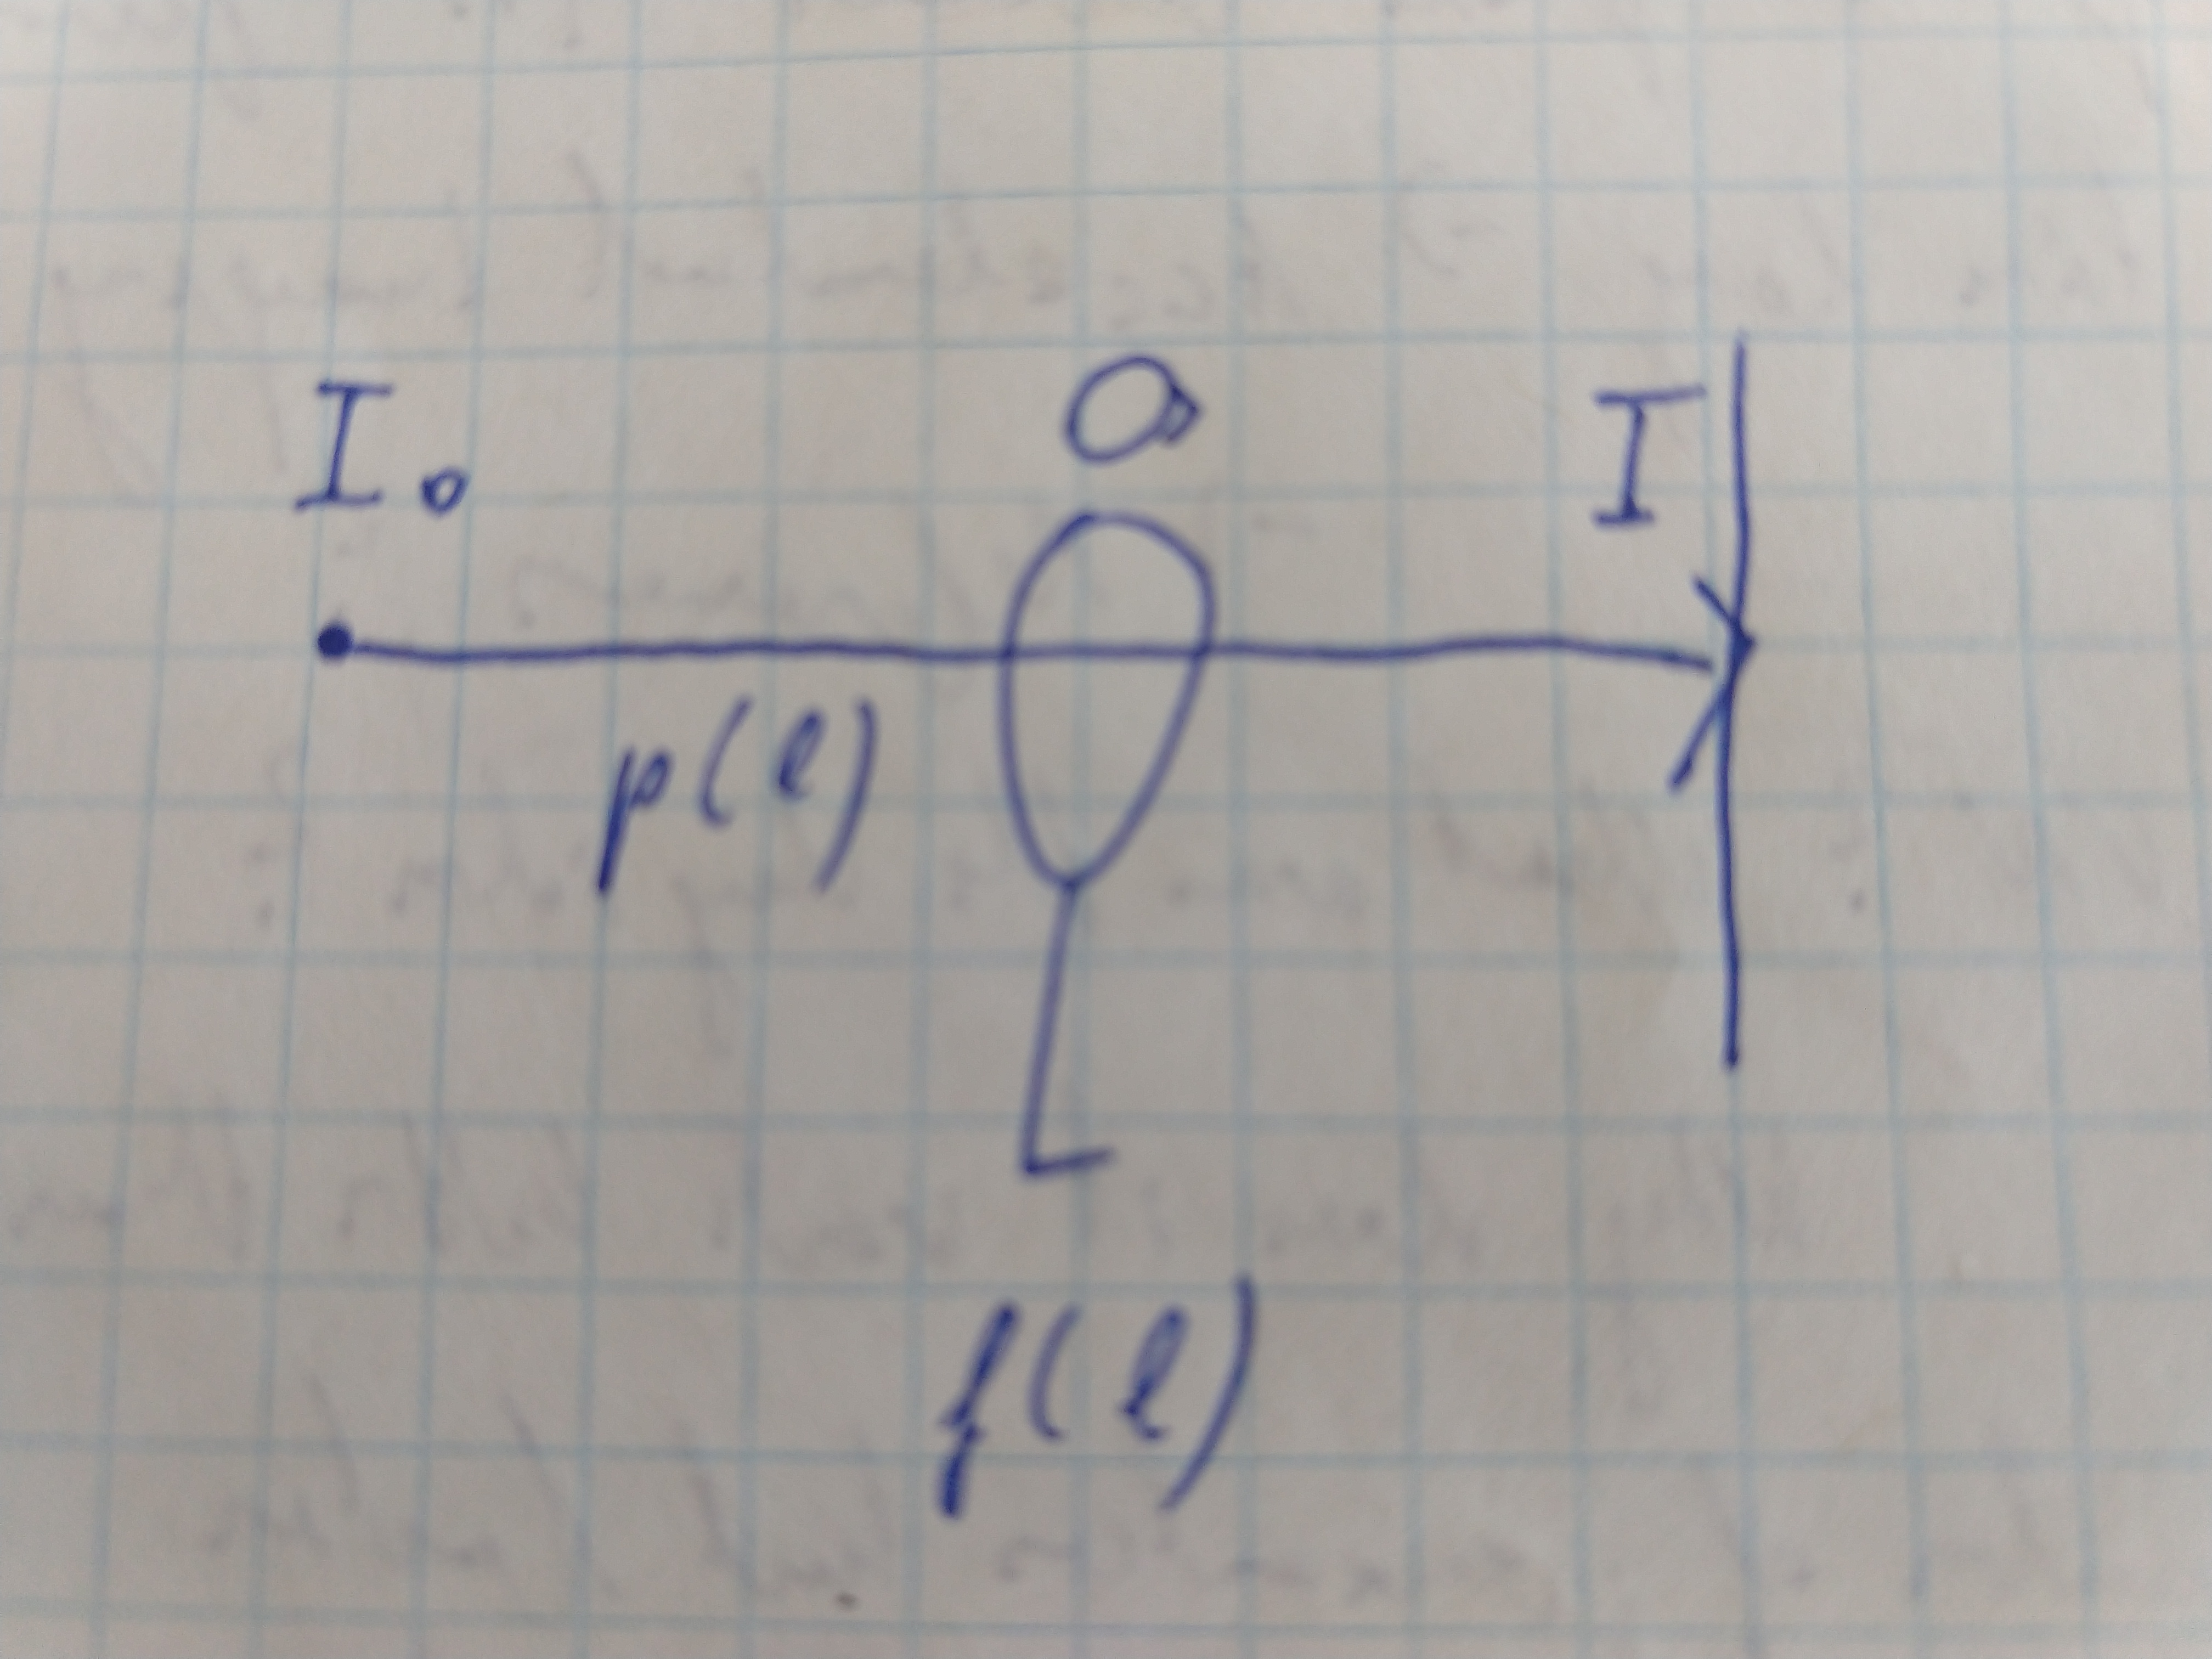
\includegraphics[height=0.3\textheight]{images/x_ray_sketch}
		\label{fig:x_ray_sketch}
	\end{figure}
 \end{frame}

 \begin{frame}{Recap: X-Ray}
    $I_0$: Incident X-ray intensity. \\
    $I$: Detected X-ray intensity.
    \vskip12pt
    \bluefat{Lambert-Beer's Law}:\\
    \begin{center}
     \vskip6pt
        $I=I_0\cdot e^{-\int \mu d\ell}$\\
        \vskip6pt
        $I=I_0\cdot e^{-\int f(\ell) d\ell}$\\
        \vskip6pt
        $-ln \frac{I}{I_0} = \int f(\ell) d\ell$
    \end{center}

	\begin{figure}[tbp]
		\centering
		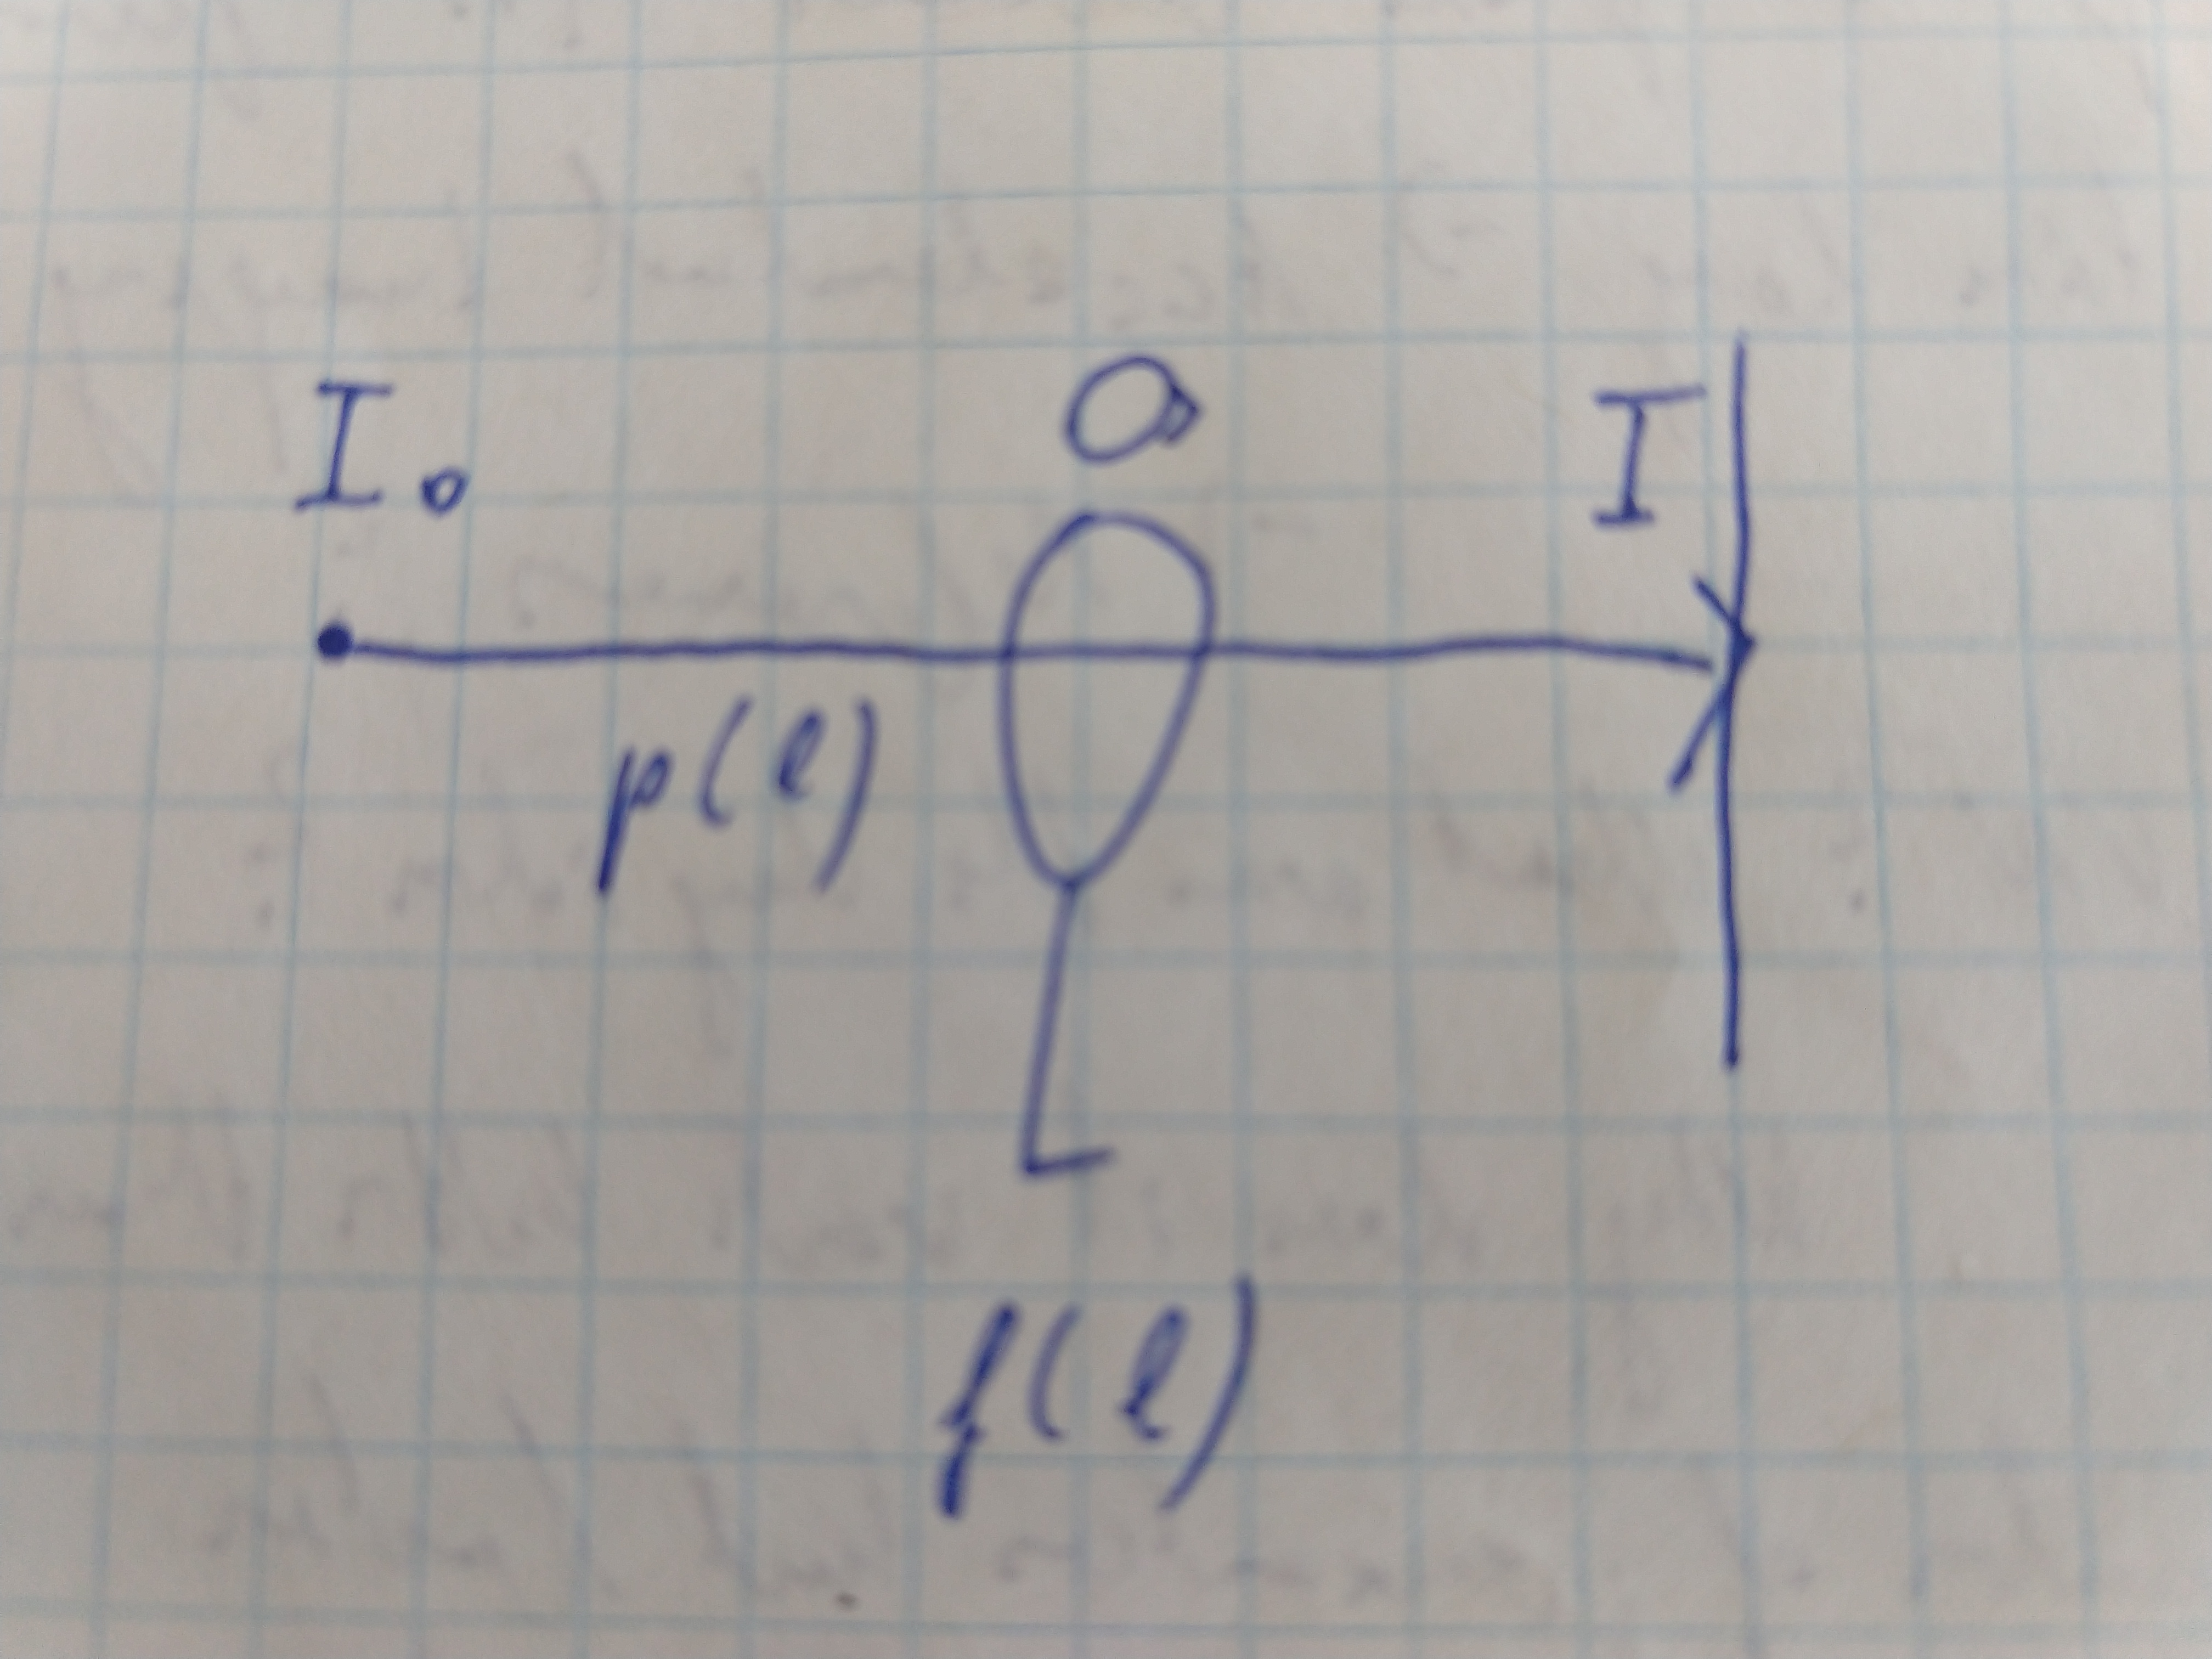
\includegraphics[height=0.3\textheight]{images/x_ray_sketch}
		\label{fig:x_ray_sketch}
	\end{figure}	
 \end{frame}
 
  \begin{frame}{Recap: X-Ray}
    $I_0$: Incident X-ray intensity. \\
    $I$: Detected X-ray intensity.
    \vskip12pt
    \bluefat{Lambert-Beer's Law}:\\
    \begin{center}
     \vskip6pt
        $I=I_0\cdot e^{-\int \mu d\ell}$\\
        \vskip6pt
        $I=I_0\cdot e^{-\int f(\ell) d\ell}$\\
        \vskip6pt
        $-ln \frac{I}{I_0} = \int f(\ell) d\ell := p(\ell)$
    \end{center}

	\begin{figure}[tbp]
		\centering
		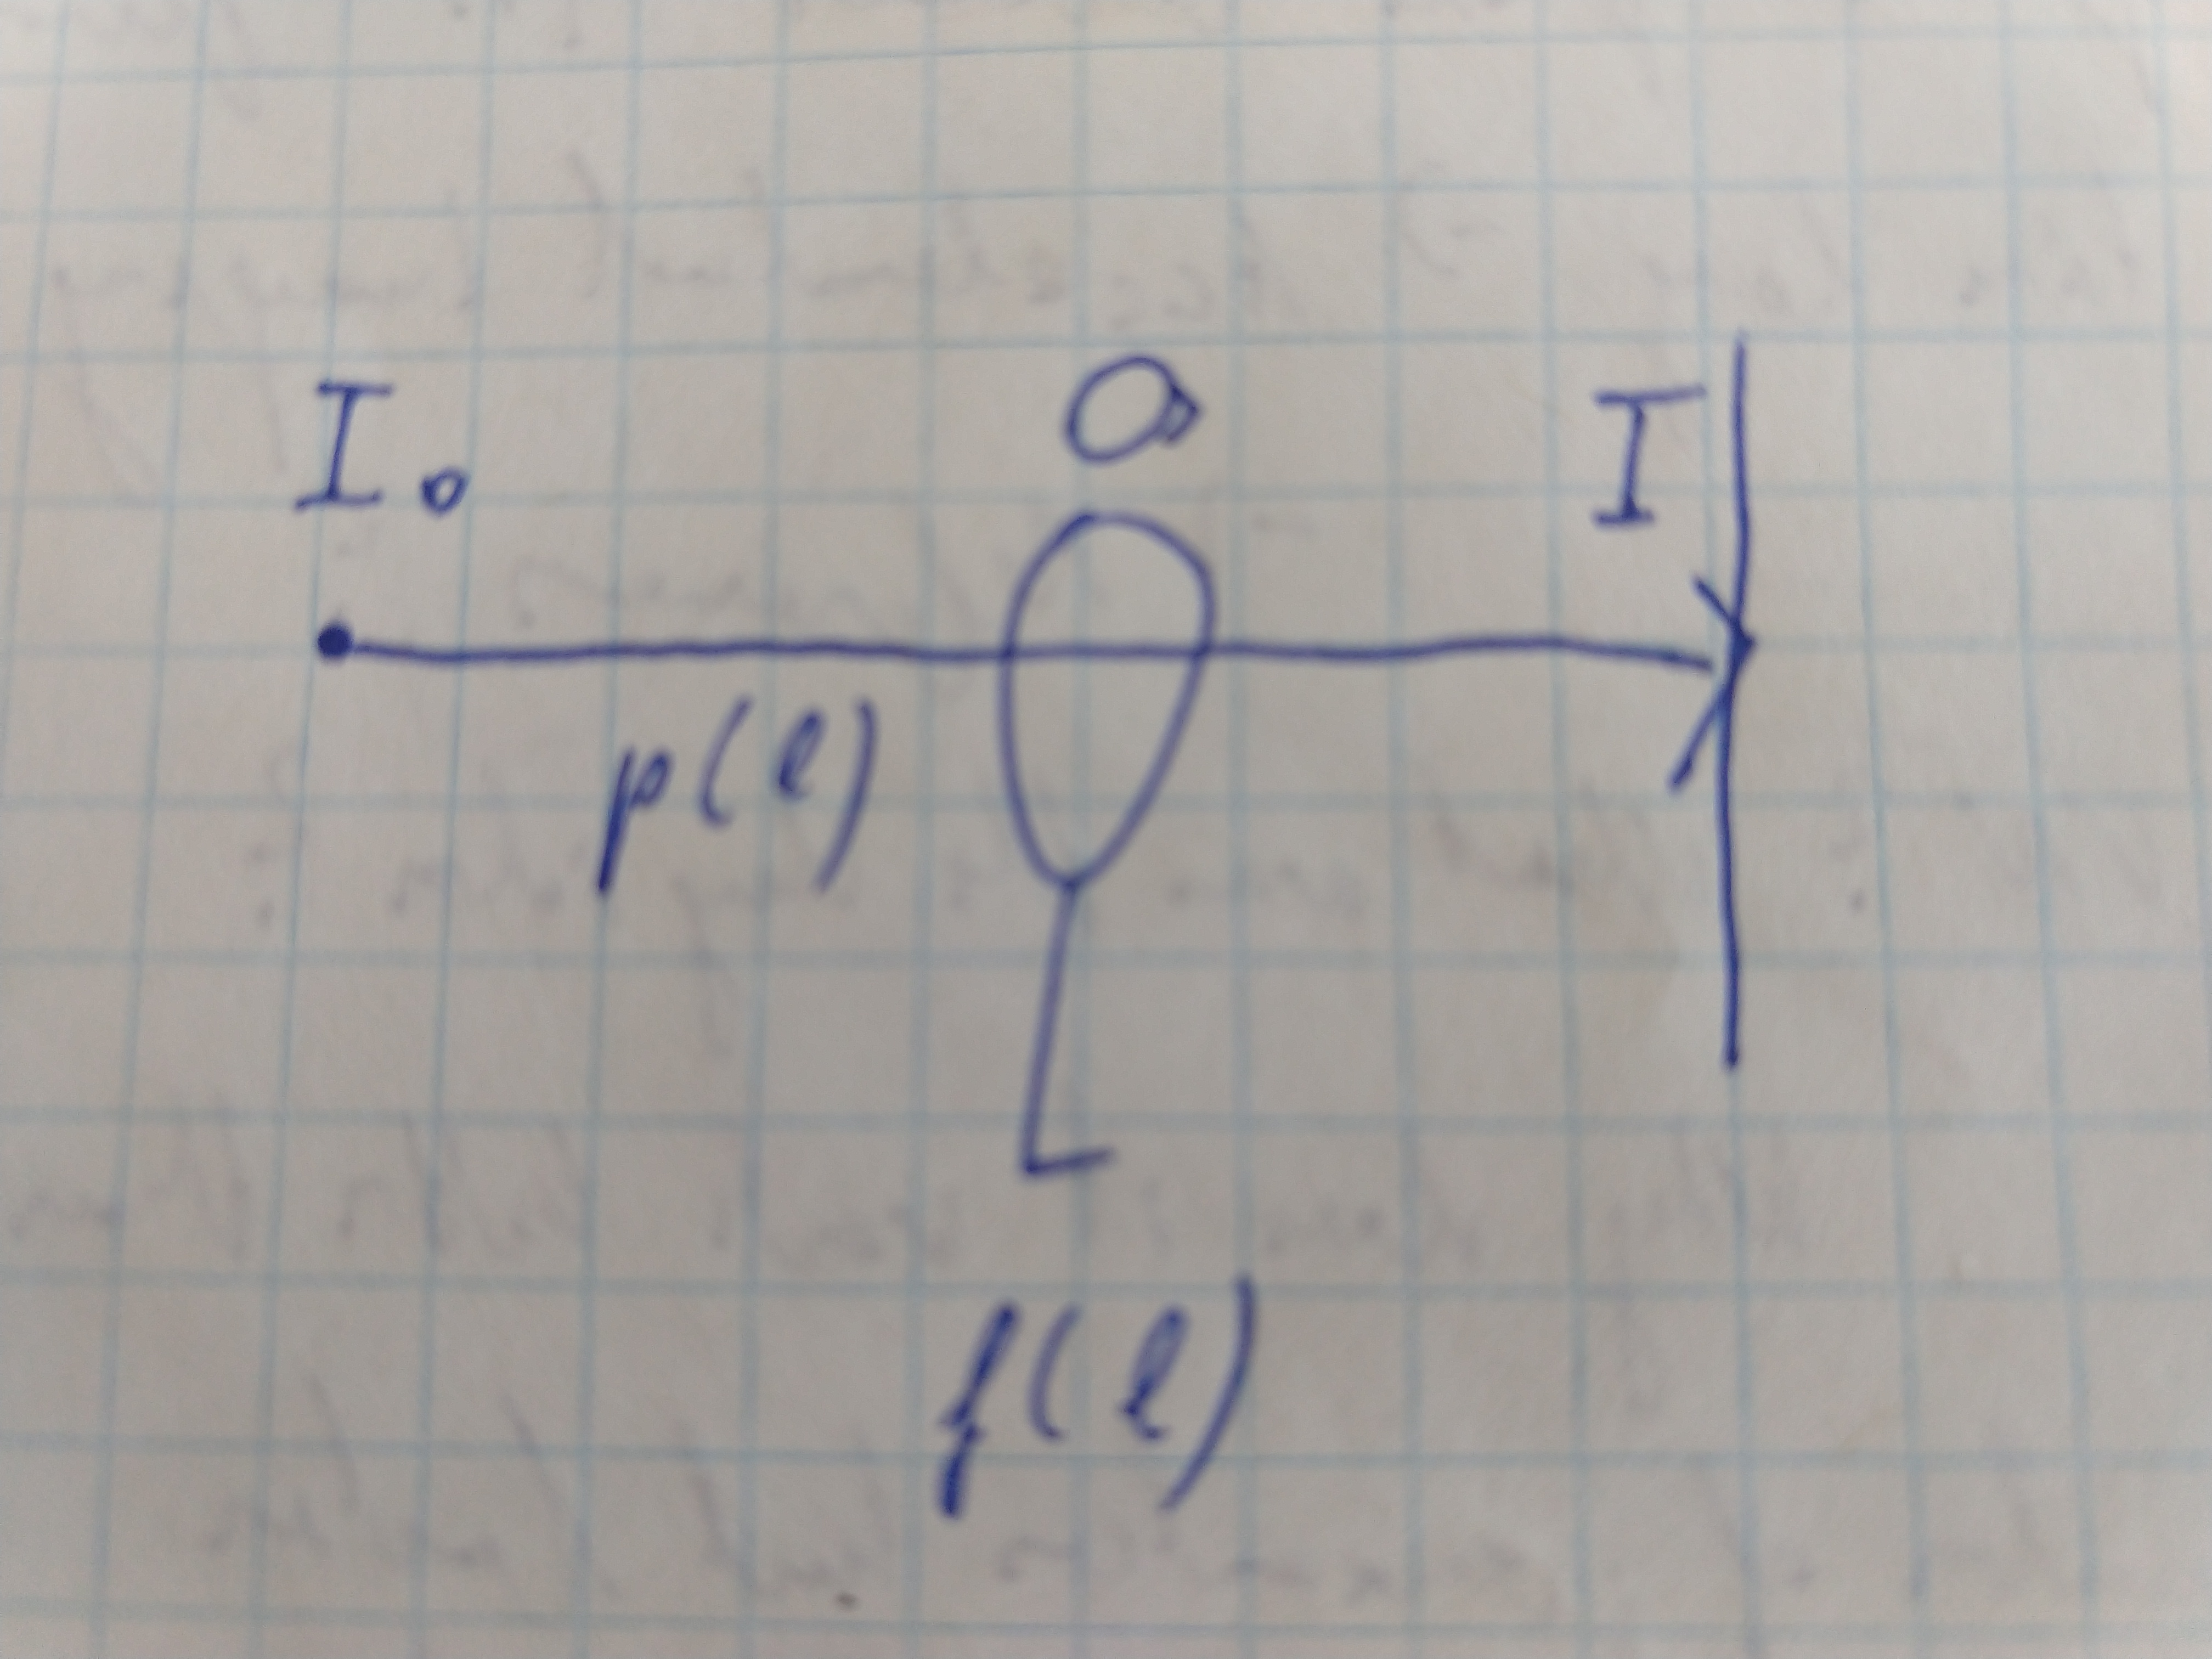
\includegraphics[height=0.3\textheight]{images/x_ray_sketch}
		\label{fig:x_ray_sketch}
	\end{figure}	
 \end{frame}

 
\begin{frame}
	\frametitle{Radon Transform}

	Radon's key insight: Any integrable function $f(x,y)$ can be uniquely represented by -- and therefore recovered from -- all straight line integrals over its domain,

	\begin{equation}
		\label{eqn:ct_radon_1}
		p(\ell) = \int_{-\infty}^{+\infty} f\left(x\left(l\right), y\left(l\right)\right) \ \text{d}l, \quad \forall l: \left(x\left(l\right), y\left(l\right)\right)^\top \in \text{line } \ell
	\end{equation}
		
	\begin{figure}[tbp]
		\centering
		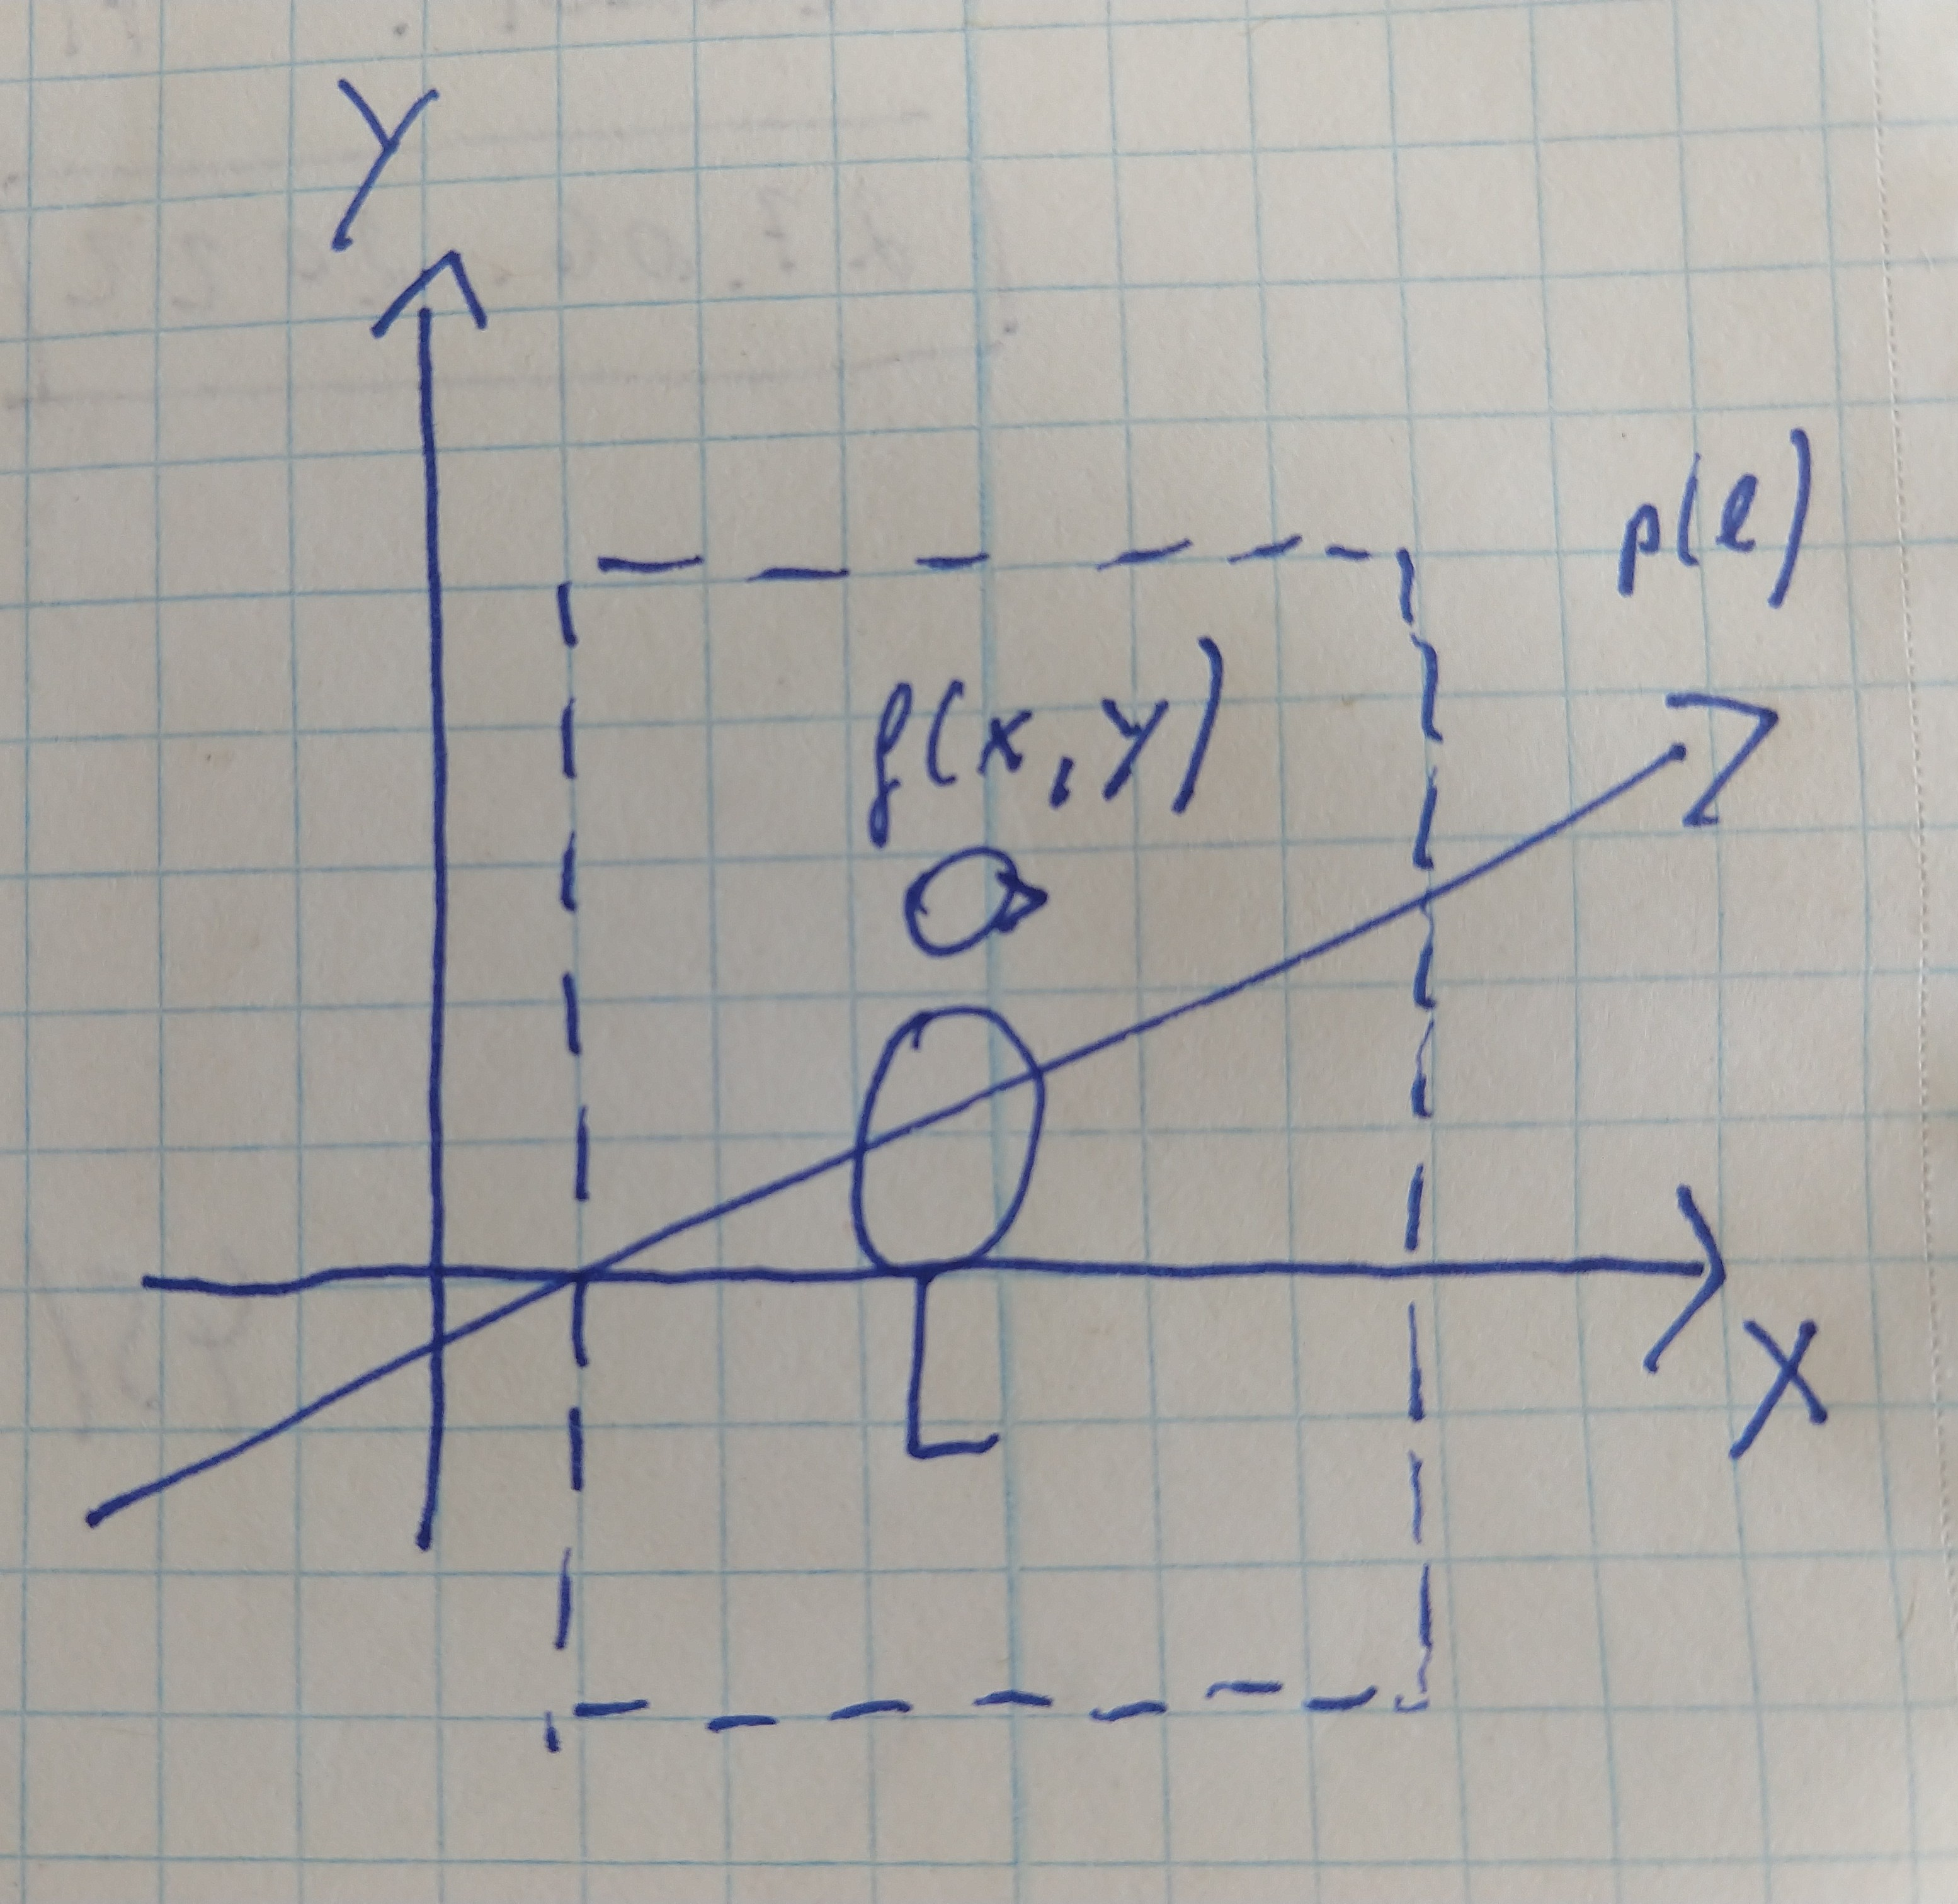
\includegraphics[height=0.4\textheight]{images/radon1_sketch}%
		\label{fig:ct_radon1_sketch}
	\end{figure}
	
\end{frame}



\begin{frame}
	\frametitle{Radon Transform}
	How to describe each line uniquely? In terms of polar coordinates:

	\begin{equation}
		\label{eqn:ct_radon_2}
		p(\theta, s) =\iint_{-\infty}^{+\infty} f(x,y) \delta\left(x \cos \theta + y \sin \theta - s\right) \ \textnormal{d}x\textnormal{d}y,
	\end{equation}

	\begin{columns}[c, onlytextwidth]
		\begin{column}{0.5\textwidth}
			\begin{figure}[tbp]
				\centering
				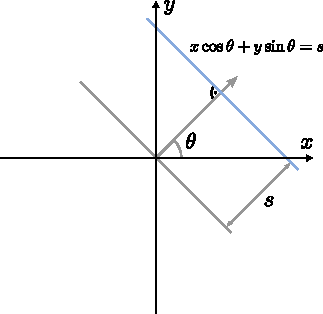
\includegraphics[height=0.6\textheight]{images/radon_1}%
				\label{fig:ct_radon_1}
			\end{figure}
		\end{column}\begin{column}{0.5\textwidth}
			\begin{itemize}
				\setlength\itemsep{0.3cm}
				\item Distance to origin $s$
				\item Angle $\theta$
				\item[$\Rightarrow$] Line equation:
				      \begin{equation}
					      x \cos{\theta} + y \sin{\theta} = s
				      \end{equation}
			\end{itemize}
		\end{column}
	\end{columns}

\end{frame}

\begin{frame}
	\frametitle{Radon Transform}

	\begin{itemize}
		\setlength\itemsep{0.3cm}
		\item Complete set of line integrals obtained for $\theta \in [0^\circ, 180^\circ]$ and $s \in [-\infty, +\infty]$
		\item $p_{\theta}(s) = p(\theta,s)$ is called a projection
		\item Contains all line integrals for a constant $\theta$ and variable distance $s$
		\item Turning $f(x,y)$ into line integral values $p(\theta, s)$ is the Radon transform
		\item Reconstruction computes the inverse, i.\,e.~$f(x,y)$ from line integrals
	\end{itemize}

	\begin{figure}[tbp]
		\centering
		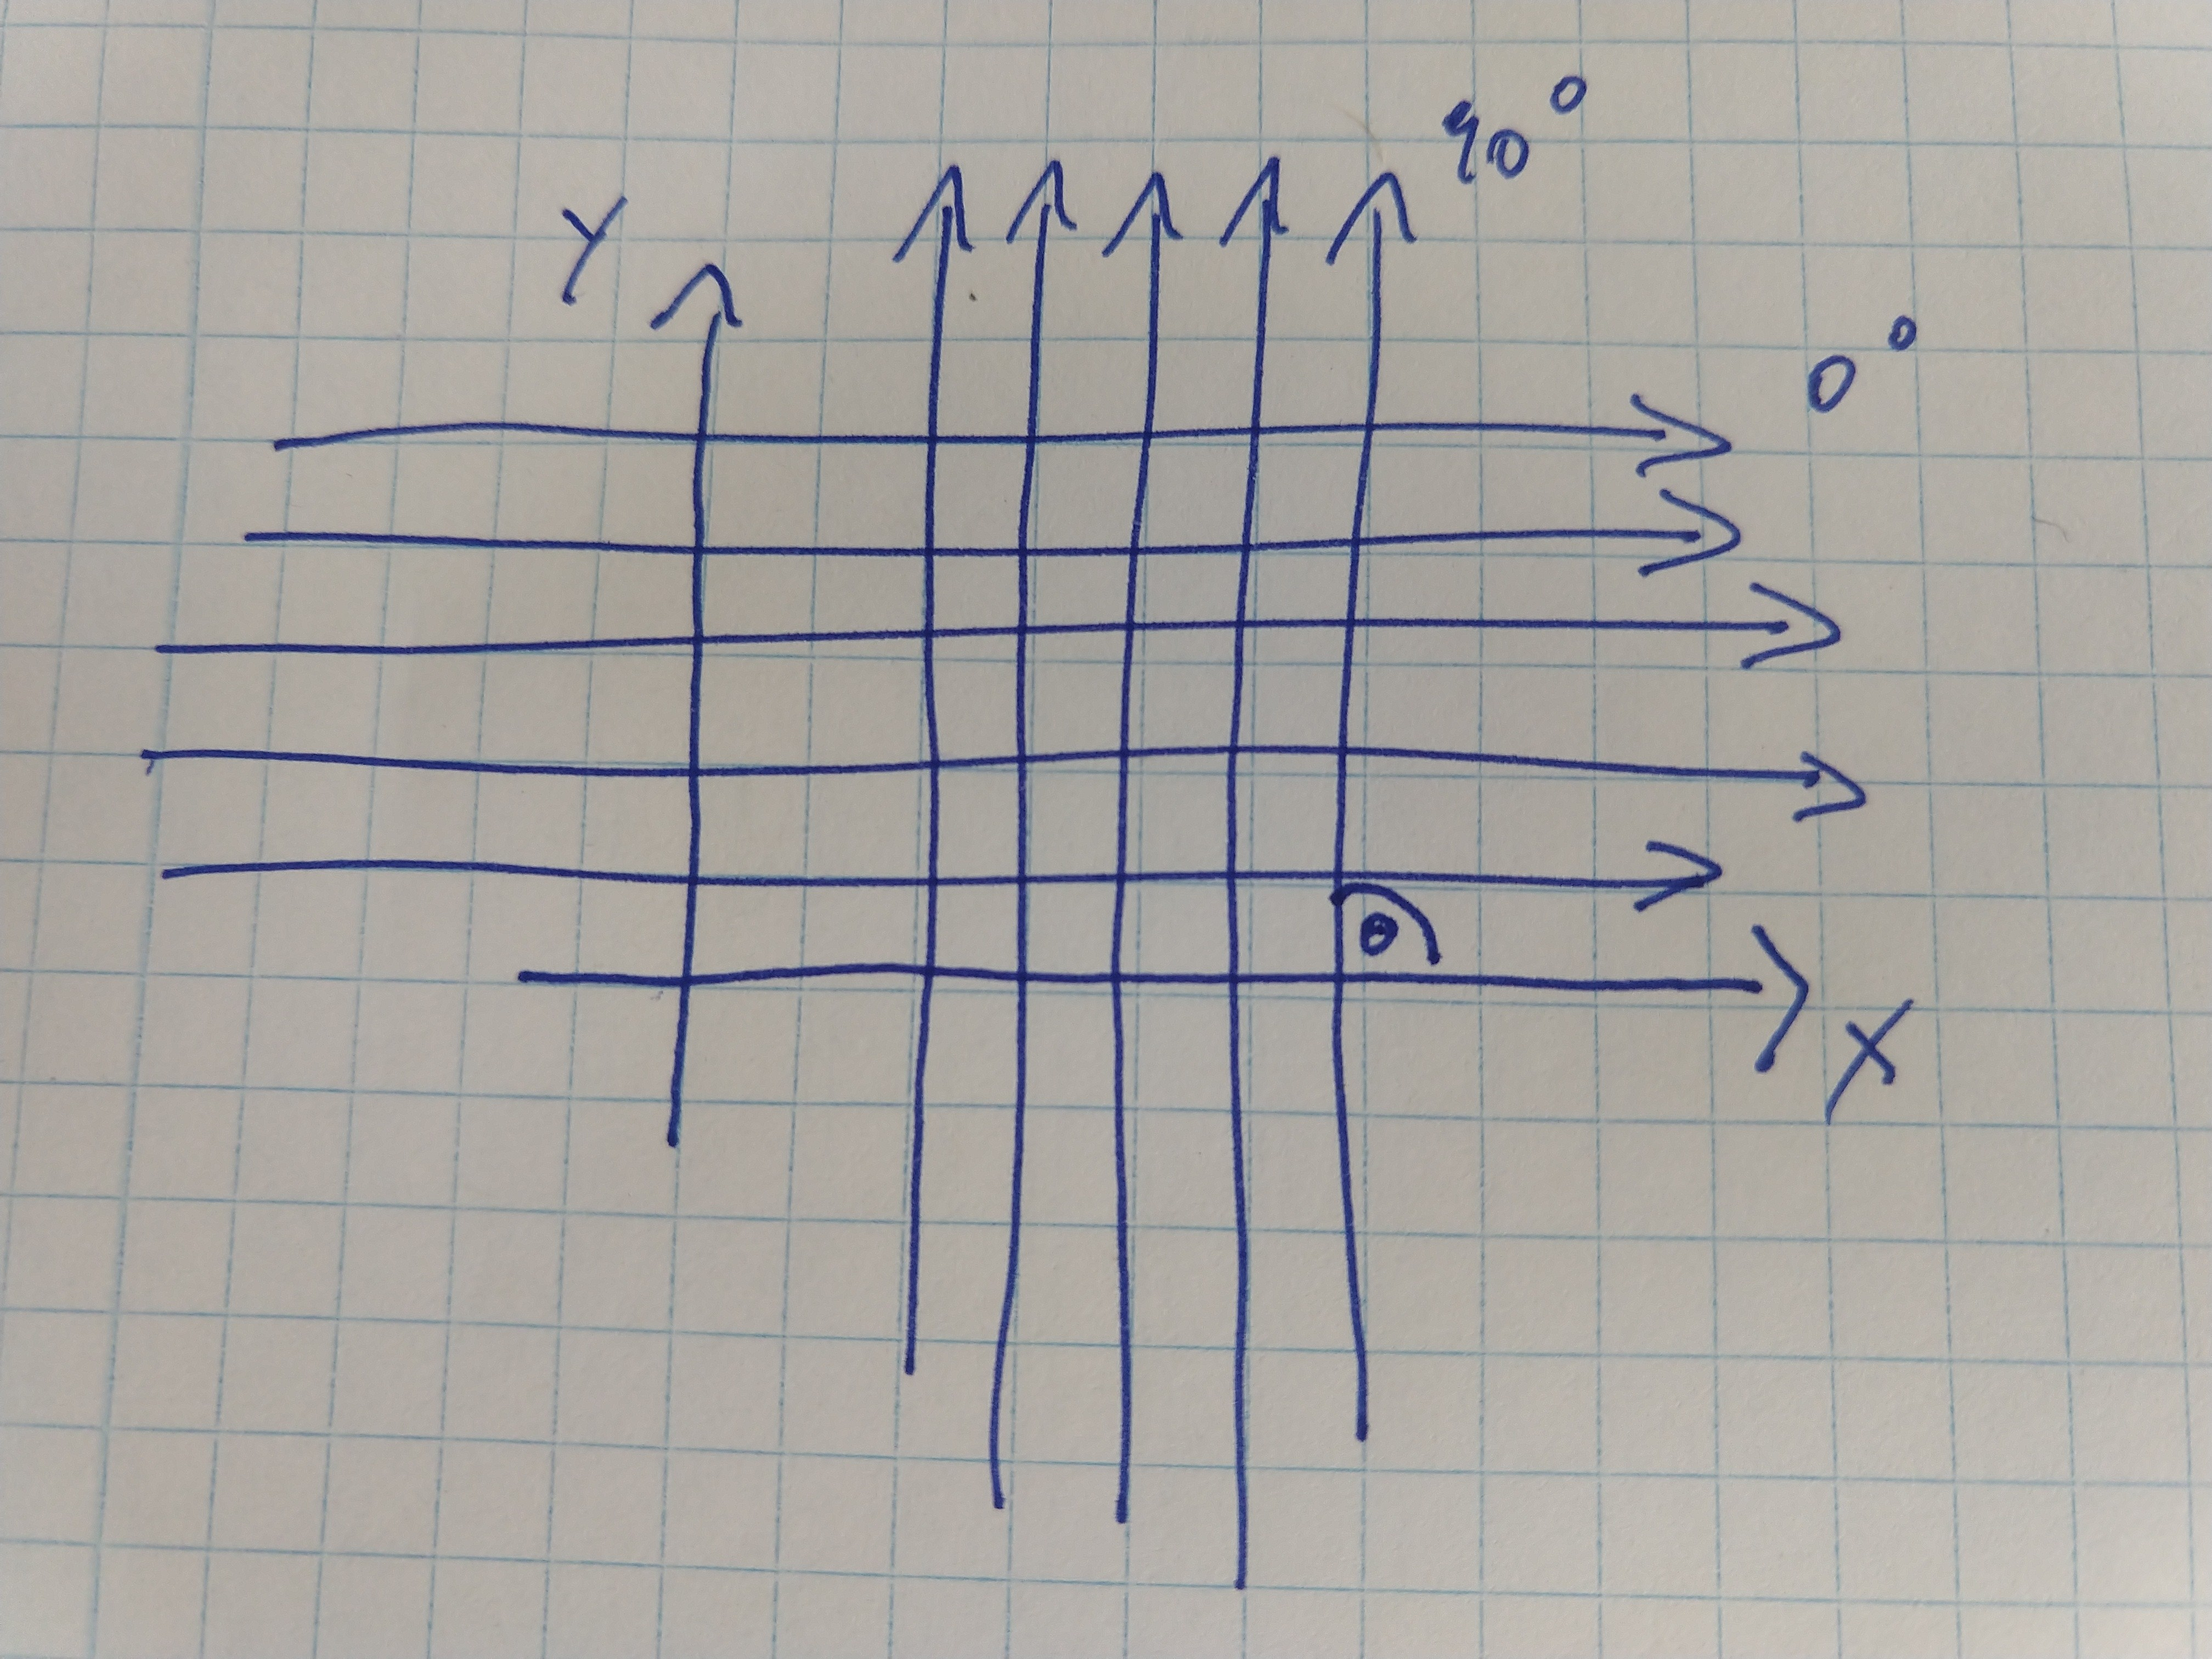
\includegraphics[height=0.4\textheight]{images/radon2_rotation}%
		\label{fig:ct_radon2_rotation}
	\end{figure}
	
\end{frame}

\begin{frame}
	\frametitle{Sinogram}

	Arranging projections as a 2-D image yields the sinogram, named for the sinusoidal curves emerging from the underlying geometry.

	\begin{figure}[tbp]
		\centering
		\includegraphics[width=0.75\linewidth]{images/radon_2}
		\caption{$f(x, y)$ has a constant non-zero value inside the blue circle and vanishes everywhere else. We see a single projection on the left and where it fits into the whole sinogram on the right.}%
		\label{fig:ct_radon_2}
	\end{figure}

\end{frame}

\subsection{Fourier Slice Theorem}%
\label{sub:ct_fourier}

\begin{frame}
	\frametitle{Fourier Slice Theorem}

	Let's consider frequency domain representations of $p_\theta(s)$ and $f(x, y)$,

	\begin{eqnarray}
		F(u,v) &=& \mathcal{F}\left\{f(x,y)\right\},\\
		P_{\theta}(\omega) &=& \mathcal{F}\left\{p_\theta(s)\right\},
	\end{eqnarray}
	using the Fourier transform $\mathcal{F}$.\\[1cm]

	We can find a relationship between both, known as the Fourier Slice Theorem (FST):
	$P_{\theta}(\omega)$ is equivalent to the part of $F(u,v)$ that falls on a radial line with angle $\theta$.
\end{frame}

\begin{frame}
	\frametitle{Fourier Slice Theorem}

	%%
	\begin{figure}[tbp]
		\centering
		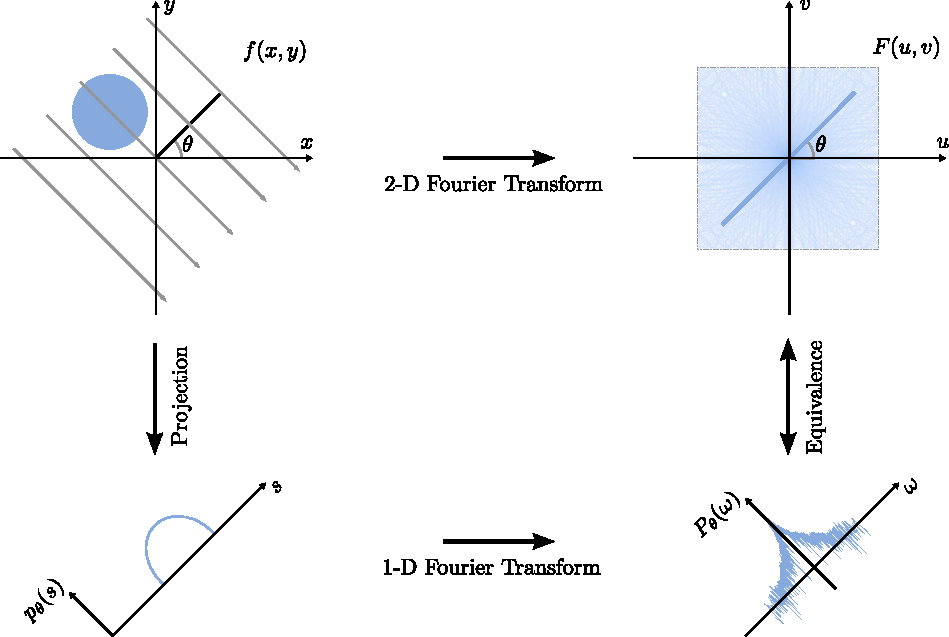
\includegraphics[width=0.6\linewidth]{images/fourier_1}
		%       \caption{The Fourier slice theorem establishes an equivalence between the Fourier transform $P_\theta(\omega)$ of the projection $p_\theta(s)$ and a line in the Fourier transform $F(u, v)$ of $f(x,y)$ which runs through the origin and forms the angle $\theta$ with the $u$-axis. Please note that in the frequency domain images on the right, the magnitudes of the complex numbers were plotted on a logarithmic scale for improved readability.}
		\label{fig:ct_fourier_1}
	\end{figure}
	%

\end{frame}

%\begin{frame}[allowframebreaks]
%\frametitle{Fourier Slice Theorem}
%
%Proof:
%
%\begin{itemize}
%
%\item Write down definition of $P_{\theta}(\omega)$:
%\begin{equation}
%P_{\theta}(\omega) = \int_{-\infty}^{+\infty} p_\theta(s) e^{-2\pi i\omega s} \ \textnormal{d}s 
%\end{equation}
%
%\item Insert definition of $p_\theta(s)$:
%\begin{equation}
%P_{\theta}(\omega) = \int_{-\infty}^{+\infty} \iint_{-\infty}^{+\infty} f(x,y) \delta(x \cos \theta + y \sin \theta - s) \ \textnormal{d}x\textnormal{d}y \ e^{-2\pi i \omega s} \ \textnormal{d}s
%\end{equation}
%
%\item Rearrange integrals:
%\begin{equation}
%P_{\theta}(\omega) = \iint_{-\infty}^{+\infty} f(x,y) \int_{-\infty}^{+\infty}  \delta(x \cos \theta + y \sin \theta - s) e^{-2\pi i \omega s} \ \textnormal{d}s\textnormal{d}x \textnormal{d}y
%\end{equation}
%
%\item Eliminate delta:
%\begin{equation}
%P_{\theta}(\omega) = \iint_{-\infty}^{+\infty} f(x,y) e^{-2\pi i (x \cos \theta + y \sin \theta)\omega} \ \textnormal{d}x \textnormal{d}y
%\end{equation}
%
%\item Substitute variables:
%\begin{equation}
%P_{\theta}(\omega) = \iint_{-\infty}^{+\infty} f(x,y) e^{-2\pi i (x u+ y v)} |_{u=\omega \cos \theta, \ v = \omega \sin \theta} \ \textnormal{d}x \textnormal{d}y
%\end{equation}
%
%\item This is the 2-D Fourier transform:
%\begin{equation}
%P_{\theta}(\omega) = F(\omega \cos \theta, \omega \sin \theta) = F_{\textnormal{polar}}(\omega, \theta)
%\end{equation}
%
%\end{itemize}
%
%$\Rightarrow$ By varying $\theta$, we can get the 2-D Fourier transform of $f(x,y)$ in polar coordinates $(\omega, \theta)$!
%
%\end{frame}

\begin{frame}
	\frametitle{Recall from MR Imaging: 2-D $\vec k$-Space}

	\begin{itemize}
		\item 2-D $\vec k$-space with phase patterns associated with some positions:
	\end{itemize}

	\vspace{-2ex}

	\begin{center}
		\newlength\imagewidth
\newlength\imagescale
\pgfmathsetlength{\imagewidth}{0.3\linewidth}
\pgfmathsetlength{\imagescale}{\imagewidth/128}
\tikzsetnextfilename{mr_k_space}
\begin{tikzpicture}[x=\imagescale,y=-\imagescale]
	\node[anchor=north west,inner sep=0pt,outer sep=0pt] (ksp) at (-0.5,-0.5)
   {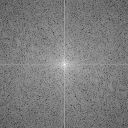
\includegraphics[width=\imagewidth]{images/kspace}};
	\draw[thick,->] (-4, 64) -- (131, 64) node [right] {$k_x$};
	\draw[thick,->] (64, 131) -- (64, -4) node [above] {$k_y$};
	\filldraw (64, 54) coordinate (ksp1) circle (1.5pt);
	\filldraw (69, 64) coordinate (ksp2) circle (1.5pt);
	\filldraw (60, 56) coordinate (ksp3) circle (1.5pt);
	\filldraw (54, 79) coordinate (ksp4) circle (1.5pt);
	
	\node[anchor=north west,inner sep=0pt,outer sep=0pt] (kspf1) at ($(ksp.north east) + (1cm, 0)$) {
\includegraphics[width=.1509\linewidth]{images/spatialfreq_0_10}};
	\draw[->, shorten >=1mm] (ksp1) -- (kspf1.west);
	\node[anchor=south west,inner sep=0pt,outer sep=0pt] (kspf2) at ($(ksp.south east) + (1cm, 0)$) {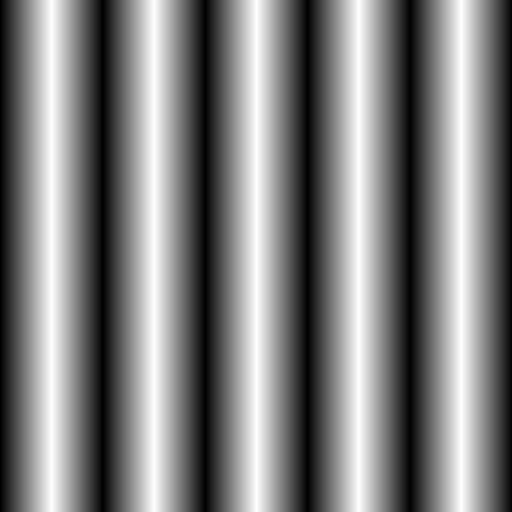
\includegraphics[width=.1509\linewidth]{images/spatialfreq_5_0}};
	\draw[->, shorten >=1mm] (ksp2) -- (kspf2.west);
	\node[anchor=north east,inner sep=0pt,outer sep=0pt] (kspf3) at ($(ksp.north west) - (1cm, 0)$) {\reflectbox{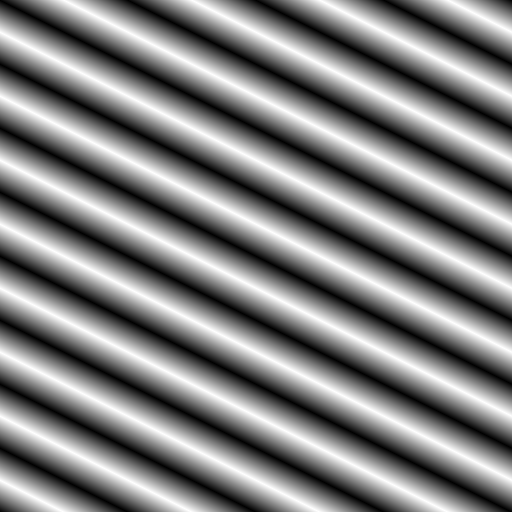
\includegraphics[width=.1509\linewidth]{images/spatialfreq_-4_8}}};
	\draw[->, shorten >=1mm] (ksp3) -- (kspf3.east);
	\node[anchor=south east,inner sep=0pt,outer sep=0pt] (kspf4) at ($(ksp.south west) - (1cm, 0)$) {\reflectbox{
\includegraphics[width=.1509\linewidth]{images/spatialfreq_-10_-15}}};
	\draw[->, shorten >=1mm] (ksp4) -- (kspf4.east);
\end{tikzpicture}

	\end{center}
\end{frame}

\begin{frame}
	\frametitle{Fourier Slice Theorem --- Graphical Explanation}
	\centering
	\def\svgwidth{0.55\linewidth}
	\input{images/GrahpicalFourierSliceTheorem.pdf_tex}

\end{frame}

\begin{frame}[c]{Fourier Slice Theorem --- Graphical Explanation}
	\centering
	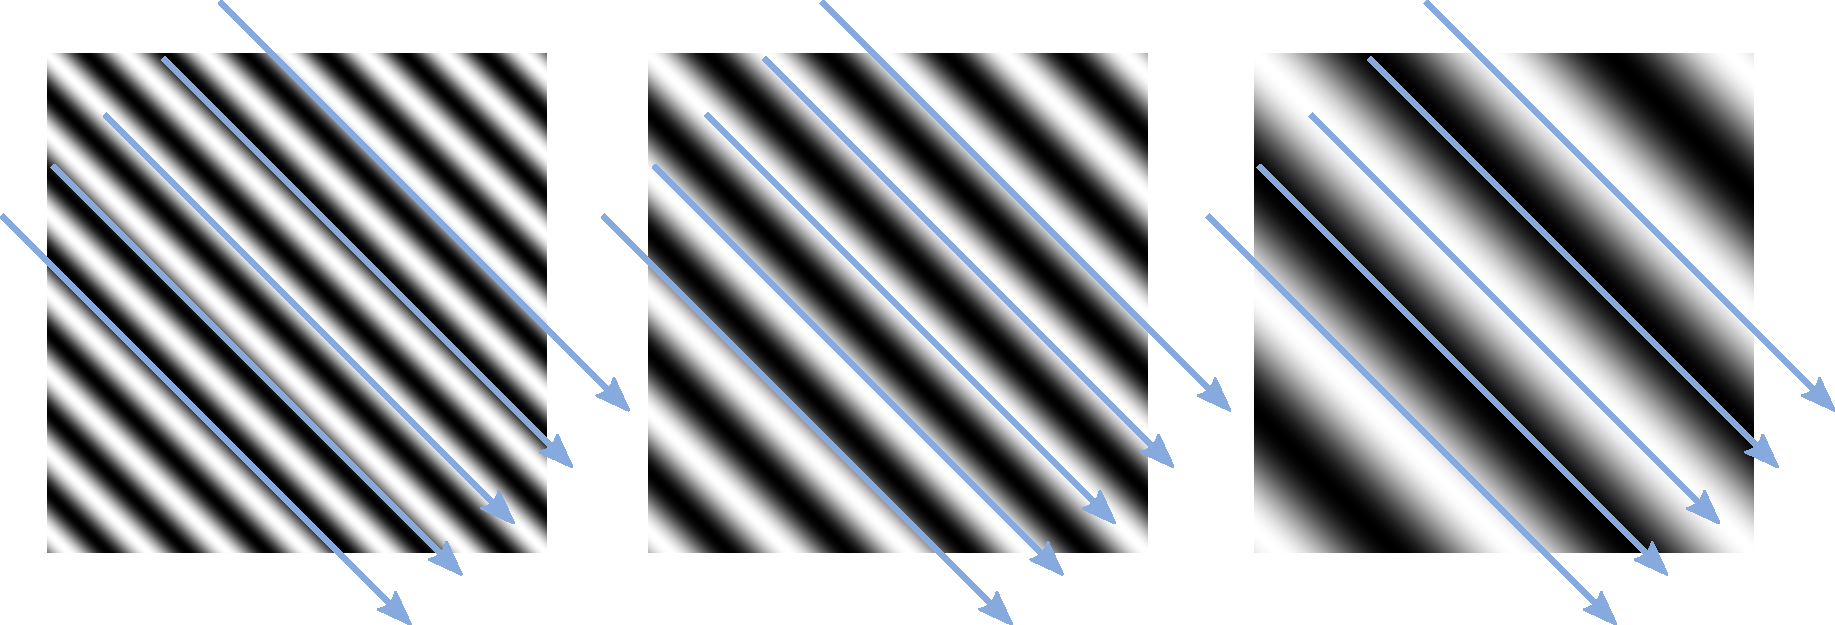
\includegraphics[height=0.6\textheight]{images/ProjetionAndFourierTransform}
\end{frame}

\subtitle{Computed Tomography --- Part 2}
\frame[plain,c]{\titlepage}

\section{Image Reconstruction}

\begin{frame}
	\frametitle{How do we get volumetric images?}

	\begin{itemize}
		\item We'll see 2 methods for 2-D reconstruction from parallel projections
		\item Conventional CT:\ 3-D volume is obtained by acquiring multiple axial slices
		\item Slices at different positions are stacked:

	\end{itemize}

	\begin{figure}[tbp]
		\centering
		\includegraphics[width=0.85\linewidth]{images/reco_1}%
		%\caption{In conventional CT, a 3-D image of the body is formed by acquiring, reconstructing and subsequently stacking 2-D image slices in axial direction. For each slice, all projection rays lie in a plane, which is why we only deal with bivariate functions $f(x,y)$. However, be aware that there are other geometries where this assumption is no longer valid (\cf~\secRef{sub:ct_geom}).}
		\label{fig:ct_reco_1}
	\end{figure}

\end{frame}

\subsection{Analytic Reconstruction}
\label{sub:ct_analytic}

\begin{frame}[c]{Analytic Reconstruction}

	Using the Fourier Slice Theorem, we derive an analytic reconstruction method:

	\hspace{0.8cm}
	\begin{itemize}
		\setlength\itemsep{0.8cm}
		\item<2-> Inverse Fourier transform of $F(u,v)$:
		      %
		      \begin{equation}
			      \tikz[baseline]{\node[fill=blue!20,anchor=base, rounded corners] (f1) {$f(x,y)$};}
			      = \int_{-\infty}^{+\infty}\int_{-\infty}^{+\infty}
			      \tikz[baseline]{\node[fill=red!20,anchor=base, rounded corners] (F1) {$F(u,v)$};}
			      e^{2\pi i(ux+vy)} \ \textnormal du \textnormal dv
		      \end{equation}

		\item<5-> Rewrite in polar coordinates $F_{\textnormal{polar}}(\omega, \theta)$ by substituting $u = \omega \cos \theta$ and $v = \omega \sin \theta$

		\item<6-> Requires a ``correction'' factor computed from the Jacobian $\boldsymbol J$:
		      \begin{eqnarray}
			      |\det\boldsymbol J| &=&
			      \left|\det\begin{pmatrix}
				      \frac{\textnormal du}{\textnormal d\omega} & \frac{\textnormal du}{\textnormal d\theta}  \\[0.3em]
				      \frac{\textnormal dv}{\textnormal d\omega} & \frac{\textnormal dv}{\textnormal d \theta}
			      \end{pmatrix}\right| =
			      \left|\det\begin{pmatrix}
				      \cos(\theta) & -\omega \sin(\theta) \\[0.3em]
				      \sin(\theta) & \omega \cos(\theta)
			      \end{pmatrix}\right| =\\[0.75em]
			      &=&|\omega \cos^2(\theta) + \omega \sin^2(\theta)| = |\omega|
		      \end{eqnarray}

		      %\item<6-> Perform change in variables:

		      %\begin{equation}
		      %\tikz[baseline]{\node[fill=blue!20,anchor=base, rounded corners] (f2) {$f(x,y)$};}%
		      %= \int_0^\pi \int_{-\infty}^{+\infty}
		      %\tikz[baseline]{\node[fill=red!20,anchor=base, rounded corners] (F2) {$F_{\textnormal{polar}}(\omega, \theta)$};}
		      %\alt<6>{%
		      %\tikz[baseline]{\node[fill=yellow!30,anchor=base, rounded corners] (F2) {$|\omega|$};}
		      %}{%
		      %\tikz[baseline]{\node[anchor=base, rounded corners] (F2) {$|\omega|$};}
		      %}%
		      %e^{2 \pi i \omega (x \cos \theta + y \sin \theta)} \ \textnormal d\omega \textnormal d\theta.
		      %\end{equation}
	\end{itemize}
	\visible<3-4>{\begin{tikzpicture}[remember picture,overlay]
			\node[xshift=-6cm,yshift=-4.9cm, fill=red!20,anchor=base, rounded corners] at (current page.north east) (a){Fourier transform of slice};
			\node[xshift=-6.9cm,yshift=-3.9cm, fill=red!20, coordinate] at (current page.north east) (b){};
			\path[draw=faublue,->, line width=0.4mm] (a) -- (b) ;
			\visible<4>{
				\node[xshift=-11cm,yshift=-4.9cm, fill=blue!20,anchor=base, rounded corners] at (current page.north east) (a){Reconstructed slice};
				\node[xshift=-10.3cm,yshift=-3.9cm, fill=blue!20, coordinate] at (current page.north east) (b){};
				\path[draw=faublue,->, line width=0.4mm] (a) -- (b) ;}
		\end{tikzpicture}}
	%\visible<6>{\begin{tikzpicture}[remember picture,overlay]
	%\node[xshift=-5.5cm,yshift=-8.1cm, fill=yellow!30,anchor=base, rounded corners] at (current page.north east) (a){Factor from transform to polar coordinates};
	%\node[xshift=-6.8cm,yshift=-7.0cm, fill=blue!20, coordinate] at (current page.north east) (b){};
	%\path[draw=faublue,->, line width=0.4mm] (a) -- (b);
	%\end{tikzpicture}}

\end{frame}

\begin{frame}[c]{Analytic Reconstruction}

	Using the Fourier Slice Theorem, we derive an analytic reconstruction method:

	\hspace{0.8cm}
	\begin{itemize}
		\setlength\itemsep{0.8cm}

		\item<1-> Requires a ``correction'' factor computed from the Jacobian $\boldsymbol J$:
		      \begin{eqnarray}
			      |\det\boldsymbol J| &=&
			      \left|\det\begin{pmatrix}
				      \frac{\textnormal du}{\textnormal d\omega} & \frac{\textnormal du}{\textnormal d\theta}  \\[0.3em]
				      \frac{\textnormal dv}{\textnormal d\omega} & \frac{\textnormal dv}{\textnormal d \theta}
			      \end{pmatrix}\right| =
			      \left|\det\begin{pmatrix}
				      \cos(\theta) & -\omega \sin(\theta) \\[0.3em]
				      \sin(\theta) & \omega \cos(\theta)
			      \end{pmatrix}\right| =\\[0.75em]
			      &=&|\omega \cos^2(\theta) + \omega \sin^2(\theta)| = |\omega|
		      \end{eqnarray}

		\item<2-> Perform change in variables:

		      \begin{equation}
			      \tikz[baseline]{\node[fill=blue!20,anchor=base, rounded corners] (f2) {$f(x,y)$};}%
			      = \int_0^\pi \int_{-\infty}^{+\infty}
			      \tikz[baseline]{\node[fill=red!20,anchor=base, rounded corners] (F2) {$F_{\textnormal{polar}}(\omega, \theta)$};}
			      \tikz[baseline]{\node[fill=yellow!30,anchor=base, rounded corners] (F2) {$|\omega|$};}
			      e^{2 \pi i \omega (x \cos \theta + y \sin \theta)} \ \textnormal d\omega \textnormal d\theta.
		      \end{equation}
	\end{itemize}
	%\visible<3-4>{\begin{tikzpicture}[remember picture,overlay]
	%\node[xshift=-6cm,yshift=-4.9cm, fill=red!20,anchor=base, rounded corners] at (current page.north east) (a){Fourier transform of slice};
	%\node[xshift=-6.9cm,yshift=-3.9cm, fill=red!20, coordinate] at (current page.north east) (b){};
	%\path[draw=faublue,->, line width=0.4mm] (a) -- (b) ;
	%\visible<4>{
	%\node[xshift=-11cm,yshift=-4.9cm, fill=blue!20,anchor=base, rounded corners] at (current page.north east) (a){Reconstructed slice};
	%\node[xshift=-10.3cm,yshift=-3.9cm, fill=blue!20, coordinate] at (current page.north east) (b){};
	%\path[draw=faublue,->, line width=0.4mm] (a) -- (b) ;}
	%\end{tikzpicture}}
	%\visible<6>{\begin{tikzpicture}[remember picture,overlay]
	%\node[xshift=-5.5cm,yshift=-8.1cm, fill=yellow!30,anchor=base, rounded corners] at (current page.north east) (a){Factor from transform to polar coordinates};
	%\node[xshift=-6.8cm,yshift=-7.0cm, fill=blue!20, coordinate] at (current page.north east) (b){};
	%\path[draw=faublue,->, line width=0.4mm] (a) -- (b);
	%\end{tikzpicture}}

\end{frame}

\begin{frame}[c]{Analytic Reconstruction}

	\only<1-2>{\begin{itemize}
			\setlength\itemsep{0.6cm}
			      %\begin{equation}
			      %f(x,y) = \int_0^\pi \int_{-\infty}^{+\infty}  |\omega| e^{2 \pi i \omega (x \cos \theta + y \sin \theta)} \ \textnormal d\omega \textnormal d\theta.
			      %\end{equation}
			\item From Fourier Slice Theorem, we know $%
				      \tikz[baseline]{\node[fill=red!20,anchor=base, rounded corners] (f2) {$F_{\textnormal{polar}}(\omega, \theta)$};}%
				      =
				      \tikz[baseline]{\node[fill=green!20,anchor=base, rounded corners] (f2) {${P(\omega, \theta)}$};}%
			      $:

			      \begin{equation}
				      \tikz[baseline]{\node[fill=blue!20,anchor=base, rounded corners] (f2) {$f(x,y)$};}%
				      = \int_0^\pi \int_{-\infty}^{+\infty}
				      \alt<1>{%
					      \tikz[baseline]{\node[fill=red!20,anchor=base, rounded corners, text width=2cm, align=center] (f2) {$F_{\textnormal{polar}}(\omega, \theta)$};}%
				      }%
				      {
					      %
					      \tikz[baseline]{\node[fill=green!20,anchor=base, rounded corners, text width=2cm, align=center] (f2) {${P(\omega, \theta)}$};}%
				      }%
				      |\omega| e^{2 \pi i \omega (x \cos \theta + y \sin \theta)} \ \textnormal d\omega \textnormal d\theta.
			      \end{equation}

			\item Replace $x \cos \theta + y \sin \theta$ with $s$:

			      \begin{equation}
				      \label{eqn:ct_analytic_1}
				      \tikz[baseline]{\node[fill=blue!20,anchor=base, rounded corners] (f2) {$f(x,y)$};}%
				      = \int_0^\pi \int_{-\infty}^{+\infty}%
				      \tikz[baseline]{\node[fill=green!20,anchor=base, rounded corners] (f2) {${P(\omega, \theta)}$};}%
				      |\omega| e^{2 \pi i \omega s} \ \textnormal d\omega \textnormal d\theta
			      \end{equation}

			      %\item [$\Rightarrow$] Filtered Backprojection algorithm
		\end{itemize}}

\end{frame}

\begin{frame}[t]{Filtered Backprojection Algorithm}

	\begin{itemize}
		\setlength\itemsep{0.5cm}

		\item Product in Fourier space $\leftrightarrow$ convolution in spatial domain
		      \begin{equation}
			      \label{eqn:ct_analytic_4}
			      \tikz[baseline]{\node[fill=blue!20,anchor=base, rounded corners] (f2) {$f(x,y)$};}%
			      = \int_0^\pi \int_{-\infty}^{+\infty}
			      \tikz[baseline]{\node[fill=green!20,anchor=base, rounded corners] (f2) {${P(\omega, \theta)}$};}%
			      \tikz[baseline]{\node[fill=yellow!30,anchor=base, rounded corners] (f2) {$|\omega|$};}%
			      e^{2 \pi i \omega s} \ \textnormal d\omega \textnormal d\theta
		      \end{equation}
		\item With $h(s)$ inverse Fourier transform of $|\omega|$

		      \begin{equation}
			      \label{eqn:ct_analytic_5}
			      \tikz[baseline]{\node[fill=blue!20,anchor=base, rounded corners] (f2) {$f(x,y)$};}%
			      = \int_{0}^\pi
			      \tikz[baseline]{\node[fill=green!20,anchor=base, rounded corners] (f2) {${p(s, \theta)}$};}%
			      *
			      \tikz[baseline]{\node[fill=yellow!30,anchor=base, rounded corners] (f2) {$h(s)$};}%
			      |_{s=x \cos \theta + y \sin \theta} \ \textnormal d\theta
		      \end{equation}

		\item Amounts to back-projection of $p_\theta(s)$ convolved with filter kernel $h(s)$
		      %\item[$\Rightarrow$] ``Filtered Back-Projection'' (FBP) algorithm

		      %\item NB: Unfiltered BP $\leftrightarrow$ adding $P_\theta(\omega)$ to $F(u, v)$ (dual of Radon transform)
	\end{itemize}
	\visible<2>{\begin{tikzpicture}[overlay]
			\node[xshift=-6cm,yshift=-6.2cm, fill=yellow!30,anchor=base, rounded corners] at (current page.north east) (a){Filter};
			\node[xshift=-6.8cm,yshift=-5.6cm, fill=red!20, coordinate] at (current page.north east) (b){};
			\node[xshift=-7.3cm,yshift=-6.8cm, fill=red!20, coordinate] at (current page.north east) (c){};
			\path[draw=faublue,->, line width=0.4mm] (a) -- (b);%
			\path[draw=faublue,->, line width=0.4mm] (a) -- (c);%
		\end{tikzpicture}
	}
\end{frame}

\begin{frame}
	\frametitle{Filter}

	\begin{figure}[tbp]
		\centering
		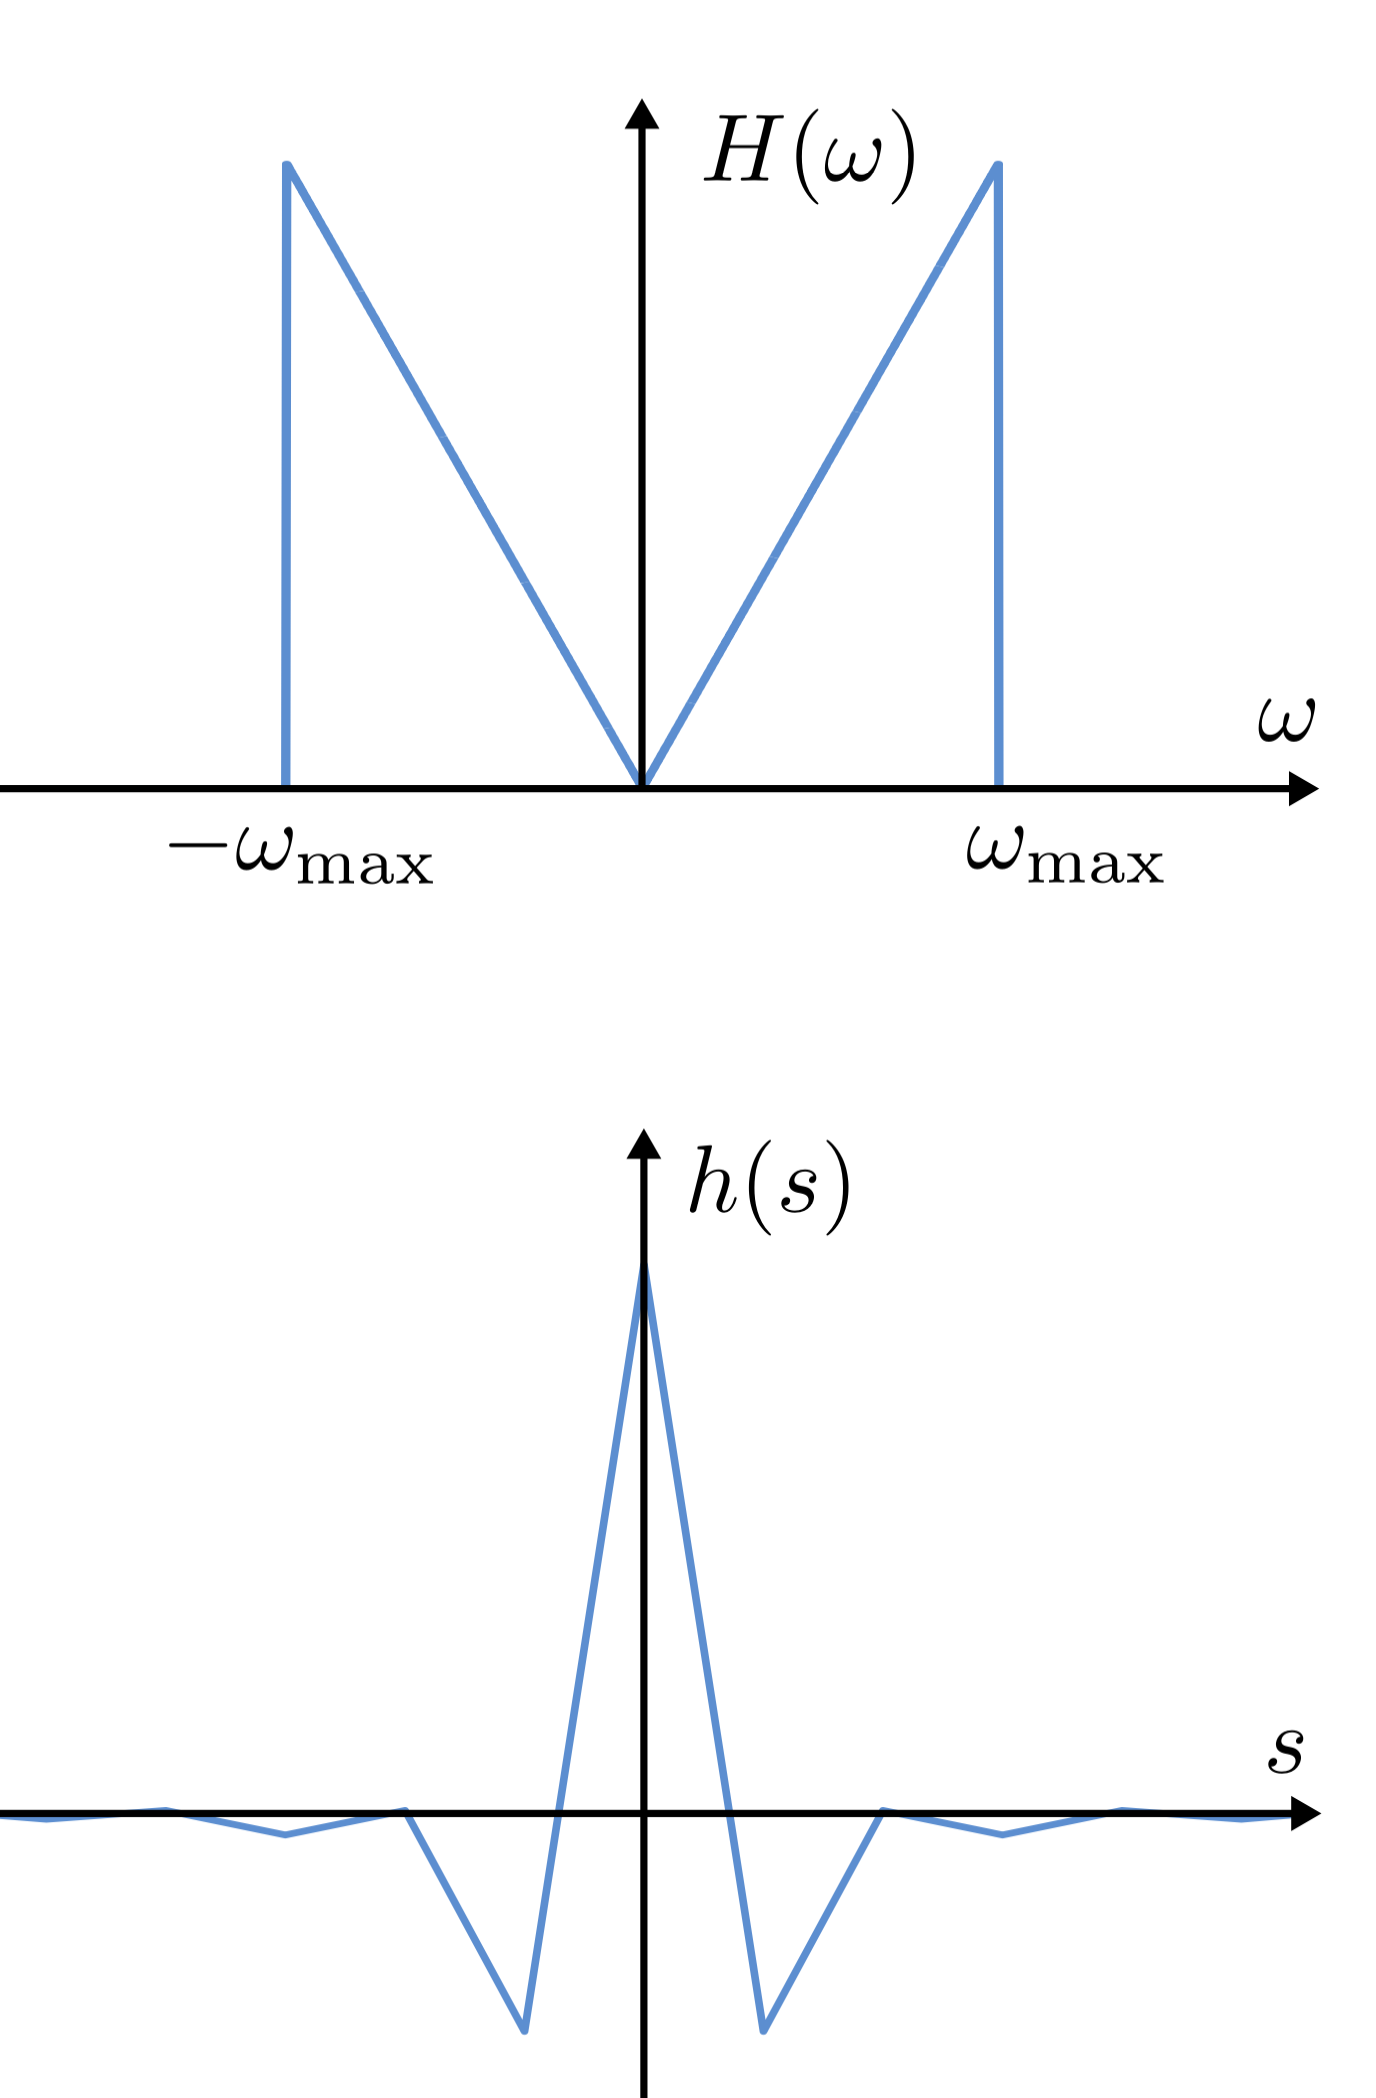
\includegraphics[width=0.25\linewidth]{images/analytic_2_ram_lak.png}
		\caption{The responses in frequency domain as well as the discretized spatial domain kernels of the Ram-Lak filter.}
	\end{figure}
\end{frame}

\begin{frame}
	\frametitle{Filters}

	\begin{itemize}
		\setlength\itemsep{0.3cm}
		\item $h(s)$ is called ``ramp filter'' due to shape of $|\omega|$
		\item Polar coordinates lead to oversampling of Fourier space center
		\item Ramp filter ``fixes'' this by appropriate weighting of frequencies

		\item Fourier domain
		      \begin{equation}
			      \tikz[baseline]{\node[fill=blue!20,anchor=base, rounded corners] (f2) {$f(x,y)$};}%
			      = \int_0^\pi \int_{-\infty}^{+\infty}
			      \tikz[baseline]{\node[fill=green!20,anchor=base, rounded corners] (f2) {${P(\omega, \theta)}$};}%
			      \tikz[baseline]{\node[fill=yellow!30,anchor=base, rounded corners] (f2) {$|\omega|$};}%
			      e^{2 \pi i \omega s} \ \textnormal d\omega \textnormal d\theta
		      \end{equation}
		\item Spatial domain
		      \begin{equation}
			      \label{eqn:ct_analytic_2}
			      \tikz[baseline]{\node[fill=blue!20,anchor=base, rounded corners] (f2) {$f(x,y)$};}%
			      = \int_{0}^\pi
			      \tikz[baseline]{\node[fill=green!20,anchor=base, rounded corners] (f2) {${p(s, \theta)}$};}%
			      *
			      \tikz[baseline]{\node[fill=yellow!30,anchor=base, rounded corners] (f2) {$h(s)$};}%
			      |_{s=x \cos \theta + y \sin \theta} \ \textnormal d\theta
		      \end{equation}
	\end{itemize}

\end{frame}

\begin{frame}
	\frametitle{Importance of Ramp Filtering}

	\begin{figure}[tb]
		\centering
		\begin{minipage}{.4\linewidth}
			\centering
			\includegraphics[height=0.65\textheight]{images/analytic_1}
			\captionof{figure}{Sampling in polar coordinates causes the density of samples to increase with proximity to the origin, whereas the more distant areas are under-represented.}
			\label{fig:ct_analytic_1}
		\end{minipage}%
		\hspace{1.3cm}
		\begin{minipage}{.4\linewidth}
			\centering
			\includegraphics[height=0.65\textheight]{images/analytic_3}
			\captionof{figure}{The back-projection $b_\theta(x,y)$ of a single projection $p_\theta(s)$ hardly gives us an idea of the original function $f(x,y)$. However, we can reconstruct it by back-projecting a sufficient set of appropriately filtered projections.}
			\label{fig:ct_analytic_3}
		\end{minipage}
	\end{figure}

\end{frame}

\begin{frame}[c]{Filters}

	\begin{itemize}
		\setlength\itemsep{0.5cm}
		\item Sampling theorem: detector spacing of $\Delta s$
		      \begin{itemize}
			      \item[$\Rightarrow$] largest frequency detectable in $p_\theta(s)$ is $\omega_{\textnormal{max}} = \frac{1}{2\Delta s}$
		      \end{itemize}
		\item Additionally, noise is amplified by ramp filter $|\omega|$
		      \begin{itemize}
			      \item[$\Rightarrow$] High frequencies should be limited
		      \end{itemize}
		\item Generalize by replacing $|\omega|$ with an arbitrary filter $H(\omega)$:
		      \begin{equation}
			      \tilde{p}_{\theta}(s) = \int_{-\infty}^{+\infty} P(\omega, \theta) H(\omega) e^{2 \pi i \omega s} \ \textnormal d\omega,
		      \end{equation}

	\end{itemize}

\end{frame}

\begin{frame}
	\frametitle{Filters}

	\begin{itemize}
		\item In practice: ramp-like filters with various characteristics
		\item Trade-off between smoothness and spatial resolution
		\item Well known filter by Ramachandran and Lakshminarayanan (``Ram-Lak''):

		      \begin{equation}
			      h(s) = \frac{\operatorname{sinc}\left(\frac{\pi s}{\Delta s}\right)}{2 (\Delta s)^2} - \frac{\operatorname{sinc}^2\left(\frac{\pi s}{2\Delta s}\right)}{4 (\Delta s)^2},
		      \end{equation}

		\item Corresponds to $|\omega|$ cut off at $\omega_\text{max}$

		\item Apply windowing function in frequency domain to suppress noise
		\item Often used windowing function (leads to Shepp-Logan filter):
		      \begin{equation}
			      \left|\operatorname{sinc}\left(\frac{\pi \omega}{2\,\omega_\text{max}}\right)\right|
		      \end{equation}

		\item Filters are discretized for convolution with discrete projections
	\end{itemize}

\end{frame}

\begin{frame}
	\frametitle{Filters}

	\begin{figure}[tbp]
		\centering
		\includegraphics[width=0.5\linewidth]{images/analytic_2}
		\caption{The responses in frequency domain as well as the discretized spatial domain kernels of the Ram-Lak and Shepp-Logan filters.}
	\end{figure}
\end{frame}

\begin{frame}
	\frametitle{Discretization}

	\begin{itemize}
		\item Convolution


		      \begin{equation}
			      \tilde{p}_{\theta}(s) = \int_{-\infty}^{+\infty} p_\theta(s) \cdot h(s - s') \ \textnormal d s'
		      \end{equation}
		      becomes
		      \begin{equation}
			      \tilde{p}_{\theta, s} = \sum_{s'} p_{\theta, s} \cdot h_{s - s'}\ \Delta s.
		      \end{equation}

		
	\end{itemize}

\end{frame}


\begin{frame}
	\frametitle{Discretization}

	\begin{itemize}
		\item Convolution


		      \begin{equation}
			      \tilde{p}_{\theta}(s) = \int_{-\infty}^{+\infty} p_\theta(s) \cdot h(s - s') \ \textnormal d s'
		      \end{equation}
		      becomes
		      \begin{equation}
			      \tilde{p}_{\theta, s} = \sum_{s'} p_{\theta, s} \cdot h_{s - s'}\ \Delta s.
		      \end{equation}

		\item Final backprojection step in \eqref{eqn:ct_analytic_3}:
		      \begin{equation}
			      \label{eqn:ct_analytic_3}
			      f(x, y) = \frac{\pi}{N} \sum_i \tilde{p}_{\theta_i}(s) |_{s=x \cos \theta_i + y \sin \theta_i}
		      \end{equation}

		%\item NB: $\tilde{p}_{\theta_i}(s)$ is interpolated from $\tilde{p}_{\theta_i, s}$
		%\item Rule of thumb: Avoid interpolation in output space, i.\,e.~sample $f$ directly
		%\item This comes naturally with Eq.~\ref{eqn:ct_analytic_3} (voxel-driven BP)

	\begin{figure}[tbp]
		\centering
		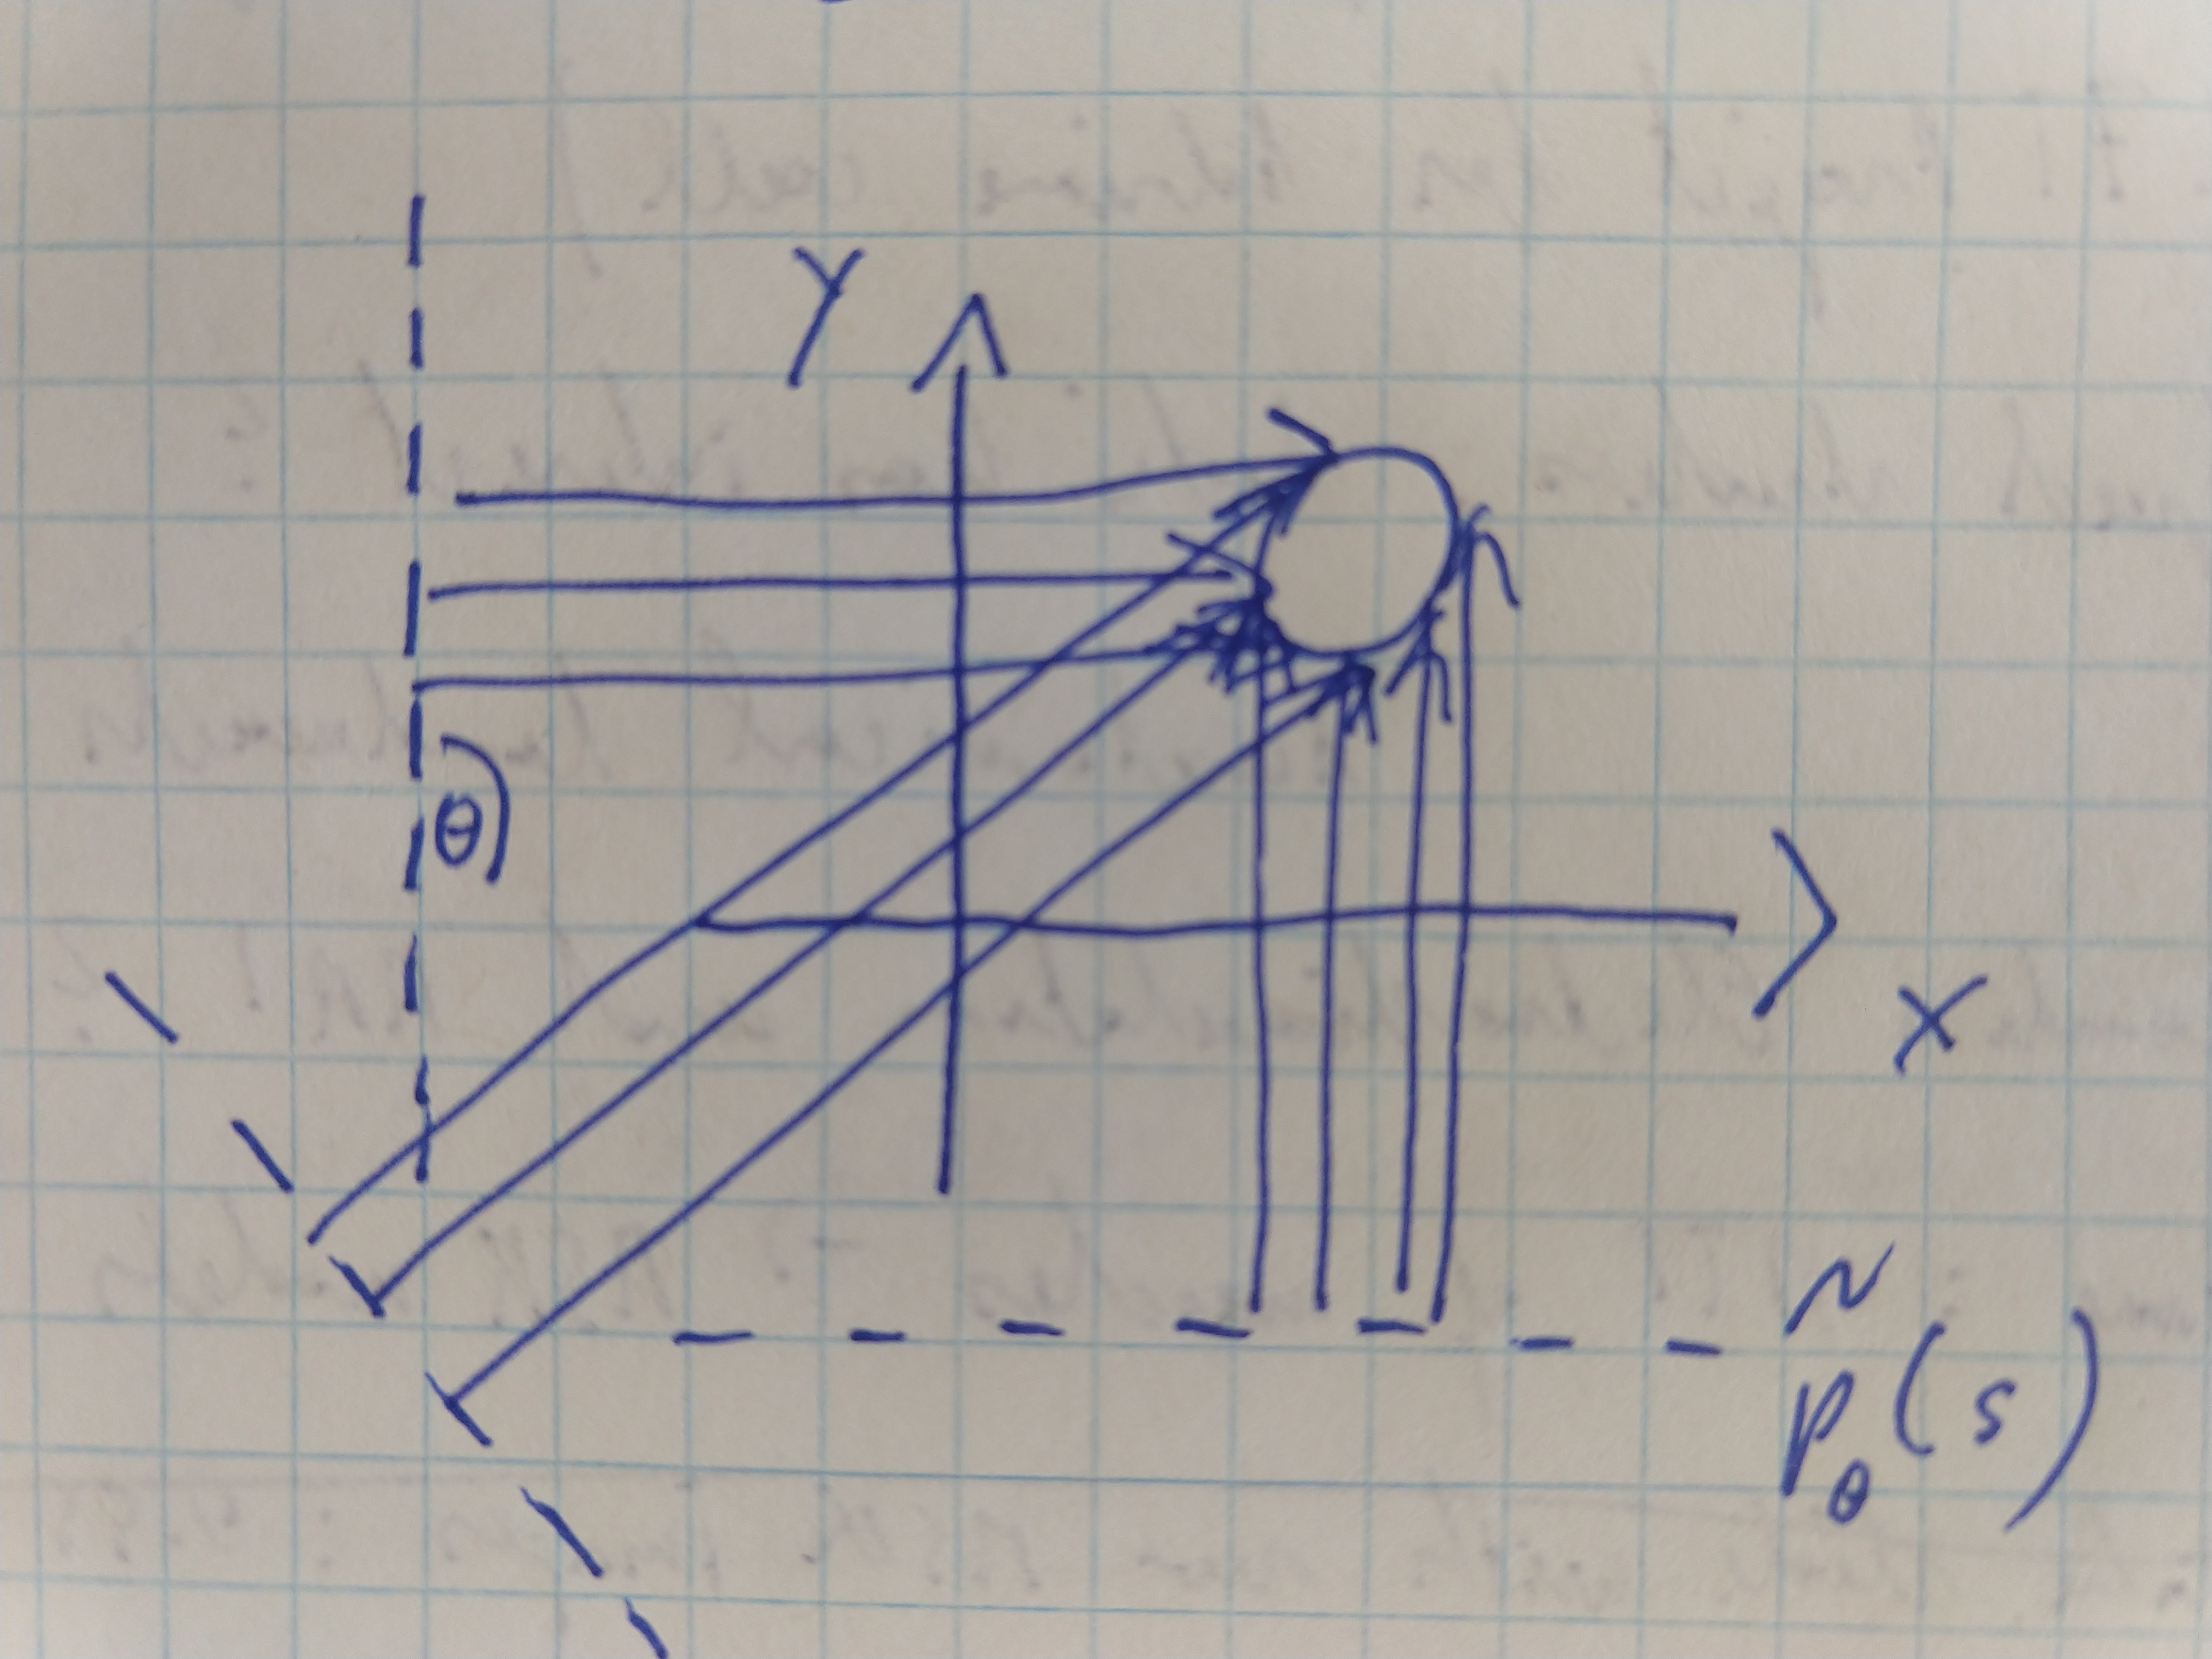
\includegraphics[width=0.15\linewidth]{images/backprojection_sketch}
		%\caption{Todo.}
	\end{figure}
	
	\end{itemize}

\end{frame}

\subsection{Algebraic Reconstruction}
\label{sub:ct_algebraic}

\begin{frame}
	\frametitle{Algebraic Reconstruction}

	\begin{itemize}
		\item Formulate reconstruction problem as a system of linear equations
		\item Sum of pixels each ray passes through should
		      equal measured line integral for that ray
	\end{itemize}

	\begin{figure}[tbp]
		\centering
		\includegraphics[height=0.6\textheight]{images/algebraic_1}
		\caption{Example for an image grid and some projection rays.}
		\label{fig:ct_algebraic_1}
	\end{figure}
\end{frame}

\begin{frame}
	\frametitle{Algebraic Reconstruction}

	\begin{itemize}
		\item Formulate reconstruction problem as a system of linear equations
		\item Sum of pixels each ray passes through should equal measured line integral for that ray
		\item Example: $p_3 = x_2 \alpha_1 + x_3 \alpha_2 + x_6 \alpha_3$     
	\end{itemize}

	\begin{figure}[tbp]
		\centering
		\includegraphics[height=0.6\textheight]{images/algebraic_1}
		\caption{Example for an image grid and some projection rays.}
	\end{figure}
\end{frame}

\begin{frame}
	\frametitle{Algebraic Reconstruction}

	\begin{equation}
		\label{eqn:ct_algebraic_1}
		\mat{A}\vec{x} = \vec{p}
	\end{equation}

	\begin{eqnarray*}
		\vec{x} &= (x_1, x_2,...,x_N)^\top &\quad \text{are the unknown pixels,} \\
		\vec{p} &= (p_1, p_2,...,p_N)^\top &\quad \text{are the measured values.}
	\end{eqnarray*}

	\begin{itemize}
		\item Each element $a_{ij}$ of system matrix $\mat{A}$ holds contribution of a pixel to a ray
		\item Choices in modeling $a_{ij}$:
		      \begin{itemize}
			      \item Binary value ($1$ if ray touches the pixel, $0$ otherwise)
			      \item Length of intersection
			      \item Area of intersection (rays with non-zero thickness)
		      \end{itemize}
		\item $\mat{A}^{-1} \vec{p}$ corresponds to the inverse Radon transform
	\end{itemize}
\end{frame}

\begin{frame}[c]{Solving the System}

	\bluefat{Simple matrix inversion not feasible:}

	\begin{itemize}
		\setlength\itemsep{0.3cm}
		\item Problems are large, ill-conditioned and over-determined
		      \begin{itemize}
			      \item[$\Rightarrow$] Try iterative approaches instead
		      \end{itemize}
	\end{itemize}
	\vspace{1cm}

	\bluefat{Algebraic Reconstruction Technique (ART):}
	\begin{itemize}
		\item Kaczmarz method
		\item Basic idea:
		      \begin{itemize}
			      \item Each equation defines a line (2-D) / hyper plane (higher dim.) in solution space
			      \item All points on the hyper plane fulfill the equation
			            \begin{itemize}
				            \item[$\Rightarrow$] Solution is in the point of intersection
			            \end{itemize}
			      \item To get there, repeatedly project orthogonally onto different equations
		      \end{itemize}

	\end{itemize}

\end{frame}

%\begin{frame}
%	\frametitle{Kaczmarz Method}
%
%	\begin{figure}[tbp]
%		\centering
%		\includegraphics[height=0.8\textheight]{images/algebraic_2}
%		\caption{Kaczmarz iterations in 2-D space.}
%		\label{fig:ct_algebraic_2}
%	\end{figure}
%
%\end{frame}
%
%\begin{frame}
%	\frametitle{Geometry Basics}
%
%	\begin{itemize}
%		\item 2-D case: point $\vec x$, line $\vec n^\top\vec c = d$ ($\vec c$ is a point on the line)
%		\item Orthogonal projection $\vec{x'}$ of $\vec{x}$ is along normal $\vec n$:
%
%		      \begin{equation}
%			      \label{eqn:ct_algebraic_2}
%			      \vec{x'} = \vec{x} + \lambda \vec{n}
%		      \end{equation}
%
%		\item $\vec{x'}$ must be on the line: $\vec{n}^\top\vec{x'} = d$
%
%		\item Plug this into Eq.~\ref{eqn:ct_algebraic_2}:
%
%		      \begin{eqnarray}
%			      \vec{n}^\top(\vec{x} + \lambda \vec{n}) = d\\
%			      \lambda = \frac{d-\vec{n}^\top\vec{x}}{\vec{n}^\top\vec{n}}
%		      \end{eqnarray}
%
%		\item Substitute $\lambda$ in Eq.~\ref{eqn:ct_algebraic_2}:
%		      \begin{equation}
%			      \vec{x'} = \vec{x} + \frac{d - \vec{n}^\top \vec{x}}{\vec{n}^\top\vec{n}}\vec{n}
%		      \end{equation}
%
%	\end{itemize}
%
%\end{frame}
%
%\begin{frame}
%
%	\frametitle{Kaczmarz Update Formula}
%
%	\begin{itemize}
%
%		\item Reminder: We want to iteratively solve $\mat A \vec x = \vec p$
%
%		\item Update step (for each \emph{row} $a_i$ of $\mat A$):
%
%		      \begin{equation}
%			      \vec{x}^{k+1} = \vec{x}^k + \frac{p_i - \vec{a}_i\vec{x}^k}{\vec{a}_i\vec{a}^\top_i}\vec{a}^\top_i,
%		      \end{equation}
%
%		\item This is just our projection formula with different symbols! Compare:
%		      \begin{equation}
%			      \vec{x'} = \vec{x} + \frac{d - \vec{n}^\top \vec{x}}{\vec{n}^\top\vec{n}}\vec{n}
%		      \end{equation}
%
%	\end{itemize}
%
%\end{frame}
%
%\begin{frame}[t]{Notes on Kaczmarz}
%
%	\begin{itemize}
%		\setlength\itemsep{0.3cm}
%		\item Tanabe (1971): If a unique solution exists, Kaczmarz converges to it
%		\item But: No unique solution exists in over-determined and noisy systems
%		      \begin{itemize}
%			      \item[$\Rightarrow$] oscillation around the ideal solution
%		      \end{itemize}
%		\item Rate of convergence dependant on angles between lines
%		\item Orthogonalization methods can improve convergence
%		      \begin{itemize}
%			      \item Computationally demanding
%			      \item Amplifies noise
%		      \end{itemize}
%	\end{itemize}
%
%\end{frame}
%
%\begin{frame}
%	\frametitle{Extensions to ART}
%
%	\begin{itemize}
%		\item ``Ordered subsets'': Select sequence of projections in a clever way
%		\item Simultaneous ART (SART): Do multiple updates at the same time and use the centroid:
%
%		      \begin{equation}
%			      \vec{x}^{k+1} = \vec{x}^k + \lambda_k \sum_{i} u_{k,i} \frac{p_i - \vec{a}_i\vec{x}^k}{\vec{a}_i\vec{a}^\top_i}\vec{a}^\top_i
%		      \end{equation}
%		      with
%		      \begin{equation}
%			      \sum_{i}u_{k,i} = 1
%		      \end{equation}
%
%		\item Other optimization approaches: gradient descent, expectation-maximization, regularized reconstruction, \ldots
%	\end{itemize}
%
%\end{frame}

\begin{frame}
	\frametitle{Image Reconstruction}

	\begin{itemize}
		\setlength\itemsep{0.3cm}
		\item Beer's law: Convert X-ray projections $\rightarrow$ line integrals images
		\item We can apply Radon's ideas for X-ray CT reconstruction!
		\item Slice of our object corresponds to $f(x,y)$
		\item More precisely: function values are the linear attenuation coefficients
		\item Typically linearly transformed to the Hounsfield scale:
		      %%
		      \begin{equation}
			      \mu^* = \left( \frac{\mu}{\mu_\text{Water}} - 1 \right) \cdot 1000,
		      \end{equation}
		      %%
	\end{itemize}

\end{frame}

\begin{frame}[c]{Hounsfield Units}

	\begin{table}[tbp]
		\centering
		\begin{tabular}{ll}
			\toprule
			Material / Tissue & Hounsfield Units \\
			\midrule
			Air               & $-1000$          \\
			Lung              & $-600$ to $-400$ \\
			Fat               & $-100$ to $-60$  \\
			Water             & $0$              \\
			Muscle            & $10$ to $40$     \\
			Blood             & $30$ to $45$     \\
			Soft Tissue       & $40$ to $80$     \\
			Bone              & $400$ to $3000$  \\
			\bottomrule
		\end{tabular}%
		%       \caption{Hounsfield units observed in several materials and tissue classes found in the human body. In general, denser structures exhibit larger Hounsfield values.}
		\label{tab:ct_reco_1}
	\end{table}

\end{frame}


\subsection{Acquisition Geometries}
\label{sub:ct_geom}

\begin{frame}[c,allowframebreaks]{Acquisition Geometries}

	\begin{figure}[tbp]
		\centering
		\begin{subfigure}[t]{0.9\linewidth}
			\centering{}
			\includegraphics[height=0.6\textheight]{images/geom_1}
			\caption{\footnotesize For a parallel beam geometry as introduced in the previous sections (shown on the left), the X-ray source needs to be shifted perpendicularly (dotted line) to the direction of projection, casting pencil beams through the object. If all beams instead emanate from a single position for each angle, we obtain a fan of no longer parallel rays (fan beam geometry; on the right), increasing acquisition efficiency at the cost of a slightly more complicated reconstruction problem. Apart from the flat shape shown here, there also exist curved detectors with an equiangular spacing.}
			\label{fig:ct_geom_1.1}
		\end{subfigure}\\[1cm]
		\begin{subfigure}[t]{0.9\linewidth}
			\centering{}
			\includegraphics[height=0.5\textheight]{images/geom_2}
			\caption{\footnotesize Multiple detector arrays allow for simultaneous acquisition of multiple image slices from one X-ray source position (multi-slice CT; shown on the left). However, in this setup, the beams no longer all lie within the rotation plane. This issue becomes much more important in the case of cone beam CT (shown on the right): Here, the small stack of detector rows gives way to a larger detector matrix, with the beams now forming a cone in 3-D.}
			\label{fig:ct_geom_1.2}
		\end{subfigure}
		%       \caption{Basic acquisition geometries in CT imaging. Blue arrows indicate the trajectory of the X-ray source. The detector is depicted by thick black lines.}
		\label{fig:ct_geom_1}
	\end{figure}

\end{frame}

\begin{frame}
	\frametitle{Scanner Generations}

	\begin{itemize}
		\setlength\itemsep{0.3cm}
		\item CT scanners have been categorized into generations
		\item \textbf{\textcolor{faublue}{1$^\text{st}$ generation}}: Single detector (pencil/parallel beam geometry)
		\item \textbf{\textcolor{faublue}{2$^\text{nd}$ generation}}: Detector arrays (several rays at once)
		\item \textbf{\textcolor{faublue}{3$^\text{rd}$ generation}}: Larger detector arrays (fan beam geometry)
		      \begin{itemize}
			      \item Data can be transformed (``rebinned'') to parallel beam geometry
			      \item Alternatively, explicit fan beam versions of algorithms can be derived
		      \end{itemize}

	\end{itemize}

\end{frame}

\begin{frame}
	\frametitle{2-D Detectors}

	\begin{itemize}
		\setlength\itemsep{0.3cm}
		\item Mult-slice CT: Increased imaging speed (many slices in parallel)
		\item Cone beam CT: 2-D projection images

		      \begin{itemize}
			      \setlength\itemsep{0.1cm}
			      \item Image intensifier or flat panel detector
			      \item Large field of view in a single rotation
			      \item Exact reconstruction only in plane of rotation (incomplete data!)
			      \item Main field of use: Interventional imaging with C-arm devices
		      \end{itemize}

	\end{itemize}

\end{frame}

\begin{frame}
	\frametitle{Interventional C-arm Device}

	\begin{figure}[tbp]
		\centering
		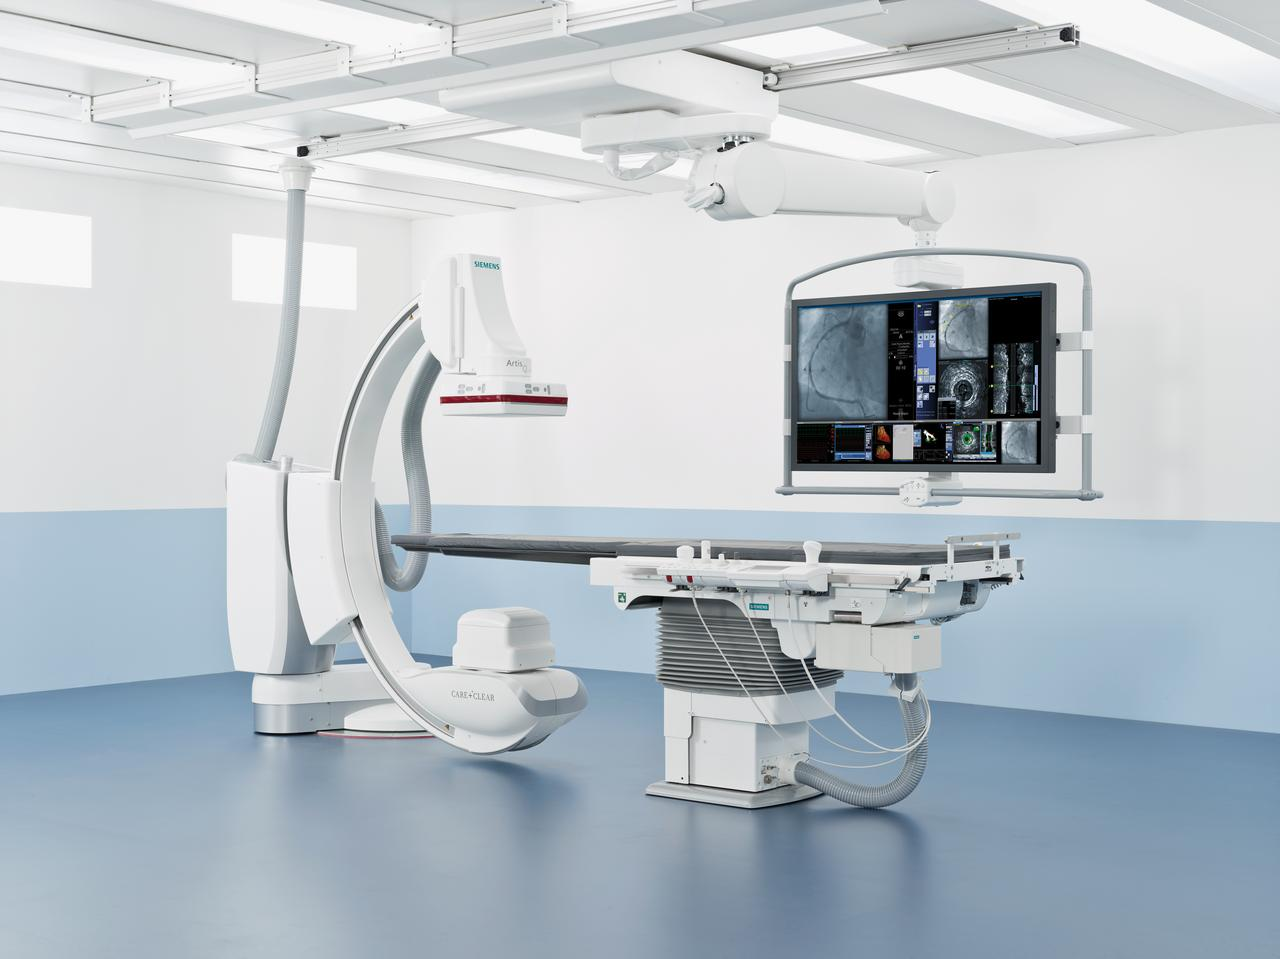
\includegraphics[height=0.8\textheight]{images/c-arm}
		\caption{A C-arm system for interventional X-ray imaging. Image courtesy of Siemens AG.}
		\label{fig:ct_geom_2}
	\end{figure}

\end{frame}

\begin{frame}
	\frametitle{Helical Trajectory: Spiral CT}

	\begin{itemize}
		\setlength\itemsep{0.3cm}
		\item How to image larger parts of the body?
		\item Originally: Rotate, halt, move table; rotate, halt, move table; \ldots
		\item Helical (or spiral) CT: Continuous motion of both gantry and table

		      \hspace{0.1cm}
		      \begin{itemize}
			      \setlength\itemsep{0.2cm}
			      \item Object's point of view: source rotates in $x$-$y$ plane and moves in $z$-direction
			            \begin{itemize}
				            \item[$\Rightarrow$] Trajectory describes a helix
			            \end{itemize}
			      \item Projections for all angles in axial plane can be interpolated

		      \end{itemize}

	\end{itemize}

\end{frame}

\begin{frame}
	\frametitle{Helical Trajectory: Spiral CT}

	\begin{figure}[tbp]
		\centering
		\includegraphics[width=\linewidth]{images/geom_3}
		\caption{In spiral CT, although the X-ray source still conveniently rotates in the $x$-$y$ plane, the trajectory it describes in relation to the imaged object is a helix due to the patient table being slowly moved through the gantry. This enables the acquisition of a large object region while rotating continuously. Projections for an ideal circular trajectory can be interpolated along $z$ from neighboring helical segments.}
		\label{fig:ct_geom_1.3}
	\end{figure}

\end{frame}

\subtitle{Computed Tomography - Part 3}
\frame[plain,c]{\titlepage}

\section{Practical Considerations}
\label{sec:ct_considerations}

%\subsection{From last lecture: Radiation sensitivity of eyes}
%
%\begin{frame}
%    \frametitle{From last lecture: Radiation sensitivity of eyes}
%      \begin{columns}
%		\begin{column}{0.5\textwidth}
%			 \begin{figure}
%        			\centering{}
%       			 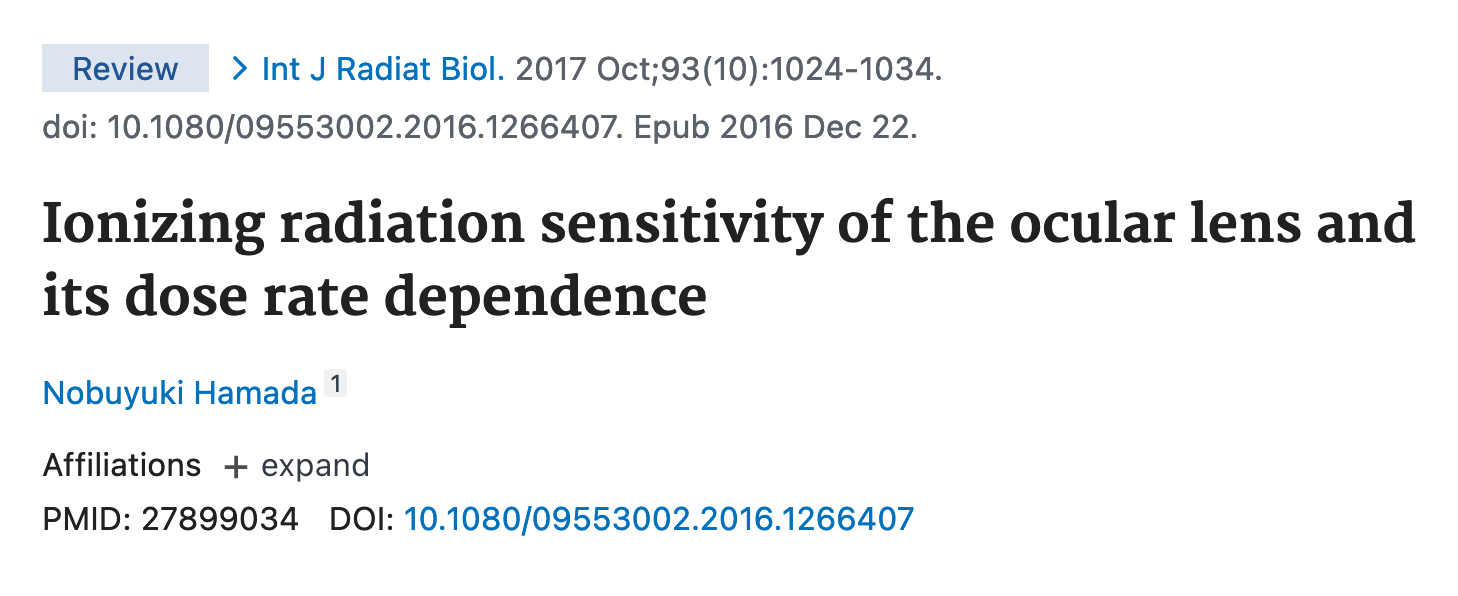
\includegraphics[scale=0.25]{images/hamada_2017_eye_sensitivity_radiation.png}
%    			\end{figure}
%		\end{column}
%			\begin{column}{0.5\textwidth}
%			 \begin{figure}
%        			\centering{}
%       			 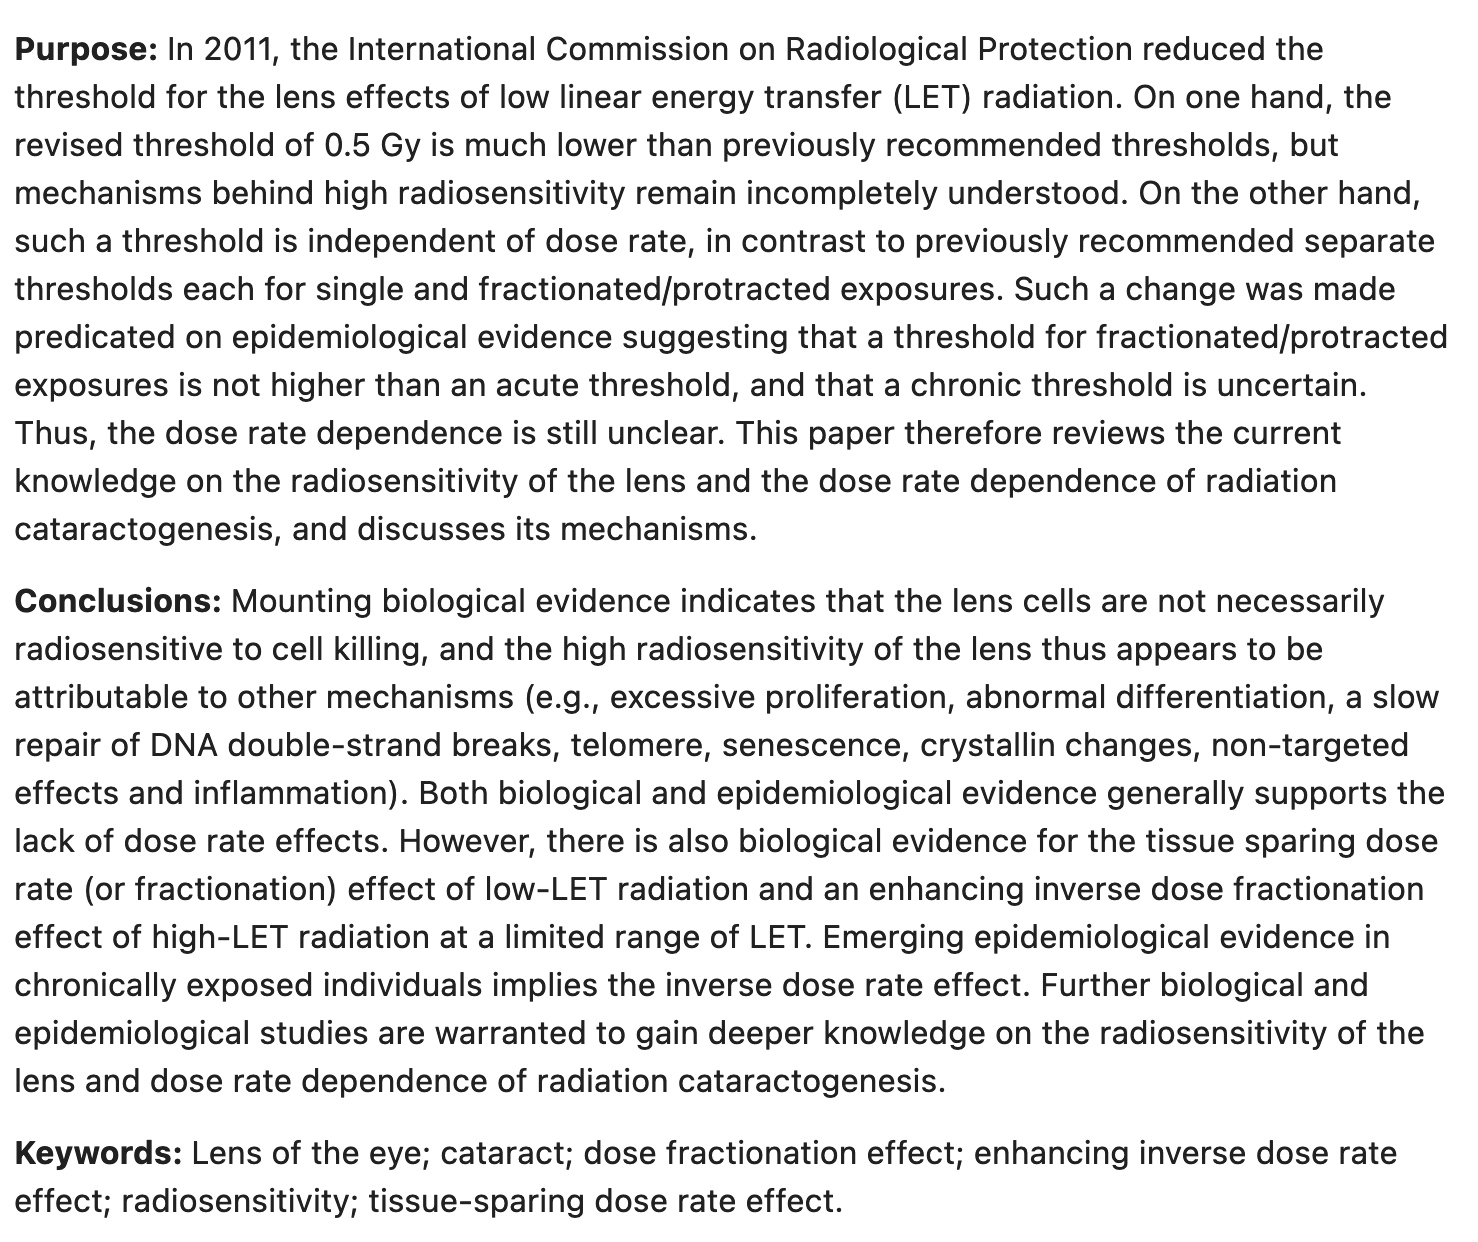
\includegraphics[scale=0.25]{images/hamada_2017_abstract.png}
%    			\end{figure}
%		\end{column}
%	\end{columns}
%\end{frame}

%\begin{frame}
    %\frametitle{Radiation sensitivity of eyes}

	%		 \begin{figure}
        	%		\centering{}
      % 			 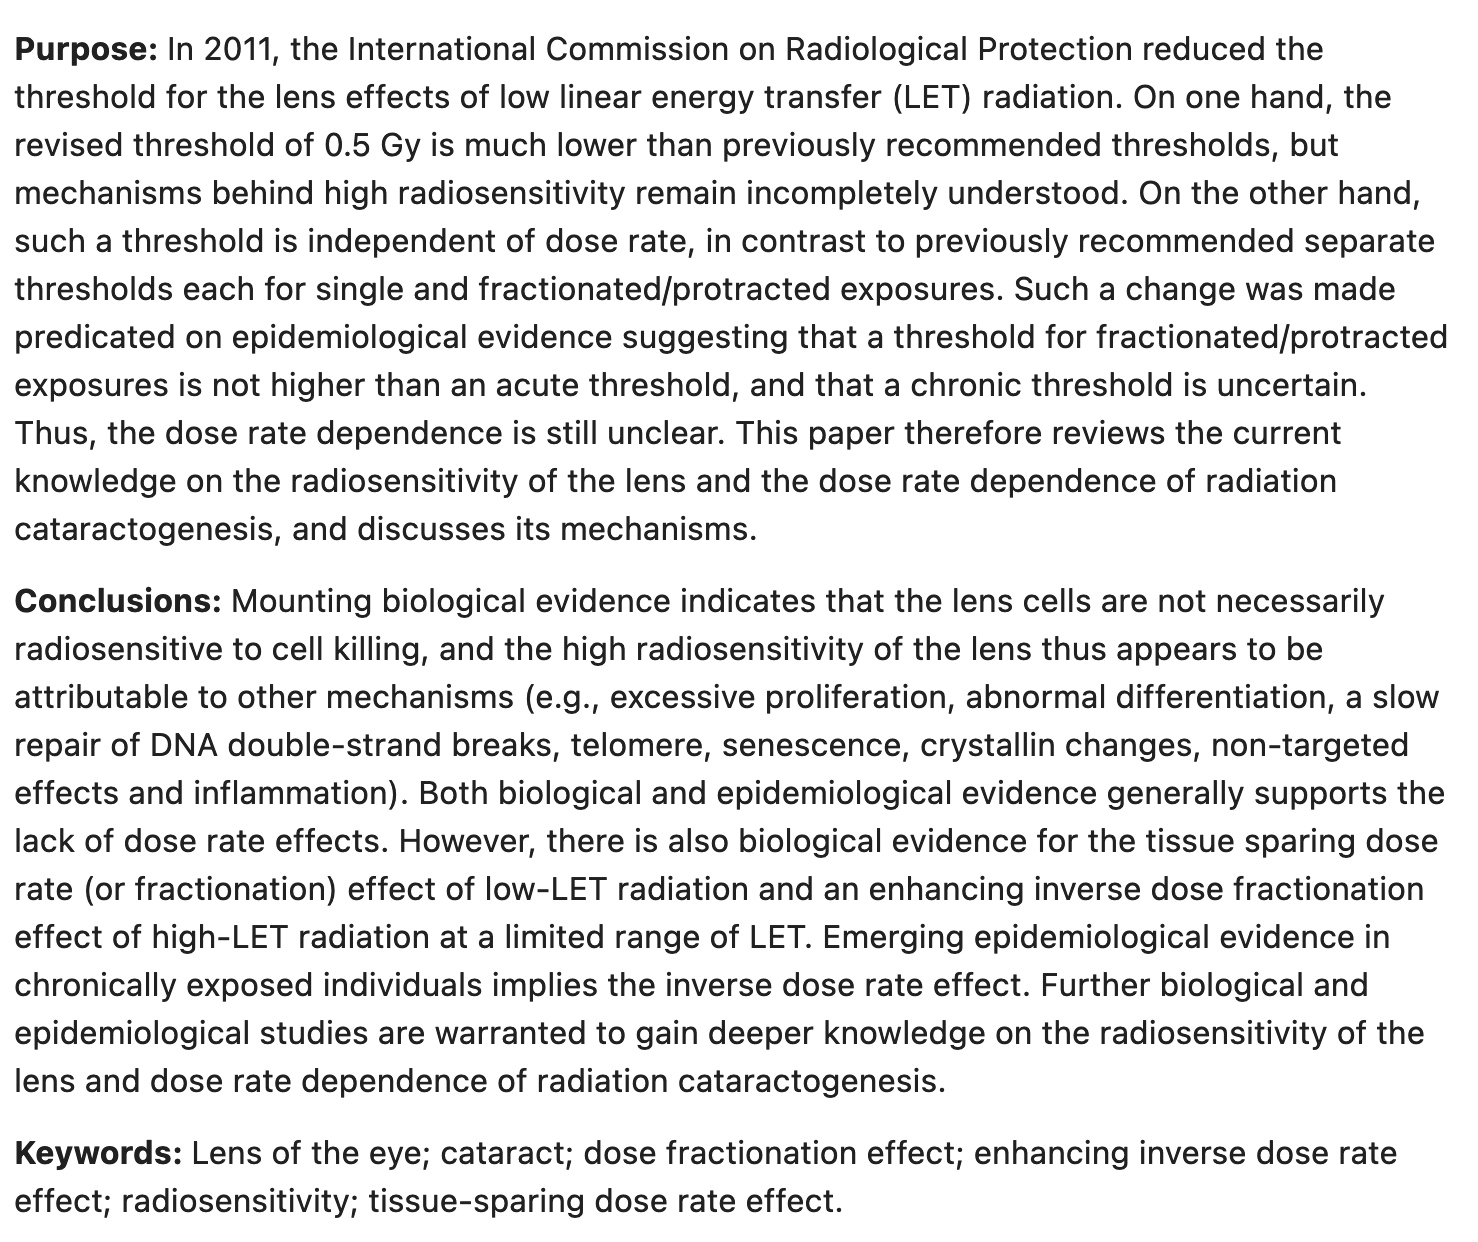
\includegraphics[scale=0.25]{images/hamada_2017_abstract.png}
   % 			\end{figure}
%\end{frame}


\subsection{CT Measurement Process Reviewed}

\begin{frame}
    \frametitle{Recap}
    \begin{itemize}
        \item Classical fan beam geometry:
    \end{itemize}
    \begin{figure}
        \centering{}
        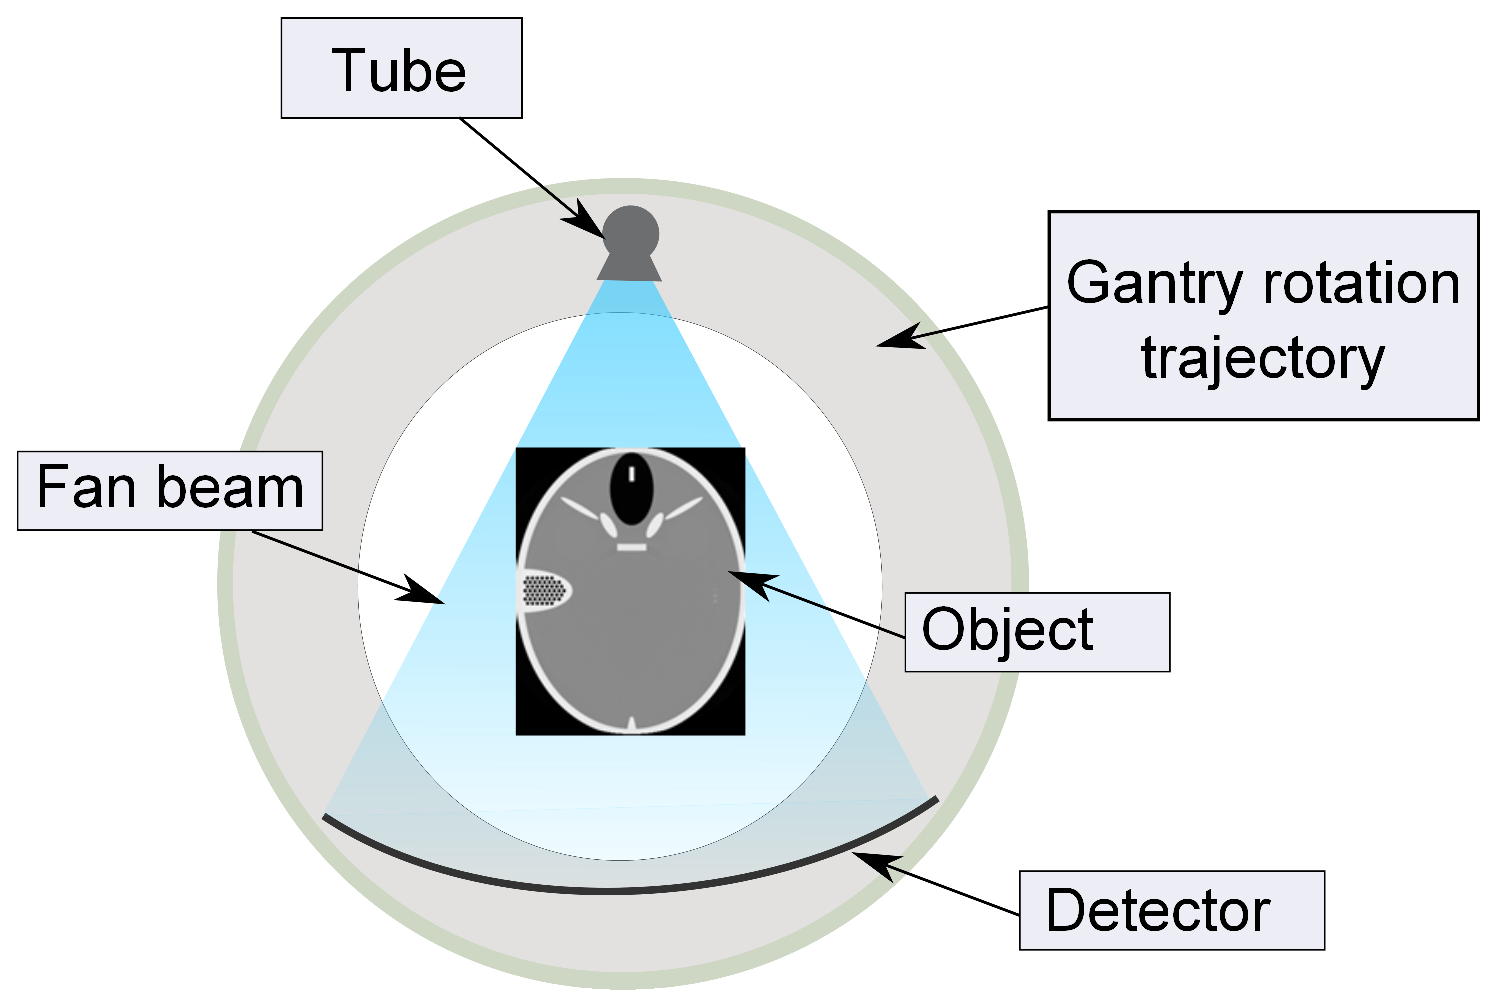
\includegraphics[scale=0.35]{images/multict.eps}
    \end{figure}
\end{frame}

\begin{frame}
    \frametitle{Sinogram}
    \begin{minipage}{0.52\textwidth}
        \begin{figure}
            \centering{}
            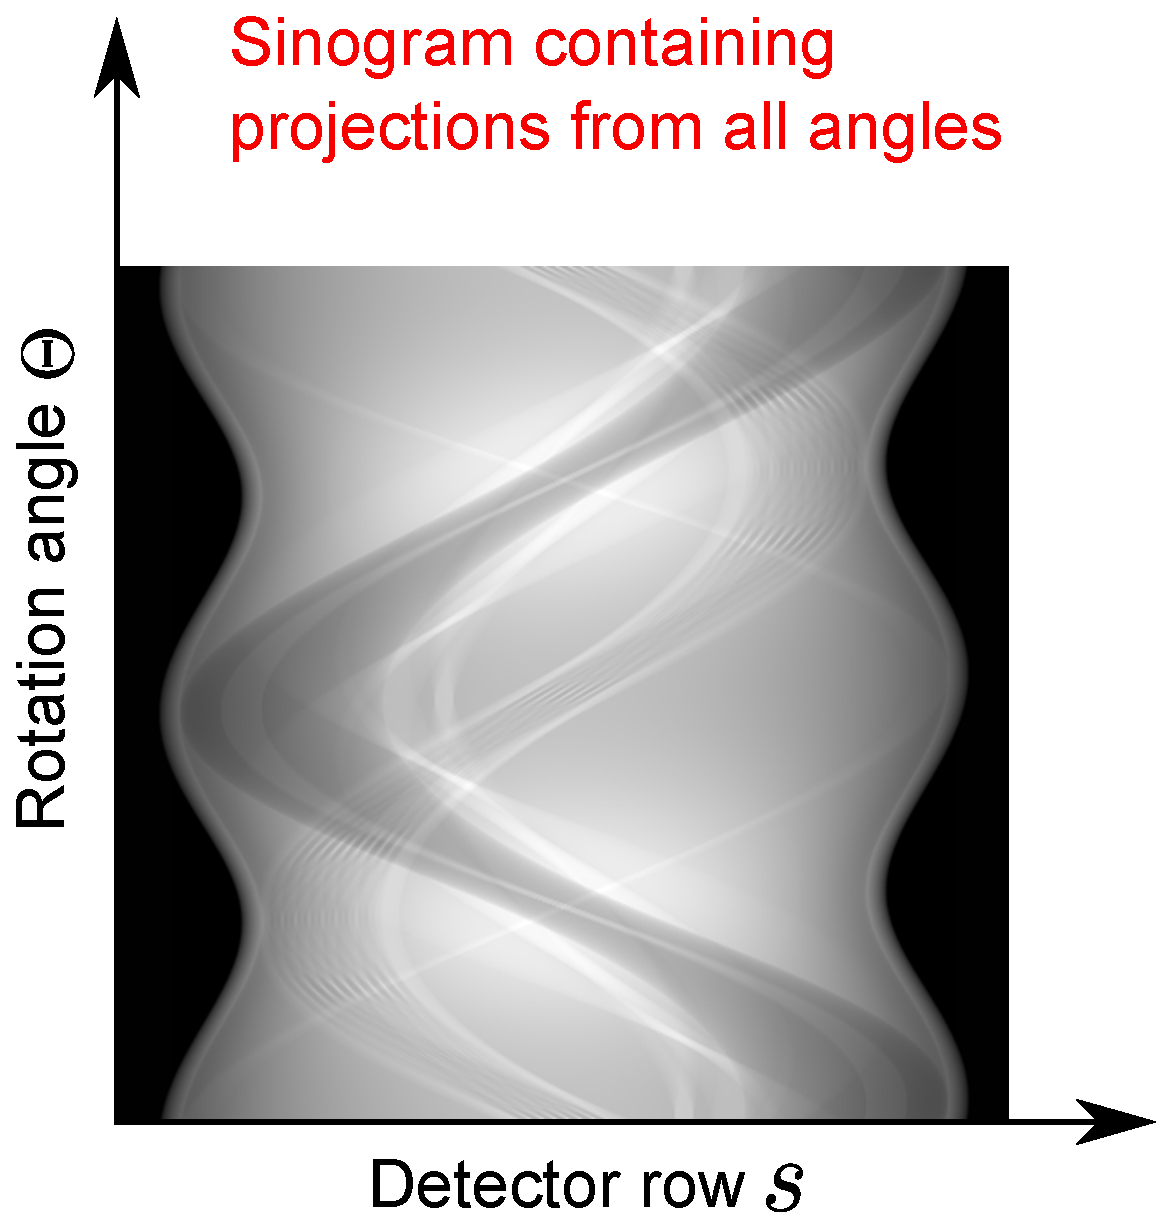
\includegraphics[scale=.30]{images/sinogram.eps}
        \end{figure}
    \end{minipage}
    \begin{minipage}{0.45\textwidth}
        \begin{figure}
            \centering{}
            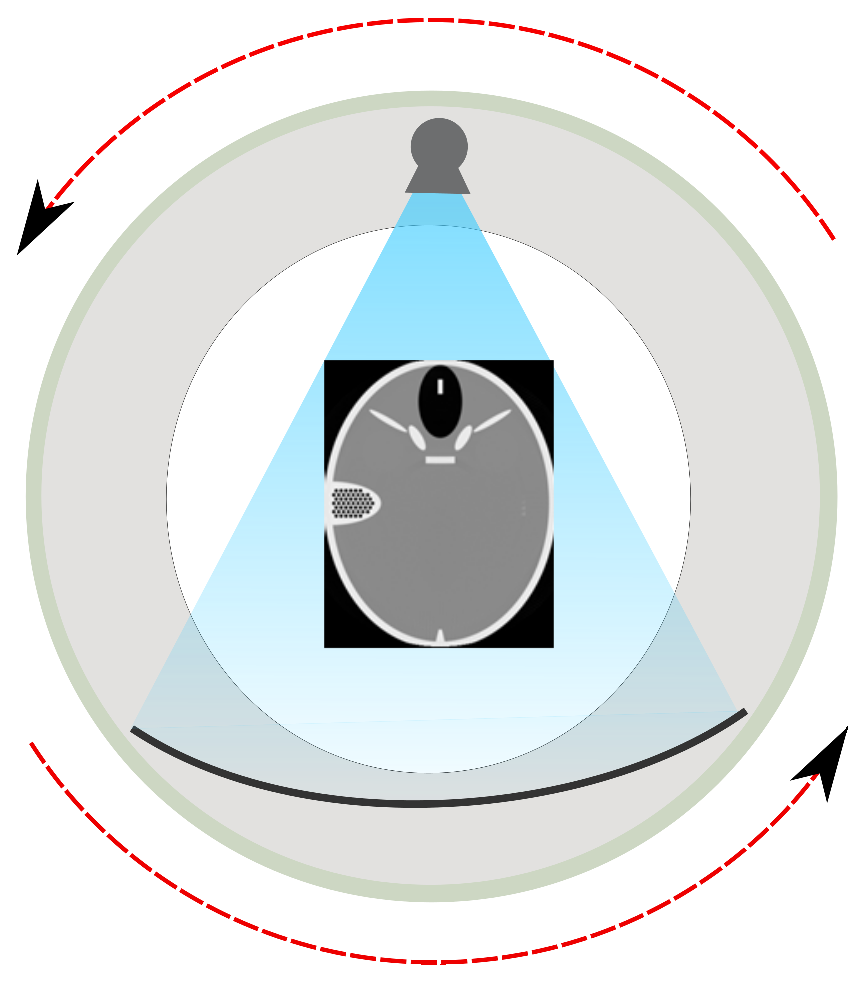
\includegraphics[scale=.35]{images/multict2.eps}
        \end{figure}
    \end{minipage}
\end{frame}

\begin{frame}{Projection Signal}

    \begin{columns}[c, onlytextwidth]
        \begin{column}{0.6\textwidth}
            Signal for single reading: \\
            \psfrag{ln}{{\LARGE $p(\Theta, s)$}}
            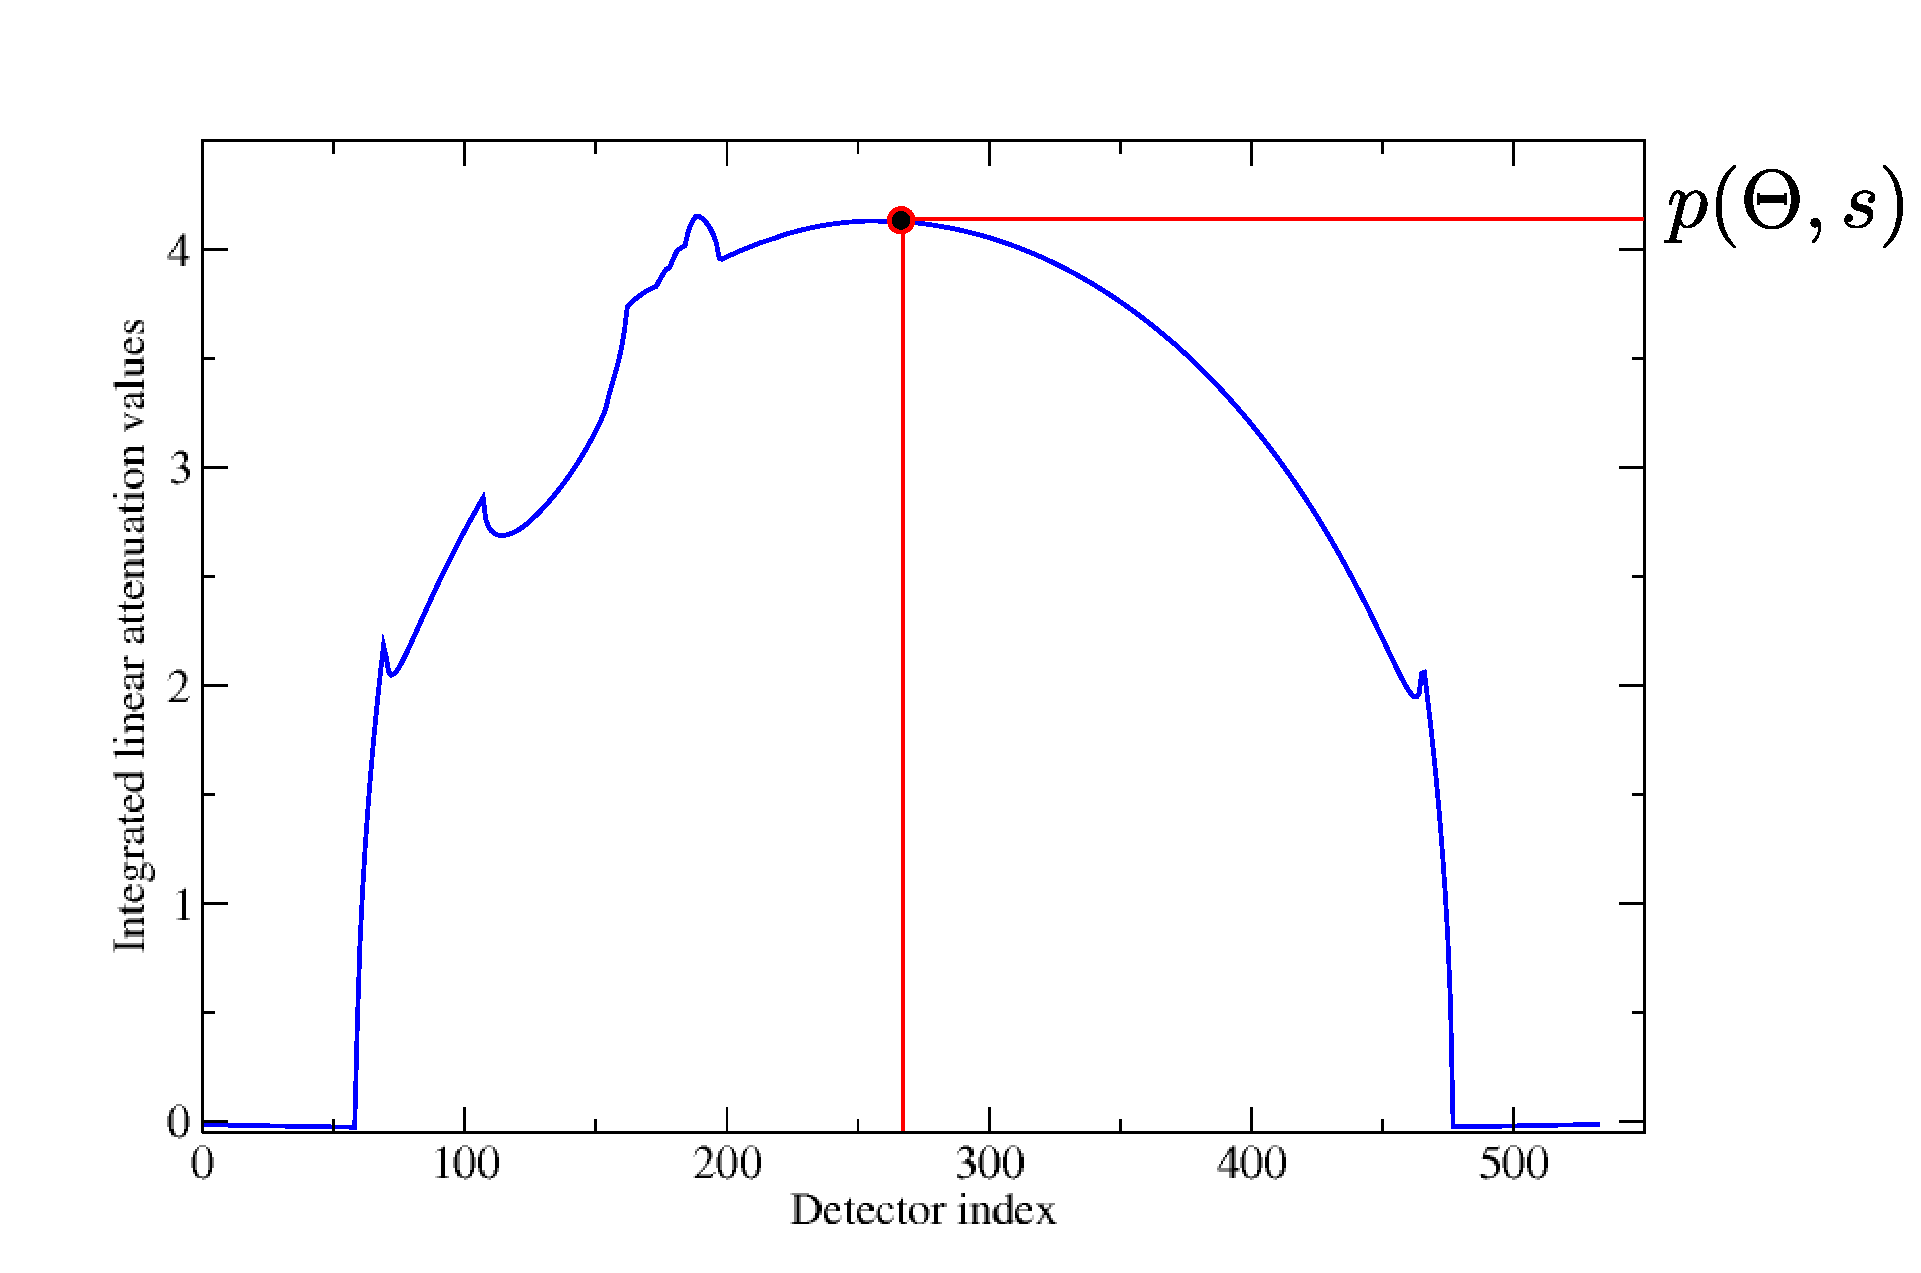
\includegraphics[width=0.8\textwidth]{images/projsig.eps}\\
            Measured intensity for a ray $l$:
            \begin{eqnarray*}
                p(\Theta, s) = \int{\mu}(l)dl
            \end{eqnarray*}
        \end{column}\begin{column}{0.4\textwidth}
            \begin{figure}
                \psfrag{l}{\LARGE{$\mu(l)$}}
                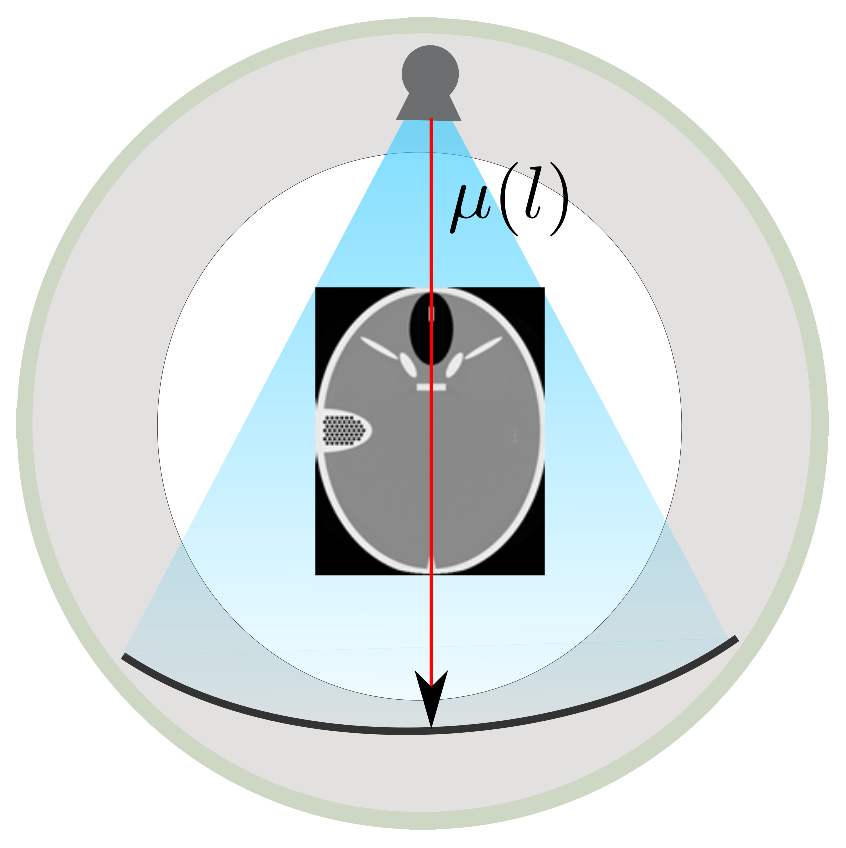
\includegraphics[width=0.8\textwidth]{images/multict3.eps}
            \end{figure}
        \end{column}
    \end{columns}
\end{frame}

\begin{frame}{Attenuation Law}
    \begin{align*}
        p^{\star}(\Theta, s)                               & = I_0 \cdot \exp\left(-\int	\mu(l)dl\right) \\
        -\ln\left(\dfrac{p^{\star}(\Theta, s)}{I_0}\right) & = p(\Theta, s) \tag{Radon transform}
    \end{align*}
    \begin{itemize}
        \item $p^{\star}(\Theta, s)$ denotes the measured X-ray intensity
        \item $I_0$ is the measured X-ray intensity without any attenuator
        \item $\mu(\vec x)$ is the \textit{linear attenuation coefficient} of the object at location $\vec x = (x ,y)$
        \item Reconstruction of $\mu(\vec x)$ from projections $p(\Theta, s)$\\ (e.\,g.\ by Iterative Reconstruction or Filtered Backprojection)
    \end{itemize}
\end{frame}

\begin{frame}
	\frametitle{Practical Considerations}

	\begin{itemize}
		\setlength\itemsep{0.5cm}
		\item \textcolor{faublue}{\textbf{So far:}} Theory and principles behind CT image reconstruction
		\item \textcolor{faublue}{\textbf{In practical applications}}: More aspects to consider\ldots
		      \begin{itemize}
			      \item Spatial resolution
			      \item Noise
			      \item Artifacts
		      \end{itemize}
	\end{itemize}

\end{frame}


\subsection{Spatial Resolution}

\begin{frame}
	\frametitle{Spatial Resolution}

	\begin{itemize}
		\setlength\itemsep{0.3cm}
		\item We may be interested in small structures (e.\,g.~vessels, calcifications)
		      \begin{itemize}
			      \item[$\Rightarrow$] High spatial resolution required
		      \end{itemize}
		\item Here, we will discuss resolution in the $x$-$y$ plane
		      \begin{itemize}
			      \item[ ] (In $z$-direction, it is governed by different factors)
		      \end{itemize}
		\item Resolution depends on several properties:
		      \begin{itemize}
			      \item Focus size $s_F$
			      \item Scan geometry ($r_F$: distance isocenter to focus, $r_D$ distance isocenter to detector center)
			      \item Detector element spacing $\Delta s$ and aperture $s_D$
			      \item Movement of focus and detector during acquisition
			      \item Reconstruction algorithm characteristics (summarized by factor $c_A$)
		      \end{itemize}
	\end{itemize}

\end{frame}

\begin{frame}
	\frametitle{Spatial Resolution}

	\begin{figure}
		\begin{center}
			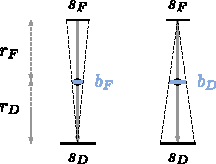
\includegraphics[width=0.5\linewidth]{images/resolution_3}
		\end{center}
		\caption{The effective sizes $b_F$ of the focus and $b_D$ of the detector in the isocenter can be calculated from the distances to the isocenter $r_F$ and $r_D$.}
		\label{fig:ct_resolution_3}
	\end{figure}

\end{frame}



\begin{frame}
	\frametitle{Spatial Resolution}

	\begin{itemize}
		\setlength\itemsep{0.3cm}
		\item From geometric setup, we determine blur measures $b_F$ and $b_D$:

		      \begin{eqnarray}
			      b_F &=& \frac{r_D}{r_F+r_D}\cdot s_F\\
			      b_D &=& \frac{r_F}{r_F+r_D}\cdot s_D
		      \end{eqnarray}

		\item Blur by continuous motion of focus and detector denoted by $b_M$
		\item Acquisition blur (determines maximum resolution):

		      \begin{equation}
			      b_{\textrm{acq}} = \sqrt{b_F^2+b_D^2+b_M^2}
		      \end{equation}

	\end{itemize}

\end{frame}

\begin{frame}
	\frametitle{Spatial Resolution}

	\begin{itemize}
		\setlength\itemsep{0.3cm}
		\item Blur by sampling and reconstruction:.
		\begin{itemize}
			\item $c_A$: Constant defined by the reconstruction algorithm.
			\item $\Delta s$: Detector element spacing.
		\end{itemize}
		      \begin{equation}
			      b_A = c_A \cdot \Delta s
		      \end{equation}


		\item Total blur:

		      \begin{equation}
			      b_{\textrm{total}} = \sqrt{b_F^2+b_D^2+b_M^2+b_A^2},
		      \end{equation}

		\item Limited influence as a user: Resolution is mainly defined by the system

	\end{itemize}

\end{frame}

\begin{frame}
	\frametitle{Measuring Spatial Resolution}

	\textcolor{faublue}{\textbf{Direct: Bar phantom}}
	\vspace{0.3cm}
	\begin{itemize}
		\setlength\itemsep{0.2cm}
		\item Contains lines of varying thickness
		\item How well are lines distinguishable after acquisition and reconstruction?
	\end{itemize}

	\vspace{0.5cm}
	\textcolor{faublue}{\textbf{Indirect (but more reliable): Thin wire phantom}}
	\vspace{0.3cm}
	\begin{itemize}
		\setlength\itemsep{0.2cm}
		\item Measurement yields the point spread function (PSF)
		\item Fourier transform of PSF is known as modulation transfer function (MTF)
		\item Frequency typically measured in line pairs per cm
		\item Characteristic value: Frequency at 10\% original contrast
	\end{itemize}

\end{frame}

\begin{frame}
	\frametitle{Measuring Spatial Resolution}

	\begin{figure}
		\begin{center}
			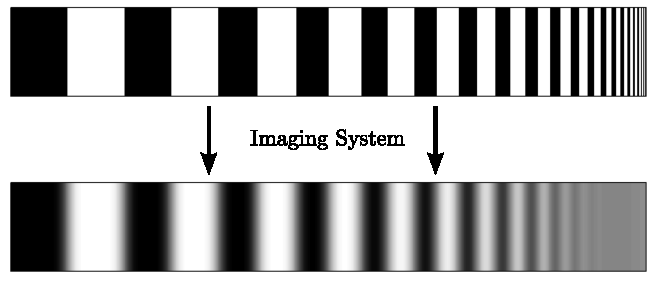
\includegraphics[width=0.6\linewidth]{images/resolution_2}
		\end{center}
		\caption{A bar phantom can be used to evaluate the spatial resolution of an imaging system. At sufficiently high spatial frequencies, individual lines can no longer be separated after imaging, i.\,e.~we have determined the system's resolution limit.}
		\label{fig:ct_resolution_2}
	\end{figure}

\end{frame}



\begin{frame}
	\frametitle{Measuring Spatial Resolution}

	\begin{figure}
		\begin{center}
			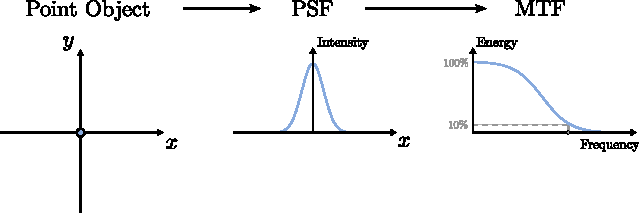
\includegraphics[width=0.9\linewidth]{images/resolution_1}
		\end{center}
		\caption{If we could scan an ideal point object, the resulting reconstructed image would be the PSF of the system. The Fourier transform of the PSF is the MTF, which shows the relative contrasts achievable for varying object frequencies. In practice, this measurement is typically  performed using thin wire phantoms.}
		\label{fig:ct_resolution_1}
	\end{figure}

\end{frame}

\subsection{Noise}


\begin{frame}[allowframebreaks]
	\frametitle{Noise}

	\begin{itemize}
		\item We know: number of measured photons $n_s$ is Poisson distributed with
		      $E[n_s] = N_0 p_a$
		      \begin{itemize}
			      \item $N_0$: expected value of no. of photons generated
			      \item $p_a$: probability of a photon passing through object unaffected
		      \end{itemize}
		\item Approximate Poisson process by Gaussian with $\mu = E[n_s]$ and $\sigma = \sqrt{E[n_s]}$ (valid for large no. of photons)

		\item Conversion to line integrals involves taking negative logarithm:

		      \begin{equation}
			      \int \mu(s) \textnormal ds = -\ln\frac{I}{I_0},
		      \end{equation}

		      where $\frac{I}{I_0} = \frac{N_0 p_a}{N_0} = p_a$
		\item New approx.~distribution has $\mu = -\ln p_a$ and $\sigma = \frac{1}{\sqrt{N_0 p_a}}$
		\item Note: Noise variance increases with object thickness

		\item Back-projection step computes weighted sum of (filtered) values
		\item[ ] $\Rightarrow$ Object dependence of noise statistics propagates into 3-D
		\item In non-circular objects, streak structures appear in the noise
	\end{itemize}

	\begin{figure}
		\begin{center}
			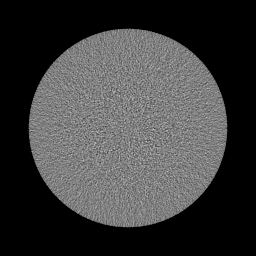
\includegraphics[width=0.25\linewidth]{images/noise1}
			\hspace{1cm}
			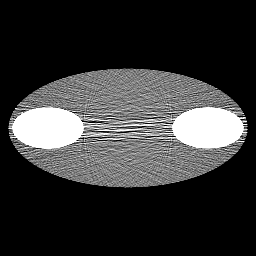
\includegraphics[width=0.25\linewidth]{images/noise2}
		\end{center}
		\caption{The left image shows the reconstruction of a water cylinder phantom. The noise is stronger in the center than in the peripheral regions. On the right side, an elliptic phantom with two high intensity insets is depicted. In its center, streak noise emerges that is caused by the strongly attenuating structures. For both phantom simulations, $90{,}000$ photons per pixel with an energy of $75$ keV were used.}%
		\label{fig:ct_noise}
	\end{figure}

\end{frame}

\subsection{Artifacts}

\begin{frame}
	\frametitle{Artifacts}

	Common artifacts:

	\begin{itemize}
		\setlength\itemsep{0.3cm}
		\item Beam Hardening
		\item Scatter Artifacts
		\item Partial Volume Effect
		\item Metal Artifacts
		\item Motion Artifacts
		\item Truncation Artifacts
	\end{itemize}

\end{frame}

\begin{frame}
	\frametitle{Beam Hardening}
	Practically used X-ray sources are polychromatic
 	\begin{center}\includegraphics[height=0.8\textheight ]{images/phxray2-eps-converted-to}\end{center}
\end{frame}

\begin{frame}
	\frametitle{Beam Hardening}

	\begin{itemize}
		\setlength\itemsep{0.3cm}
		\item Practically used X-ray sources are polychromatic
		      \begin{itemize}
			      \item[$\Rightarrow$] Attenuation of homogeneous object not proportional to thickness along ray
		      \end{itemize}
		\item Wide, continuous spectrum of energies
		\item But: attenuation coefficients are energy dependent
		\item Lower energy photons are more easily absorbed
		      \begin{itemize}
			      \item[$\Rightarrow$] Shift to higher energies (``beam hardening'')
			      \item[$\Rightarrow$] Streak and cupping artifacts
		      \end{itemize}
		\item Common approach: Pre-filter X-rays to absorb low energy photons
	\end{itemize}

\end{frame}

\begin{frame}[t]{Beam Hardening}
	\begin{figure}[htpb]
		\centering
		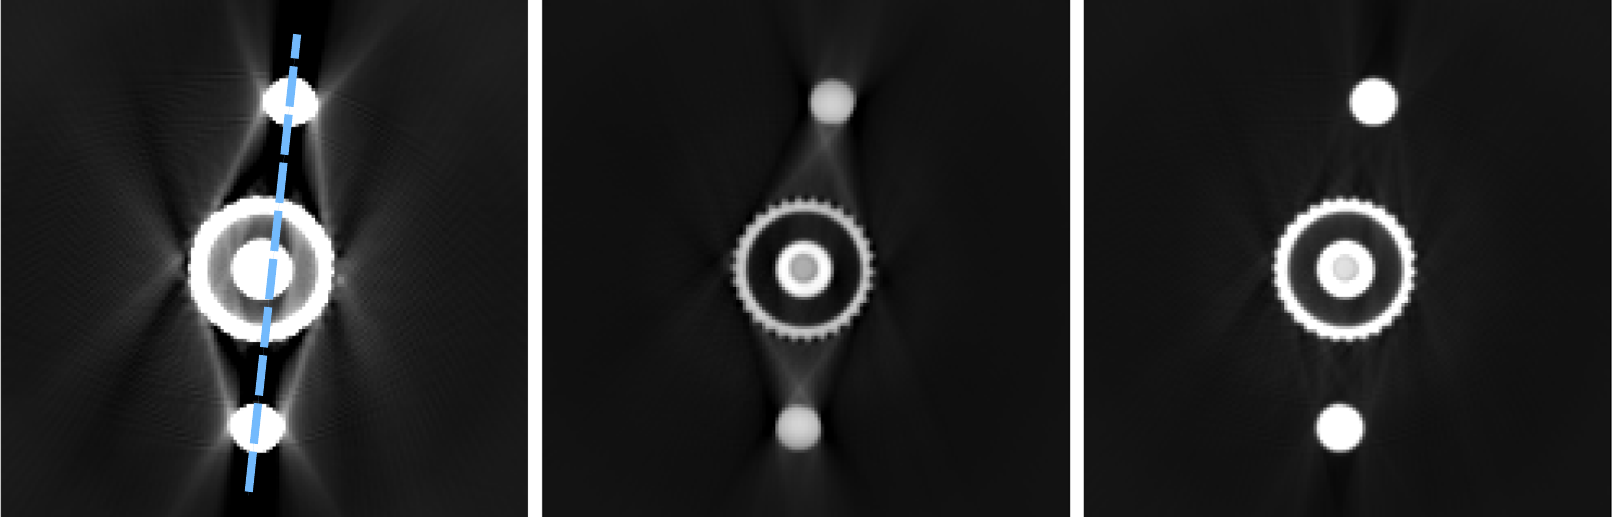
\includegraphics[height=0.6\textheight]{images/beam_hardening.png}
		\caption{Beam hardening on a watch dataset. From left to right: Watch dataset reconstructed; Beam hardening reduced using the TV method; Beam hardening reduced using our proposed method. (Window: C/W = 0.092/0.183).}%
	\end{figure}
	\flushright{}
	\tiny
	\fullcite{wuerfel_beam_hardening}
\end{frame}

\begin{frame}
	\frametitle{Scatter Artifacts}
	\begin{columns}[c, onlytextwidth]
		\begin{column}{0.75\textwidth}
		\begin{itemize}
			\item Scattered photons change direction and energy
			\item[ ] $\Rightarrow$ Measured in different location
			\item Large effect when it hits element with few ``regular'' photons

			\item Cupping and streak artifacts (esp.\ between high density structures)
		
		\end{itemize}
		\end{column}
		\begin{column}{0.25\textwidth}
		 \begin{figure}
			\centering
			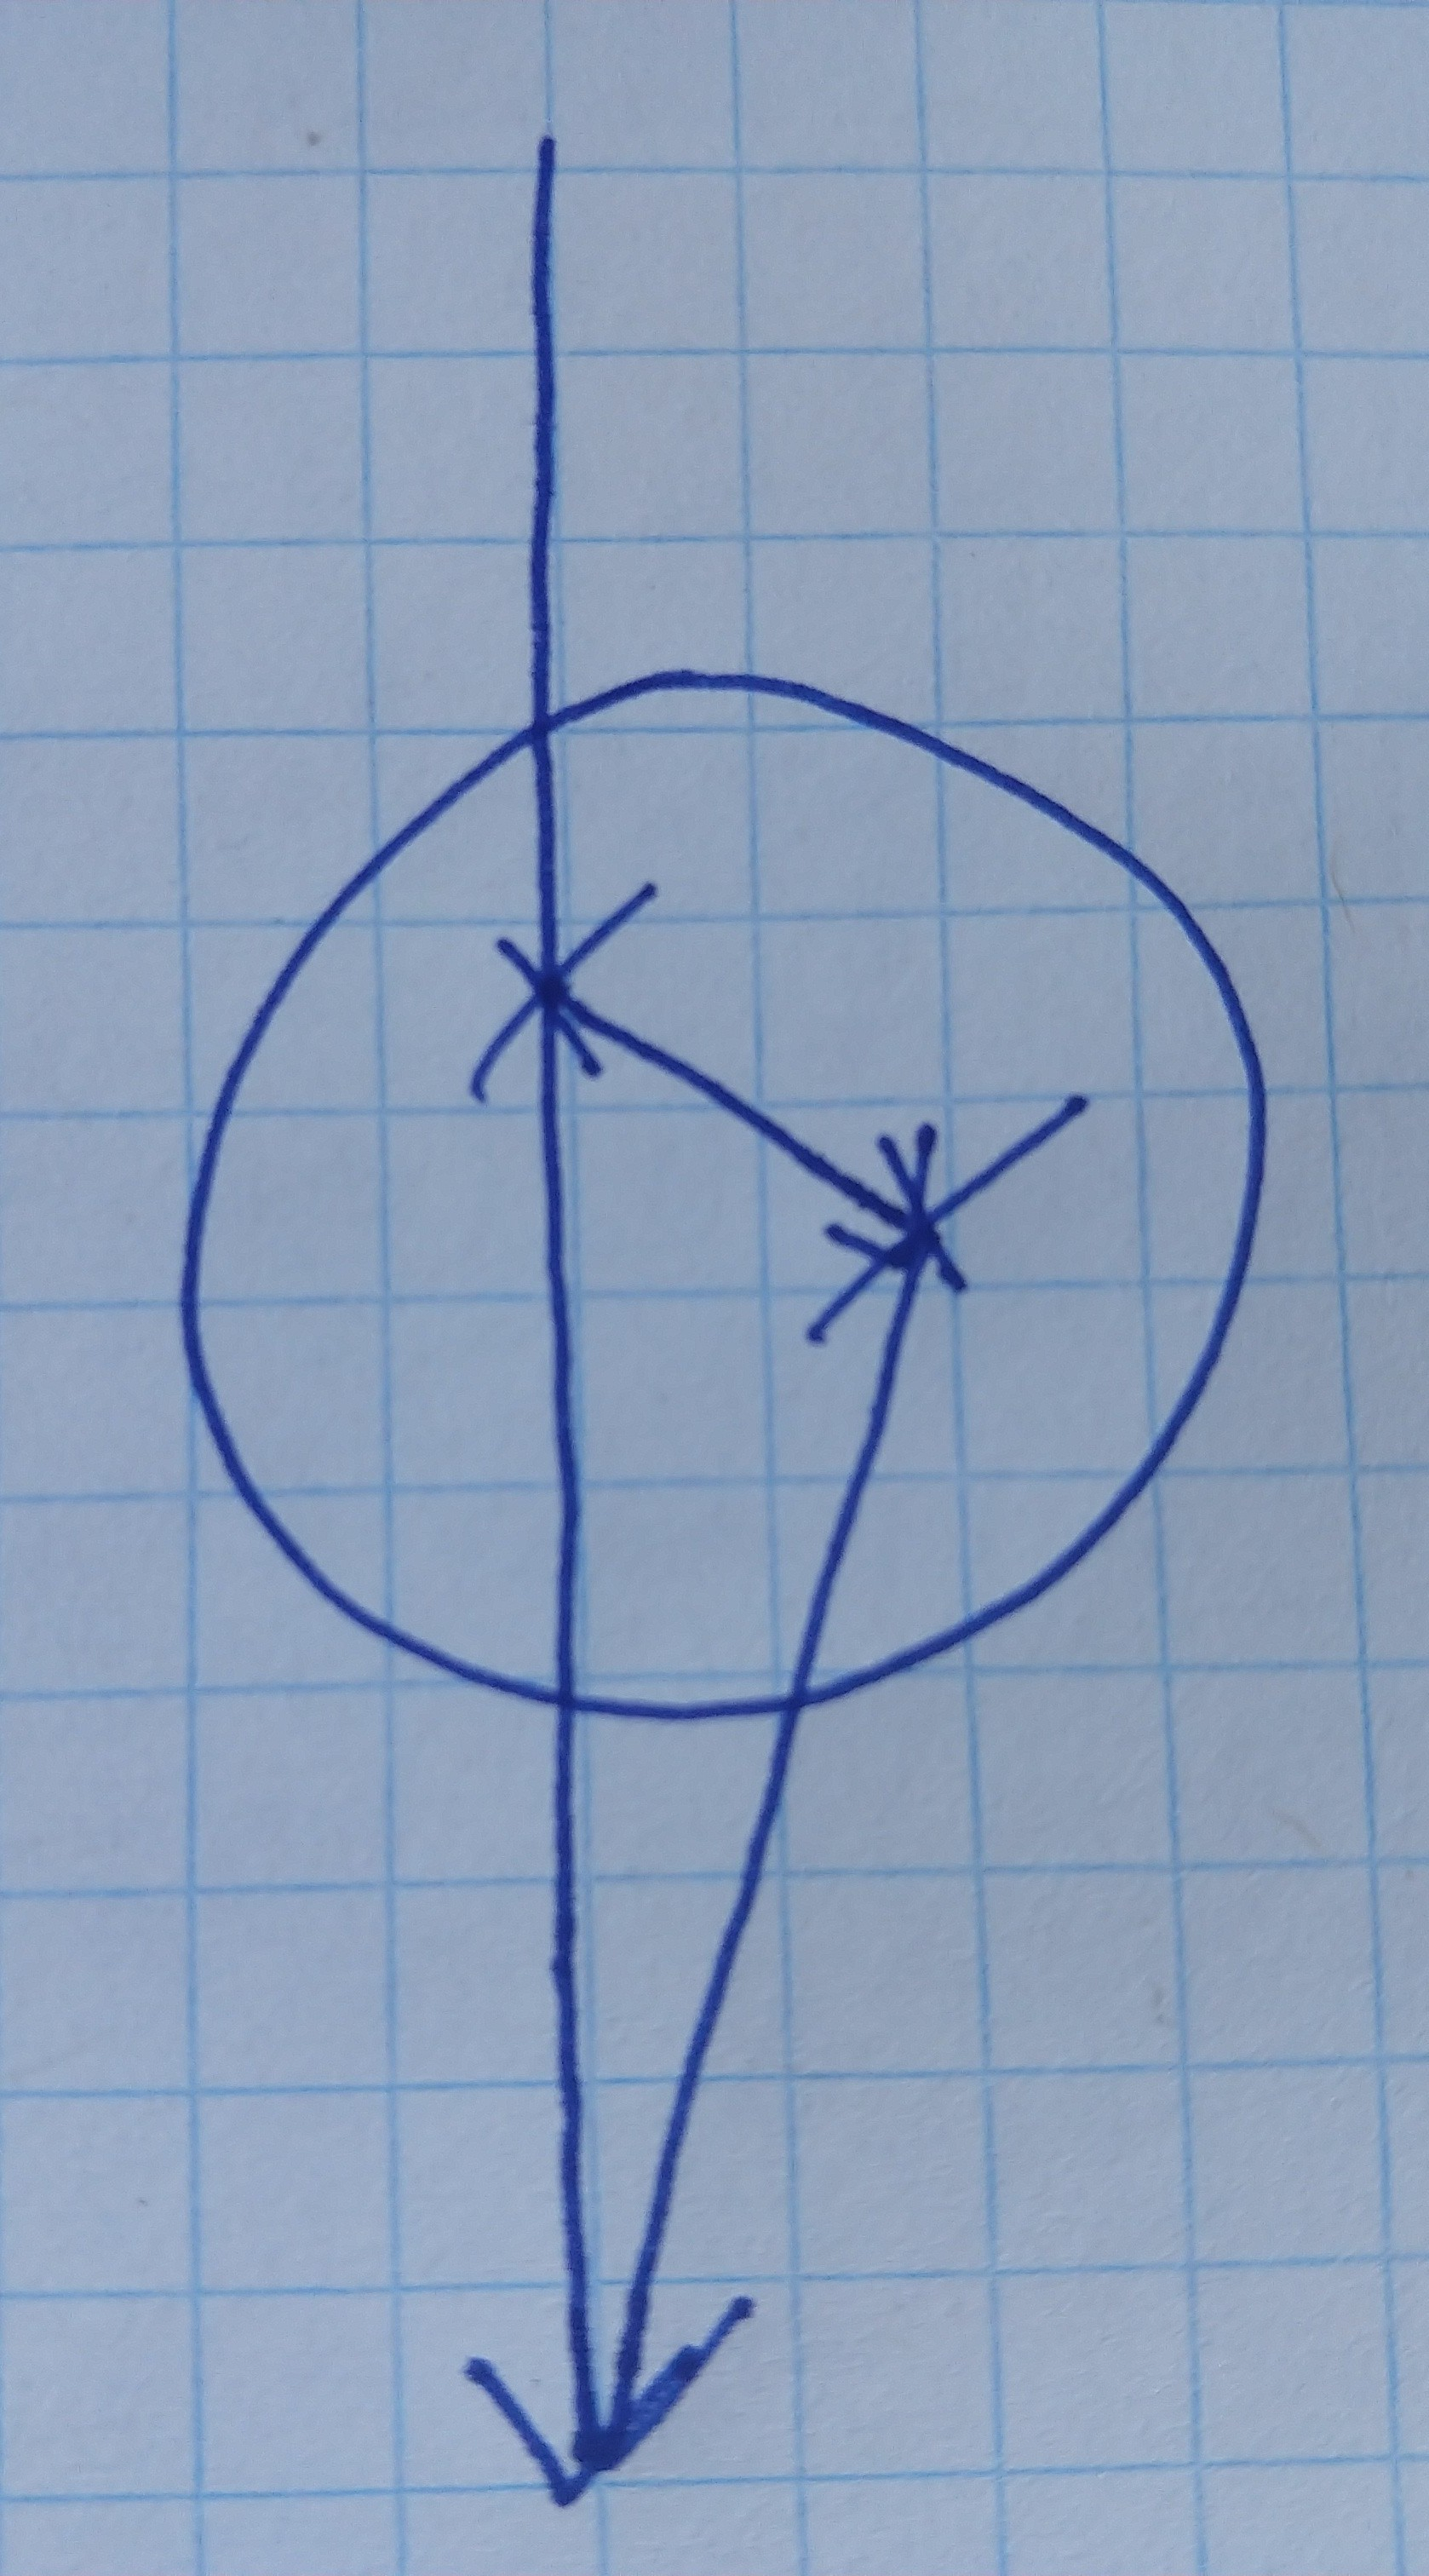
\includegraphics[height=0.75\textwidth]{images/scatter_sketch}
		 \end{figure}
	\end{column}
	\end{columns}

\end{frame}
	
	\begin{frame}
	\frametitle{Scatter Artifacts}
	\begin{columns}[c, onlytextwidth]
		\begin{column}{0.75\textwidth}
		\begin{itemize}
			\item Scattered photons change direction and energy
			\item[ ] $\Rightarrow$ Measured in different location
			\item Large effect when it hits element with few ``regular'' photons

			\item Cupping and streak artifacts (esp.\ between high density structures)
			\item Most scanners use anti-scatter grids:
		\end{itemize}
		\end{column}
		\begin{column}{0.25\textwidth}
		 \begin{figure}
			\centering
			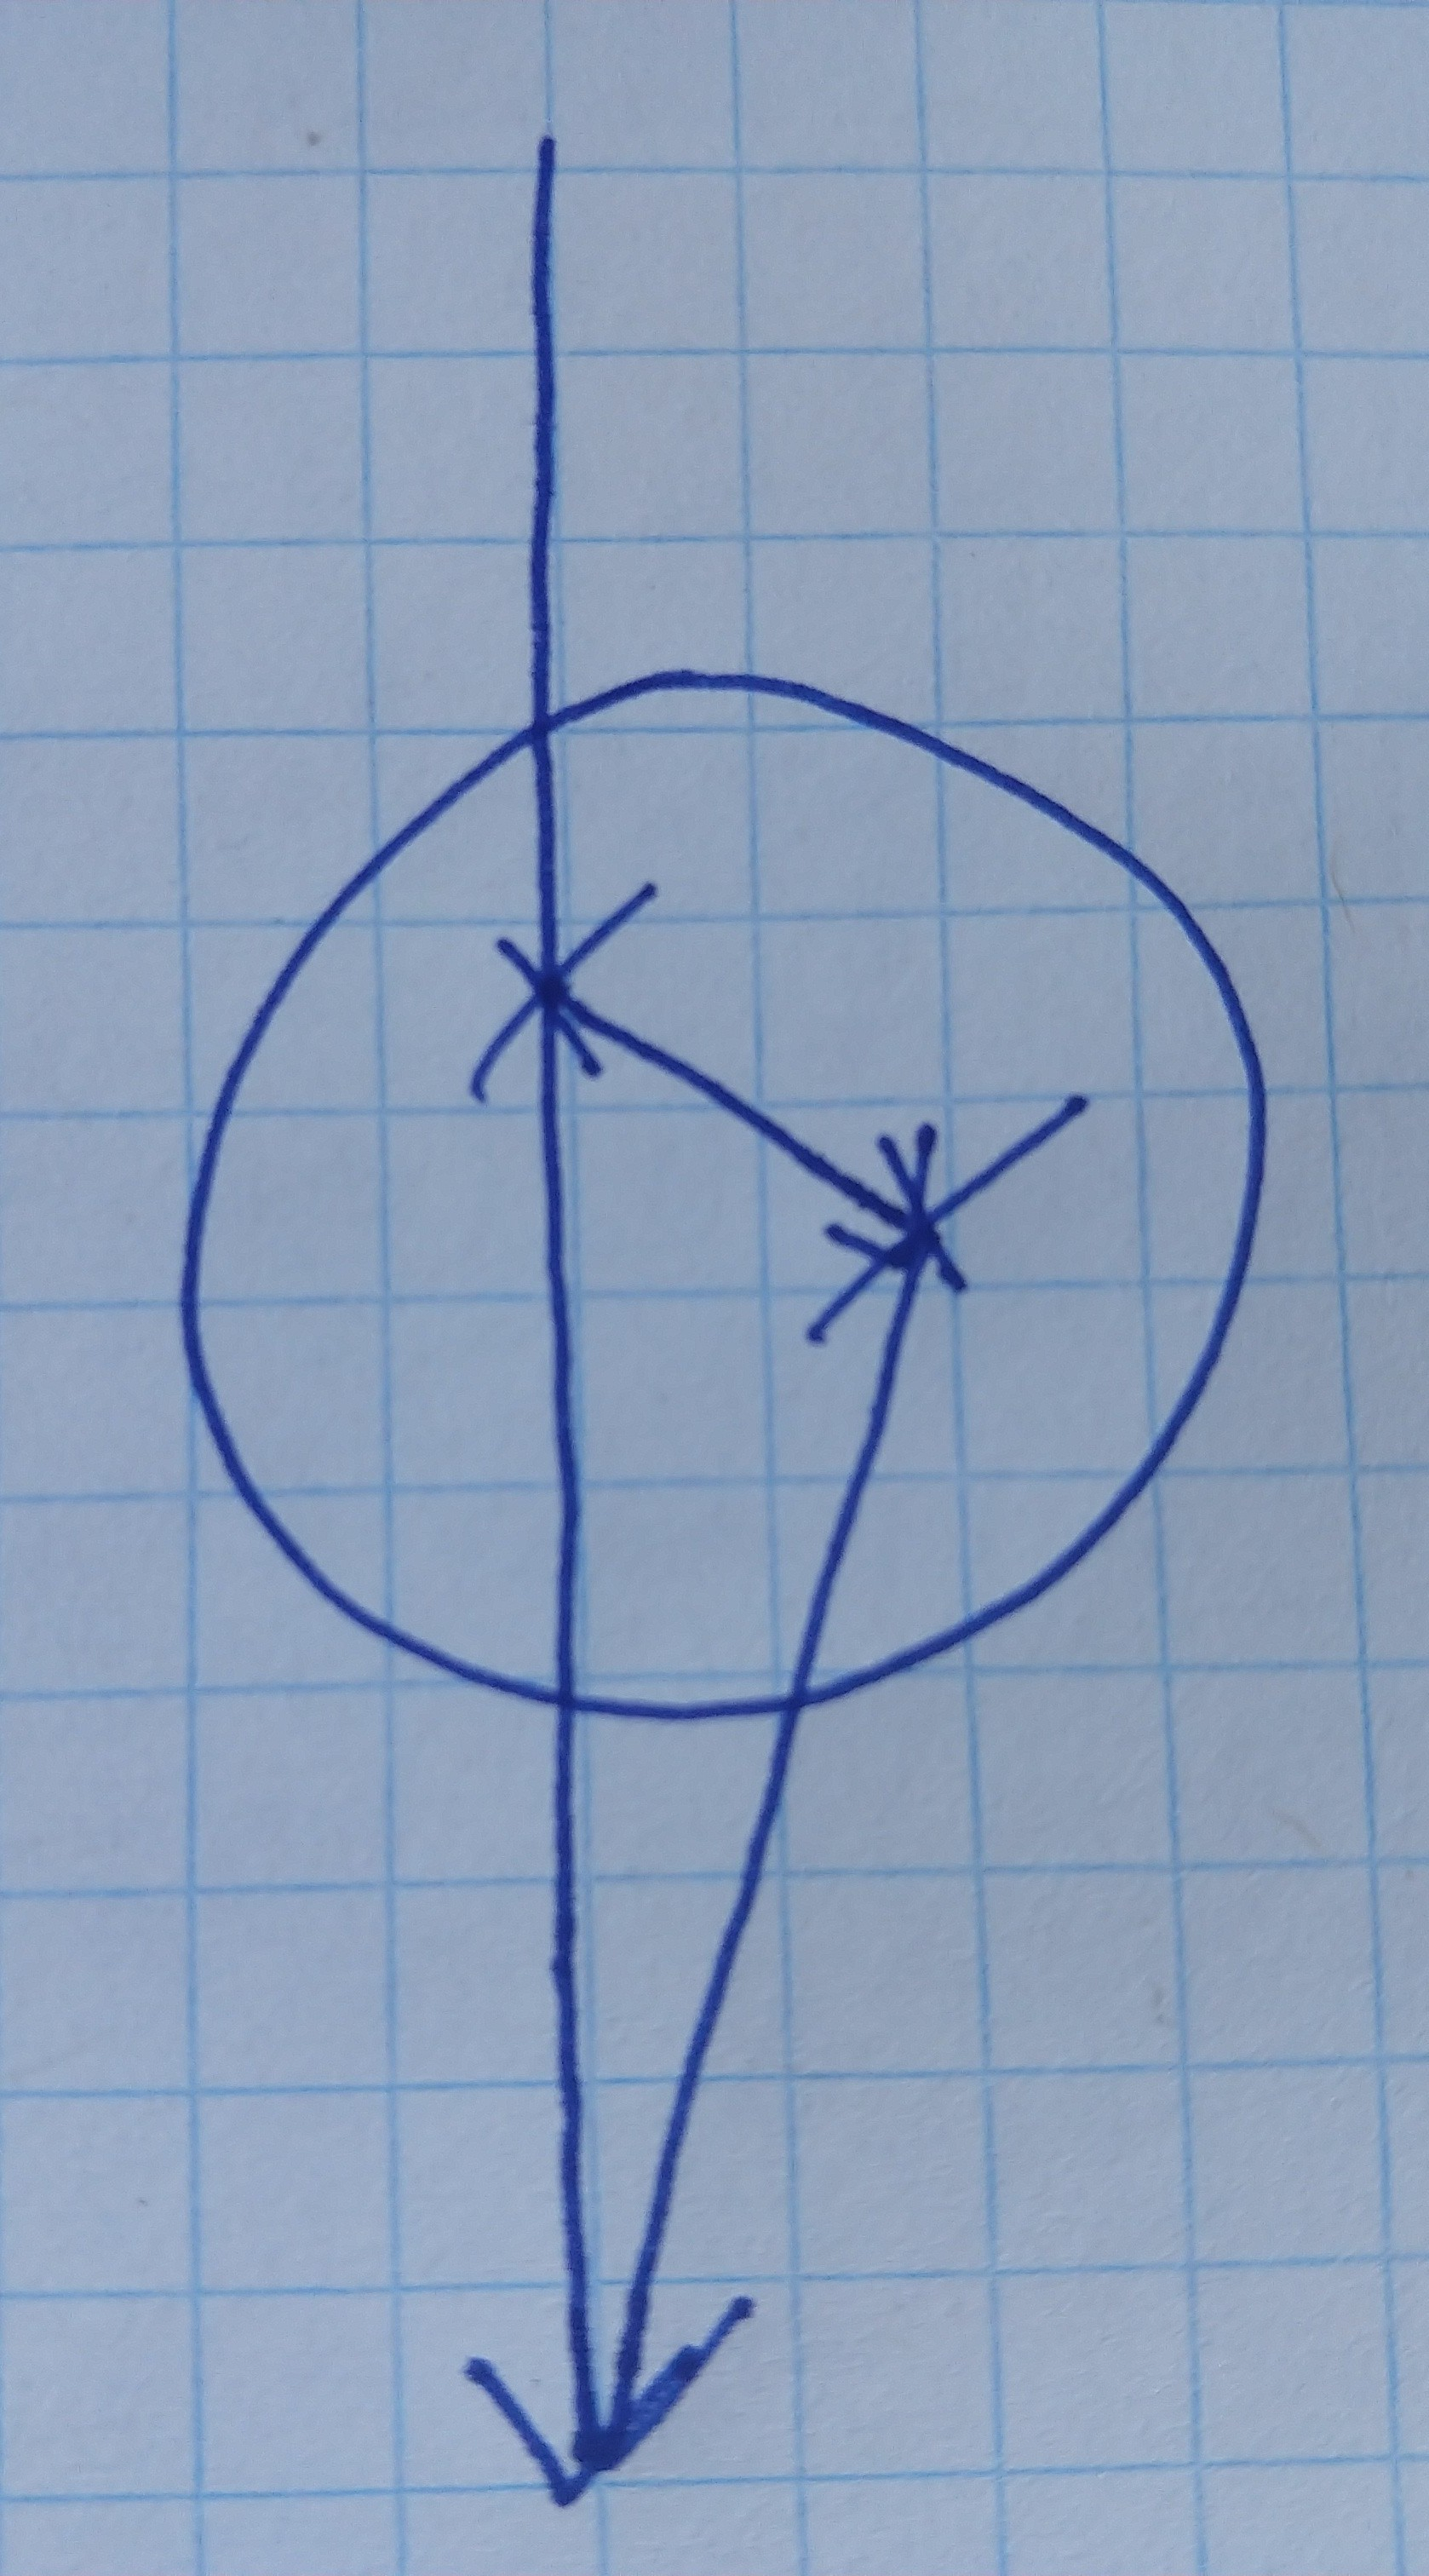
\includegraphics[height=0.75\textwidth]{images/scatter_sketch}
		 \end{figure}
	\end{column}
	\end{columns}

	\begin{figure}
		\centering
		\includegraphics[width=0.45\linewidth]{images/scatter_1}
		\caption{Anti-scatter grids can be placed in front of the detector to reject scattered radiation.}
		\label{fig:ct_scatter_1}
	\end{figure}

\end{frame}

\begin{frame}[c]{Scatter Artifacts}
	\begin{figure}[]
		\centering
		\begin{columns}[t, onlytextwidth]
			\begin{column}{0.25\textwidth}
				\centering{}
				\includegraphics[width=0.8\linewidth]{images/scatter_primary.png}\\
				Primary
			\end{column}\begin{column}{0.25\textwidth}
				\centering{}
				\includegraphics[width=0.8\linewidth]{images/scatter_rayleigh.png}\\
				Rayleigh
			\end{column}\begin{column}{0.25\textwidth}
				\centering{}
				\includegraphics[width=0.8\linewidth]{images/scatter_compton.png}\\
				Compton
			\end{column}\begin{column}{0.25\textwidth}
				\centering{}
				\includegraphics[width=0.8\linewidth]{images/scatter_multiple.png}\\
				Multiple
			\end{column}
		\end{columns}
	\end{figure}
	\flushright{}
	\small Simulated scattering artifacts on projections

	Different intensity scales, primary is by far the strongest
\end{frame}

%\begin{frame}[c]{Scatter Artifacts}
%\begin{figure}[htpb]
%\centering
%\includegraphics[height=0.8\textheight]{images/scatter_joscha_maier.png}
%%\caption{Scatter needs to be compensated for}%
%\end{figure}

%%\vspace{-1cm}
%\flushright
%\tiny
%\fullcite{joscha_dse}

%\end{frame}

\begin{frame}[c]{Scatter Artifacts}
	\begin{figure}[htpb]
		\centering
		\includegraphics[height=0.55\textheight]{images/bier_scatter_correction_with_labels.png}
		\caption{Reconstructed imagesof a elliptical Electron Density Phantom with and without scatter correction. Grayscale window: C = 0 HU, W = 2000 HU.}%
	\end{figure}

	\vspace{0.5cm}
	\flushright{}
	\tiny
	\fullcite{bier17}

\end{frame}



\begin{frame}[allowframebreaks]
	\frametitle{Partial Volume Effect}
	\hspace{-0.3cm}

	\begin{itemize}
		\item Mostly in low resolution images, not often seen in state-of-the-art CT
		\item One pixel spans two regions with different absorption coeffs.~$\mu_1$, $\mu_2$
		\item First case:
		      \begin{eqnarray}
			      I_1 \cdot e^{-\mu_1\Delta x},\\
			      I_2 \cdot e^{-\mu_2\Delta x},
		      \end{eqnarray}
		      where $I_1 + I_2 = I_0$. Measured intensity:
		      \begin{equation}
			      \label{eq:ct_partial1}
			      I_x = I_1 \cdot e^{-\mu_1\Delta x} + I_2 \cdot e^{-\mu_2 \Delta x},
		      \end{equation}

		\item This differs from the expected average absorption:
		      \begin{eqnarray}
			      I &=& I_0 \cdot e^{- \frac{1}{2}(\mu_1 + \mu_2) \Delta x} =\\
			      &=& I_1 \cdot e^{- \frac{1}{2}(\mu_1 + \mu_2) \Delta x} + I_2 \cdot e^{- \frac{1}{2}(\mu_1 + \mu_2) \Delta x} \neq I_x.
		      \end{eqnarray}

		\item Second case (matches average absorption):
		      \begin{eqnarray}
			      I_y &=& I_1 \cdot e^{-\mu_1\Delta\frac{y}{2} - \mu_2\Delta\frac{y}{2}} +I_2 \cdot e^{-\mu_1\Delta\frac{y}{2} - \mu_2\Delta\frac{y}{2}} = \\
			      &=& (I_1 + I_2) \cdot e^{-\mu_1\Delta\frac{y}{2} - \mu_2\Delta\frac{y}{2}} =\\
			      &=& I_0 \cdot e^{-\frac{1}{2}(\mu_1 + \mu_2)\Delta y} \neq I_x,
		      \end{eqnarray}
		\item[ ] $\Rightarrow$ Streak artifacts due to inconsistent measurements

	\end{itemize}

\end{frame}
\begin{frame}
	\frametitle{Partial Volume Effect}

	\begin{figure}[tbp]
		\centering
		\includegraphics[height=0.7\textheight]{images/schwemmer_partial_volume.jpg}
		\caption{Cross-sectional vessel profile views. Shown are centreline point (blue cross), estimated actual centre (red cross), detected vessel borders (green dots) and estimated vessel diameter (white dots).}%
		\label{fig:ct_partial_1}
	\end{figure}
	\vspace{-0.5cm}

	\flushright{}
	\tiny
	\fullcite{schwemmer14}

\end{frame}

\begin{frame}
	\frametitle{Metal Artifacts}

	%\begin{figure}
	%       \centering
	%       %\includegraphics[width=0.9\linewidth]{images/metal_1}
	%       \caption{Photon starvation due to metallic objects can lead to streak artifacts in the reconstructed image.}
	%       \label{fig:ct_metal_1}
	%\end{figure}

	\begin{itemize}
		\setlength\itemsep{0.3cm}
		\item One of the most common image artifacts in CT
		\item Covers different types of artifacts we already discussed
		\item Metal causes beam hardening and scatter
		      \begin{itemize}
			      \item[$\Rightarrow$] dark streaks between metal objects
		      \end{itemize}
		\item Strong attenuation $\Rightarrow$ photon starvation $\Rightarrow$ noisy projections

		\item Possible solutions:
		      \begin{itemize}
			      \item Increased tube current or automatic current modulation
			      \item Metal artifact reduction algorithms (e.\,g.~remove metal objects in reconstruction, iteratively interpolate holes in forward projection)
		      \end{itemize}

	\end{itemize}
\end{frame}

\begin{frame}[c]{Metal Artifacts}
	\begin{figure}[tbp]
		\centering
		\includegraphics[height=0.5\textheight]{images/herl_metal_artifacts.jpg}
		\caption{Multipositional data fusion with smART metal artifact reduction algorithm (c) from scans (a) and (b)}%
		\label{fig:metal_arifatc_reduction}
	\end{figure}
	%\vspace{1.3cm}

	\flushright{}
	\tiny
	\fullcite{herl_metal_artifacts}

\end{frame}

\begin{frame}
	\frametitle{Motion Artifacts}

	\begin{itemize}
		\setlength\itemsep{0.3cm}
		\item (Cardiac, respiratory) motion during acquisition: inconsistent projections
		\item[$\Rightarrow$] Blurring or streak artifacts
		\item Prevalent in C-arm (cone beam) CT due to the slow rotation speed
		\item Can be reduced by estimating motion and correcting for it during reconstruction (motion compensation)

	\end{itemize}

\end{frame}


\begin{frame}
	\frametitle{Motion Artifacts}

	\begin{figure}[tbp]
		\centering
		\includegraphics[height=0.7\textheight]{images/motion_1}
		\hspace{1cm}
		\includegraphics[height=0.7\textheight]{images/motion_2}
		\caption{An image of human legs reconstructed from motion-corrupted projections using regular filtered back-projection (left) and with an additonal marker-based correction (right). By compensating for motion during reconstruction, structures that were originally blurred due to the movement become visible and streak artifacts caused by misalignments are reduced considerably.}%
		\label{fig:ct_motion}
	\end{figure}

\end{frame}

%\begin{frame}
%	\frametitle{Motion Artifacts}

%	\begin{figure}[tbp]
%		\centering
%		\includegraphics[height=0.7\textheight]{images/motion_1}
%		\hspace{1cm}
%		\includegraphics[height=0.7\textheight]{images/motion_2}
%		\caption{An image of human legs reconstructed from motion-corrupted projections using regular filtered back-projection (left) and with an additonal marker-based correction (right). By compensating for motion during reconstruction, structures that were originally blurred due to the movement become visible and streak artifacts caused by misalignments are reduced considerably.}%
%		\label{fig:ct_motion2}
%	\end{figure}

%\end{frame}

\begin{frame}
	\frametitle{Truncation Artifacts}
	\begin{columns}[c, onlytextwidth]
		\begin{column}{0.65\textwidth}
		\begin{itemize}
		\setlength\itemsep{0.3cm}
		\item Scanned object larger than detector area, or
		\item X-rays intentionally collimated to diagnostic ROI (dose!)
		\item[ ] $\Rightarrow$ Laterally truncated data
		\item Ramp-filter in FBP is non-local: Requires data from whole projection
		\item[ ] $\Rightarrow$ Cupping-like artifacts, incorrect absorption values in reconstruction
		\item Popular correction approach: Extrapolate missing data
		      \begin{itemize}
			      \item Symmetry conditions
			      \item Water cylinder assumption
			      \item \ldots
		      \end{itemize}
		\end{itemize}
		\end{column}
		\begin{column}{0.35\textwidth}
		 \begin{figure}
			\centering
			\includegraphics[height=0.55\textwidth]{images/truncation_sketch}
		 \end{figure}
	\end{column}
	\end{columns}

\end{frame}

\begin{frame}
	\frametitle{Truncation Artifacts}

	\begin{figure}[tbp]
		\centering
		\includegraphics[width=0.8\linewidth]{images/truncation_yixing.png}
		\caption{Truncation artifacts in reconstructed slices and their reduction using different regularization algorithms.}%
		\label{fig:ct_truncation}
	\end{figure}
	\flushright{}
	\tiny
	\fullcite{yixing_truncation}


\end{frame}

\end{document}
